
% Tell compiler where to look for figs
\graphicspath{{./ch2_figs/}{./ch2/}}

%\title{The Geometry of Political Discourse\\\vspace{2mm}\large{Mapping 19th Century Capitalist Critique Using Tools from Natural Language Processing}}

%\author{Jeff Jacobs\\\texttt{jpj2122@columbia.edu}}

\ifthenelse{\equal{\compileAsChapter}{true}}{\setcounter{chapter}{1}\Chapter{The Geometry of Political Discourse}{The Translation and Diffusion of Marxism from the Communist Manifesto to the Cold War}}{\title{The Production and Diffusion of Marxism}\author{Jeff Jacobs\thanks{PhD Candidate, Political Science, Columbia University.}\\\texttt{jpj2122@columbia.edu}}\maketitle}

%\section*{Abstract}

\begin{center}\small\bfseries{Abstract}\end{center}

% https://tex.stackexchange.com/questions/100729/inserting-abstract-into-book-document
% Reduce the margin of the summary:
\def\changemargin#1#2{\list{}{\rightmargin#2\leftmargin#1}\item[]}
\let\endchangemargin=\endlist

\begin{changemargin}{1cm}{1cm}
%\begin{abstract}
\noindent We use tools from computational linguistics to assess the trajectory of Marx's thought over his life and his impact on the 19th century socialist movement. We combine a new, comprehensive corpus of Marx's complete works from 1835 to 1883 ($N > 1200$) with a large sample ($N = 250$) of 18th and 19th century texts Marx engaged with, and measure conceptual distance between Marx's works and various schools of 19th-century thought (political economists, socialists, and Hegelian philosophers) via contextual sentence embeddings. Two key breaks emerge in Marx's own writings: (a) Marx's writing becomes less Hegelian as he is exposed to Paris' brand of working-class-oriented socialism between 1843 and 1845, then (b) becomes more focused on issues of political economy over the remainder of his life in London, from 1849 onwards. We then assess Marx's influence on the broader socialist discourse of the 19th century via a corpus of contemporary socialist texts ($N = 200$), and find that Marx's semantic trajectory is mirrored, with a lag, by changes in the semantic trajectory of European socialist thought. This discourse shifts away from moralistic and Hegelian themes and towards a more positivistic political-economic vocabulary, especially after Marx's rise to public prominence in the wake of the 1871 Paris Commune. Marx's unique blend of German philosophy, French socialism, and British political economy defeated would-be competitors in the 19th century, establishing Marxism as the default language of European socialism by the time of Engels' death in 1895.
%\end{abstract}
\end{changemargin}


%\tableofcontents

%\doublespacing

% Double spacing after the abstract if standalone paper
\ifthenelse{\equal{\compileAsChapter}{false}}{\doublespacing}{}

\section{Introduction}

\subsection{Overview\label{intro:overview}}

How important were the preexisting ideas and concepts of German philosophy, French socialism, and British political economy to the formation of Karl Marx's thought over the course of the 1840s? And, once he had articulated his resulting critique of capitalism, how  was he able to cement its concepts and vocabulary as the hegemonic discursive frame utilized by socialist movements across Europe, as opposed to those propounded by other popular socialist writers of the era like Pierre-Joseph Proudhon, Louis Blanc, Ferdinand Lassalle, and Mikhail Bakunin? What was he ``doing'' when he intervened in the socialist discourse of the time via public speech acts---books, articles, speeches, and so on---and how successful was he in this endeavor? We operationalize these questions in quantitative terms, as empirically testable hypotheses, and then leverage recent advances in neural network-based text analysis methods to attempt answers to them in an empirical rather than purely speculative or interpretive mode.

In the remainder of the Introduction, we start in Section \ref{intro:hpt} with an overview of the Cambridge School approach to the study of historical political thought, discussing how our methods herein serve to instantiate some of the historiographic insights developed by this strand of research. We then present a high-level outline of the development of Marx's thought in Section \ref{intro:marx}, omitting details which will be explored in-depth in Parts I and II of the work, and end the Introduction with a similarly broad introduction to the computational methods employed in the remainder of the work, in Section \ref{intro:methods}. 

In Part I we carry out a computational decomposition of the texts thought to have influenced Marx's thought, evaluating their relative importance to its genesis and evolution from his 1836 poetry to his work on the three volumes of \textit{Capital} which occupied him from the late 1850s until his death in 1883. We propose a method for identifying the contours of a ``discursive field'', given a set of representative texts from this field, by identifying clusters of terms which are most unique to this particular discourse relative to a larger semantic embedding space (in this case, a space capturing the language of 19th-century literature writ large). We then use this method to operationalize the notion of how ``Hegelian'', ``socialist'', or ``political-economic'' an author's writings are, and find (lending credence to what is commonly assumed or asserted in studies of nineteenth-century radical political thought) that (a) Marx's writing becomes less ``Hegelian'' and more ``socialist'' as he is exposed to Paris' brand of working-class-oriented socialism between 1843 and 1845, and then (b) becomes less ``socialist'' and more focused on issues of political economy over the remainder of his life in London, from 1849 onwards.

In Part II we turn from an analysis of the earlier influences \textit{on} Marx to an analysis of Marx's subsequent influence on the political discourse of his own time -- in particular, his influence on the rhetoric and practice of the European socialist movement from the 1850s onward. We ask: what did he \textit{do} with the concepts bequeathed to him by his influences, those analyzed in Part I? How did he hope to ``steer'' socialist discourse via his interventions, and how successful was he in these various attempts? We again construct an embedding space, this time ``tuned'' to represent authorial position-taking within European socialist polemics of the time, and argue that the movement of Marx's discourse relative to this general socialist discourse strongly supports the perspective that (a) his aim was to ``pull'' socialists away from moralistic discourse and towards a more positivistic political-economic discourse, and that (b) he was successful in this endeavor, as evidenced by the similarity between the trajectory of Marx's thought and the subsequent trajectory of general socialist thought within this ideological (moralistic vs. political-economic) space.


\subsection{The Historiography of Political Thought\label{intro:hpt}}

What do political thinkers \textit{do} with their words when they perform a political speech act -- a book, a pamphlet, a speech, and so on? Since the 1960s, ``Cambridge School'' historians of political thought like Quentin Skinner and J. G. A. Pocock have developed novel understandings of several key historical thinkers and texts, by employing a linguistic-philosophical and context-sensitive approach to this question (\cite{skinner_meaning_1969}, \cite{pocock_virtue_1985}). Drawing on the philosophy of J. L. Austin and the late Wittgenstein, and the structuralism of Ferdinand de Saussure, these scholars have shifted our historiographic focus away from the notion of ``perennial questions'' in political thought \parencite{bevir_are_1994}, and towards a conception of historical texts as \textit{interventions} into a particular, localized discourse.

Roughly speaking, an earlier school of historians of political thought, associated with Leo Strauss, viewed the ``great minds'' of history -- e.g., Plato and Aristotle, Machiavelli and Hobbes, Kant and Hegel -- as engaged in a collective conversation on the ``eternal questions'' of philosophy (in particular, the question of what constitutes a good life and a good society). Importantly, in Strauss' view, it is only this echelon of great minds who qualify as true political philosophers, since their philosophical work is ``animated by a moral impulse, the love of truth'', not the desire to win an argument or persuade the public to adopt their preferences \parencite{strauss_what_1959}. In fact, under this conception, political philosophers must divorce themselves entirely from local or day-to-day political concerns, as ``it is only when the Here and Now ceases to be the center of reference that a philosophic or scientific approach to politics can emerge''.

A Cambridge School approach, on the other hand, asserts that no such separation from the day-to-day political issues of a thinker's time is possible. The claim is stated in its most direct form in Skinner's ``Meaning and Understanding in the History of Ideas'':

\begin{quote}
There simply are no perennial problems in philosophy: there are only individual answers to individual questions, and as many different questions as there are questioners. There is in consequence simply no hope of seeking the point of studying the history of ideas in the attempt to learn directly from the classic authors by focusing on their attempted answers to supposedly timeless questions.
\end{quote}

For instance, to take an obvious example, the Cambridge School would view Machiavelli's \textit{The Prince} not as uninterested philosophical reflections on just rule and the structure of a just society, but instead as aiming to \textit{do} something, to accomplish some desired end -- in this case, to convince the new Medici regime to employ Machiavelli as a political advisor, after he had lost his patronage due to the fall of the previous regime. Or, to take a slightly more controversial example\footnote{``Controversial'' in the sense that practitioners of the Cambridge School approach, along with Wood herself, view the approach of this work as differing in some respects from the ``orthodox'' Cambridge School approach established in the works of e.g. Skinner, Pocock, and John Dunn.}, Ellen Meiksins Wood's \textit{Citizens to Lords} challenges Strauss' conception of Plato's \textit{Republic} as an uninterested, non-partisan tract on perennial questions of the good society, and instead argues that Plato's aim was to justify the continuation of the dictatorial rule of the 40, which had just come to power and restored stability in Athens, terminating Plato's enslavement.



\subsection{The Formation of Marx's Political and Economic Thought\label{intro:marx}}

The key elements of Karl Marx's critique of capitalism was forged over the course of a decade -- the 1840s -- in which a whirlwind of revolutionary upheavals and governmental expulsions swept him from Germany to France, Belgium, and England, where he settled after the abortive revolutions of 1848. Historians thus commonly agree that his thought represents a mixture of German philosophy, French socialism, and British political economy, but disagreements begin to arise when the details of this mixture are interrogated: What particular concepts did he absorb from each, and to what extent did he modify or transform them? Did the influence occur gradually, through e.g. his day-to-day interactions with workers in Paris? Or can we pinpoint particular moments when his reading of certain texts immediately affected his thought?

In this paper we show how one can utilize a set of techniques from Natural Language Processing (NLP) to decompose an author's writings (and the writings of their influences and interlocutors) into semantic and syntactic components, thus \textit{embedding} them in a semantic space and a syntactic space, spaces within which these texts occupy particular points, in the geometric sense. The semantic-analysis algorithm is designed to map texts into points in the semantic space such that texts discussing similar topics, concepts, terms, etc. will be close to one another. The syntactic-analysis algorithm, on the other hand, is designed to capture a text's rhetorical mode of presentation -- for example, terseness or complexity of word choices -- and map rhetorically-similar texts close together.

Thus, by running these algorithms on two or more texts and analyzing how close or distant their semantic and syntactic embeddings are, or how subsets of the texts cluster or fail to cluster within the space, we can begin to trace out an author's evolution in terms of their trajectory through this space over time: for example, a key hypothesis derived from the literature on the evolution of Marx's thought would be that texts from the ``early Marx'' period (roughly from his first writings to the ``Economic and Philosophic Manuscripts of 1844'') would remain within the vicinity of a cluster of Hegelian texts -- whether Hegel's own texts or the texts Young Hegelians like Bruno Bauer -- but afterwards would rapidly move away from the Hegelian discourse and rhetoric cluster and towards clusters formed by French socialist republicans (Louis Blanc, Pierre-Joseph Proudhon, Charles Fourier, Sismondi) and, eventually, British political economists (Adam Smith, David Ricardo, J. R. McCulloch).

With these measures of semantic and stylistic similarity in place, then, we can track the influence exerted by various authors and texts upon Marx over time (Part I) and the subsequent influence of Marx upon 19th-century European socialist discourse. To this end, another key contribution of this work is the release of a series of datasets, the \textit{Digital Marxism Collection}, through which Marx's reading and note-taking, writing, and referencing of other texts can (in almost all cases) be traced down to the exact day. The three main datasets containing this information are as follows:

\begin{itemize}
    \item The \href{https://airtable.com/shrFKP7fp64su32Ad}{\textit{Digital Marx-Engels Register}} (hereafter shortened as \textit{Digital Register}), containing a record for every known piece of writing by the two authors ($N > 1000$), linked to the full text of the writing along with a substantial set of metadata: dates of writing and first publication (cross-referenced with the \textit{Digital Chronicle}--see below), original language, listing of known translations, the location of the work within \textit{MEGA}¹, \textit{MEGA}², \textit{MEW}, and \textit{MECW}, and all known details of the relative contributions of Marx and Engels in the case of jointly-authored works. This dataset extends the original \textit{Marx-Engels Register} \citep{draper_marx-engels_1985a}, which itself built upon and extended a large collection of previously-published bibliographies\footnote{The most comprehensive of these being Maximilien Rubel's 1960 \textit{Bibliographie des oeuvres de Karl Marx} \citep{rubel_les_1960}.}. The key contribution of this dataset, apart from the digitization and relational-database-structuring of the out-of-print 1985 \textit{Register}, is the inclusion of references to the volumes and pages of the ``New \textit{MEGA}'', \textit{MEGA}². While only 16 volumes had been published by mid-1984, when the original \textit{Register} was finalized\footnote{These published volumes being: I/1, I/10, I/22, I/24, II/1, II/2, II/3, II/5, III/1, III/2, III/3, III/4, IV/1, IV/2, IV/6, and IV/7. See \cite{draper_marx-engels_1985a} pp. 206--207 for information on the progress of \textit{MEGA}² publication at the time of compilation.}, an additional 56 volumes have been published in the subsequent years, bringing the total to 72 out of a planned 122. Thus, the \textit{Digital Register} brings the original references up-to-date with these subsequently-published volumes.
    
    \item The \href{https://airtable.com/shr54mI2zLUNzPQUB}{\textit{Digital Marx-Engels Notebooks}} (hereafter shortened as \textit{Digital Notebooks}), containing a record for every entry--i.e., every referenced work--across Marx's 168 extant reading notebooks\footnote{A listing of the contents of these notebooks, along with facsimiles of each hand-written page, are available via the IISG website at \href{https://search.iisg.amsterdam/Record/ARCH00860/ArchiveContentList\#A072e534c62}{https://search.iisg.amsterdam/Record/ARCH00860/ArchiveContentList\#A072e534c62}}, along with (a) metadata like the number of pages and number of excerpts taken from each referenced work, and (b) links to a supplementary dataset containing metadata about the referenced works, along with the full text of the works (when available).
    
    \item The \href{https://airtable.com/shrp3Al2yPCxmoG15}{\textit{Digital Marx-Engels Chronicle}} (hereafter shortened to \textit{Digital Chronicle}), containing a record for each known ``event'' in Marx's and Engels' lives\footnote{See \cite{draper_marx-engels_1985a} for what types of events qualify for inclusion.}, cross-referenced with entries in the \textit{Digital Register} and \textit{Notebook Collection}.
    
    \item The \href{https://airtable.com/shrAJhrqLk8y3qySU}{\textit{Digital Marx-Engels Correspondence}} (hereafter shortened to \textit{Digital Correspondence}), containing a record for each known letter send by or to Marx and/or Engels, along with (a) metadata like date sent and date of receipt, (b) full text of the letter (where available), and (c) links to entries in the \textit{Digital Glossary} (see below) for each author/recipient.
    
    \item The \href{https://airtable.com/shrVoS77J9BOJiDbF}{\textit{Digital Marx-Engels Glossary}} (hereafter shortened to \textit{Digital Glossary}), containing a record for every ``entity''---people, places, organizations, publications, and geographic/geopolitical entities\footnote{See Appendix \ref{app:datasets} for details regarding what types of entities qualify for inclusion.}---referenced across the \textit{Digital Chronicle} and \textit{Digital Correspondence}, along with metadata like links to the Wikidata database id for each entry (which, in many cases, is subsequently linked to the same entity in hundreds of additional databases---see, e.g., the entry for Karl Marx here: \href{https://www.wikidata.org/wiki/Q9061}{https://www.wikidata.org/wiki/Q9061}), where available. As with the \textit{Digital Chronicle} and \textit{Digital Register}, this dataset builds upon and updates the original 1985 \textit{Glossary} with references to the subsequently-published volumes of \textit{MEGA}² and the newly-referenced entities therein.
\end{itemize}

%We begin with a discussion of the postulated sources of influence in Section \ref{sec:influence}, covering both (a) what the literature has to say about which authors had a particularly strong influence, and then (b) examining what particular works of these authors Marx had read up at various points in his publication history. In Section \ref{sec:methods} we describe the semantic and syntactic similarity algorithms utilized in the study, and argue that they allow us to capture notions of influence that can be brought to bear on debates within the literature regarding the comparative magnitude of Marx's influences. Next, in Section \ref{sec:results}, we present the findings from the computational text analysis: the quantitative similarity scores in terms of rhetorical styles (i.e., between the works of Hegel that Marx had read up to a period of writing, and the result of that period in the form of the produced text) as well as a separate set of similarity scores based upon the semantic content of what concepts receive more or less attention. Finally, in Section \ref{sec:conclusion} we discuss the implications of these findings in terms of which hypotheses in the history of political thought literature they support or fail to support, and conclude with a discussion of the broader contribution of the work, namely, a toolkit which can be used as one input to the adjudication of controversies and debates within political theory and the history of political thought writ large.

\subsection{Computational Methods: Contextual Sentence Embeddings\label{intro:methods}}

%%%%% PART I %%%%%

The key computational tool used throughout, to map texts into geometric spaces based on their semantic content, is a contextual sentence embedding algorithm. In fact, there are a wide range of embedding algorithms for transforming various linguistic entities (e.g., words, phrases, or nodes within a dependency parse tree) into points within a high-dimensional geometric space. Although our unit of analysis herein is a \textit{document} (e.g., a text, pamphlet, or letter), these documents are in general too long for a single embedding algorithm to handle -- state-of-the-art embedding algorithms like BERT have an upper limit of 512 tokens that can be jointly encoded into a single high-dimensional vector. Thus we instead compute a separate embedding for each \textit{sentence} within a text using SentenceTransformers \parencite{reimers_sentence-bert_2019}, then combine these sentence vectors into a single document vector via mean pooling. As a robustness check, however, we computed document-level embeddings via an experimental document embedding method called Longformer, described in \cite{beltagy_longformer_2020}, and obtained qualitatively similar results (see Appendix \ref{app:longformer}).

Turning to the issue of \textit{how} exactly the semantic information in a text is given a geometric interpretation: at the most basic level, sentence embedding algorithms take every word appearing in a corpus and represent them as points within a geometric space, such that words which are used in similar contexts\footnote{Although ``context'' can be operationalized in different ways based on what information a user hopes to extract, in our case the context of a word $w$ in a sentence $S$ is defined to be the set of $n$ words appearing before and after $w$ in the sentence. For example, if $S$ is ``\texttt{The sleepy grey cat likes salmon.}'', and $w$ is ``\texttt{cat}'', then the context of $w$ with $n = 2$ would be the set $\{\texttt{sleepy}, \texttt{grey}, \texttt{likes}, \texttt{salmon}\}$.} will be placed closer together in the space than sentences which use dissimilar words and/or dissimilar contexts around these words. Since the publication of the first widely-used word embedding algorithm, \texttt{word2vec} (\cite{mikolov_distributed_2013}), in 2012, researchers in the social sciences have used these algorithms to incorporate information from textual corpora into studies which previously were restricted to using numeric or qualitative data. Recent studies have found, for example, that contextual embeddings are able to capture salient properties of social class \parencite{kozlowski_geometry_2019}, the ideology of political manifestos \parencite{rheault_word_2020}, and the influence of economics on legal decisions \parencite{ash_ideas_2017}. Of these three, the latter comes closest to our work, in attempting to study the linguistic properties captured by word embeddings using econometric methods for estimation of time-series effects. A related literature, which predates the creation of word embedding algorithms, aims to quantitatively capture the existence, direction, and magnitude of ideological influence directly. \cite{barron_individuals_2018}, for example, studies ideological influence across a time series of French Revolutionary debate transcripts by introducing ``transience'' and ``novelty'' metrics, which quantify how much the content of a given text is adopted by future texts, and how much it differs from the content of earlier texts, respectively. Unlike the previously-mentioned studies, however, this literature has yet to incorporate newer embedding methods, instead opting for a set of older more established text-analysis methods known as Topic Models\footnote{Topic modelling algorithms such as Latent Dirichlet Allocation (LDA), the most widely-used method, utilize word collocation information to identify a set of $K$ semantic topics within a text corpus, where each topic is itself a probability distribution over words. When given a corpus of unlabeled New York Times articles, for example, these algorithms are able to identify a topic for which ``stock'', ``market'', and ``percent'' are the three highest-probability terms, another where ``restaurant'', ``sauce'', ``menu'' have highest probability, and so on \parencite{blei_topic_2013}. Thus, despite not having any information on what sections the articles were pulled from, the algorithm is able to group articles from the same section together with near-perfect accuracy.}. Although topic modelling algorithms are an effective tool for summarizing a corpus at a high level, they are ill-suited for the task of tracing out the trajectory of \textit{particular} terms or concepts over time. Since we are interested in how Marx was able to cement his particular set of terms as \textit{the} vocabulary for later socialist discourse, embeddings are uniquely effective in allowing us to look at exactly which contexts a given term was employed in by Marx, and how this differs from the term's typical contexts before and after Marx's intervention. In other words, while topic-modelling-based approaches can tell us \textit{that} Marx's writings influenced future socialist discourse, embedding-based approaches can tell us \textit{how} this influence operated -- which terms or concepts Marx utilized in particularly novel ways, and which of these illocutionary moves were and were not effective in terms of influencing subsequent socialist thought.

Studies across both of these literatures, moreover, have yet to adopt the contextual \textit{sentence} embeddings we use herein, which utilize a more recently-developed embedding method from 2019 known as \BERT{} \parencite{devlin_bert_2019}. \BERT{} constructs numeric representations for both words \textit{and} the contexts in which they appear, rather than associating each word with a single embedding vector. This means that, e.g., the word ``\texttt{bank}'' within the sentence ``\texttt{I took my money to the bank.}'' would be given a different embedding from the same word within the sentence ``\texttt{I took a nap on the bank of the river.}''. This improvement upon the original set of word embedding algorithms is crucial, we contend, for capturing the nuanced uses of language which occur frequently in political-ideological polemics. Marx's 1860 polemic against Karl Vogt \parencite{marx_herr_1860}, for example, makes use of several puns and purposeful misspellings of the names of those he is attacking (for example, calling a particular political opponent with the surname Ranigel ``Ran-Igel'', likening him to an ``Igel'', the German word for hedgehog -- thus we would want to keep Marx's use of ``Igel'' in this sense separate from uses of ``Igel'' in general German texts). In general, due to the harsh censorship of political writings under the regimes of Friedrich Wilhelm III and IV (1797--1840 and 1840--1861, respectively)\footnote{See \cite{rose_reading_1978} for a detailed treatment of the effects of this censorship on Marx's writings, and \cite{prawer_karl_1976} for a chronological examination of the explicit and implicit literary references in Marx's writings.}, text-analysis methods which are unable to capture the wide variety of ironic, metaphorical, and figurative uses of words would thus be unable to capture many important political illocutions throughout 19th century German political discourse, which had to be performed almost exclusively by way of these figures of speech.

As discussed in more detail in Section \ref{sec:methods}, to further pinpoint the pathways of influence we employ a recently-developed modification of the original BERT algorithm which explicitly constructs a personalized embedding for each (word, author) pairing, in addition to the contextual embedding for each word relative to the entire corpus \parencite{welch_exploring_2020}. This enables us to capture not only the shared terms and figures of speech available to all authors within a discursive community, but also the \textit{particular} ways in which they are employed by individual authors. Thus, while studies like \cite{kozlowski_geometry_2019} are able to discover shifts in the overall discourse around social class during the 20th century, for example that different education-related terms tended to become more dichotomous along the upper-class/lower-class axis, this modification of BERT would allow us to identify which authors in particular were ahead of the curve, adopting the newer senses of education-related terms earlier than others. Although testing for the causal influence of these early-adopters on the broader discourse is outside the scope of this paper, we are still therefore able to identify a necessary condition for causal influence---temporal precedence---and thus develop plausible causal hypotheses based on which authors' embeddings precede the overall embeddings in terms of the movement of key terms along socially meaningful axes. In particular, in Section \ref{sec:results} we will identify a movement in the language of 19th century socialist discourse writ large, away from philosophically-framed Hegelian terms and towards a more positivistic political-economic vocabulary, then identify Marx as a plausible cause of this shift due to the correlation between Marx's trajectory along this axis to the lagged trajectory of the corpus of 19th century socialist texts along the same axis.


\section{Part I: Influences on Marx}

\subsection{Background: Sources of Influence on Marx's Thought\label{sec:influence}}

%\input{infl00_intro.tex}
Lenin's aphorism is perhaps the most oft-cited assertion that Marx's thought developed at the intersection of German philosophy, French socialism, and British political economy, but it is certainly not the earliest. Marx himself emphasized the necessity of combining these regional strands of thought as early as 1844 in an article for \textit{Vorwärts!}, stating that ``the German proletariat is the theoretician of the European proletariat, just as the English proletariat is its economist, and the French its politician.''\footnote{Marx, ``Critical Marginal Notes on the Article `The King of Prussia and Social Reform. By a Prussian'{}'', \textit{Vorwärts!}, No. 64, August 10, 1844. \mecw{3}, p. 202.} In fact, several of Marx's precursors had voiced a similar sentiment regarding the necessity of trans-national philosophical and practical development: Ludwig Feuerbach had earlier proclaimed that ``the `new' philosophy, if it wished to be at all effective, would have to combine a German head with a French heart,''\footnote{\cite{mclellan_karl_1973}, p. 64.} while Moses Mess, an early convert to Communism (during his time in Paris) who worked with Marx and Engels in Cologne as part of the \textit{Rheinische Zeitung} in 1843, had published a book in 1841 titled \textit{Die europäische Triarchie} (\textit{The European Triarchy}) \parencite{hess_europaische_1841} emphasizing the necessity of precisely the tri-national combination under consideration here (i.e., thus adding British political economy into the mix). It is with these considerations in mind that we now survey the subsequent literature on the respective influences of German philosophy, French republican socialism, and British political economy on the development of Marx's thought.


\subsection{Methods\label{sec:methods}}

The methodological contribution of this paper is twofold: first, we leverage insights from computational stylometry to study how Marx's \textit{rhetorical style} drew on (or deviated from) the rhetorical strategies of his ideological predecessors. Then, we utilize state-of-the-art neural contextual embedding techniques to trace the trajectory of Marx's thought over time, relative to European socialist thought in general, through ``semantic space'' -- i.e., a geometric space constructed to map out the language of the different critiques of capitalism included in our corpus, from moralistic to Hegelian to political-economic.

\subsubsection{Stylistic Similarity: Computational Stylometrics}

\subsubsection{Semantic Trajectory: Contextual Embeddings via Neural Transformers}

\subsection{Results\label{sec:results}}

\subsubsection{German Philosophy: Calibration Tests}

To help illustrate what exactly these methods are picking up when comparing two texts, we start by showing the range of similarity scores between pairs of Hegel's own texts (Table \ref{tab:hegelself}).

%Then, branching outwards, we compare a work of Hegel's with philosophical works from
%\begin{itemize}
%    \item[(a)] Two ``center'' Hegelians: Karl Ludwig Michelet and Karl Rosenkranz
%    \item[(b)] A ``Right Hegelian'', Johann Philipp Gabler, and
%    \item[(c)] two ``Left Hegelians'', Bruno Bauer and Ludwig Feuerbach (chosen to contrast someone Marx had a personal relationship with -- Bauer -- against someone with whom he only had a scholarly correpondence -- Feuerbach.)
%\end{itemize}

The results of the similarity tests among Hegel's own texts are given in Table \ref{tab:hegelself}. 

%and the results of the comparisons of Hegel with the subsequent Hegelians are given in Table \ref{tab:hegelians}.

\begin{table}[ht!]
\centering
\caption{Self-similarity between Hegel's works, using the embedding-based measure}
\label{tab:hegelself}
\begin{tabular}{lrrrr}
\toprule
{} &  Phänomenologie (1807) &  Geistes (1817) &  Logik (1817) &  Natur (1817) \\
\midrule
Phänomenologie (1807) &                 1.0000 &              -- &            -- &            -- \\
Geistes (1817)        &                 0.9635 &          1.0000 &            -- &            -- \\
Logik (1817)          &                 0.9478 &          0.9568 &        1.0000 &            -- \\
Natur (1817)          &                 0.8770 &          0.8653 &        0.8920 &        1.0000 \\
\bottomrule
\end{tabular}
\end{table}




\subsubsection{German Philosophy: Results}

A plot with Marx's semantic similarity to Hegel (by work, over time) can be found in Figure \ref{fig:hegelsims}, with the corresponding numeric similarity scores presented in Table \ref{tab:hegelsims}.

\begin{table}
\centering
\caption{Similarities between Marx and Hegel's works, over time}
\label{tab:hegelsim}
\begin{tabular}{lrrrrr}
\toprule
{} &  Phänomenologie (1807) &  Logik (1817) &  Natur (1817) &  Geistes (1817) &   Mean \\
\midrule
Differenz (1841)         &                 0.8612 &        0.8881 &        0.9136 &          0.8691 & 0.8830 \\
Zensor (1842)            &                 0.8288 &        0.8421 &        0.7868 &          0.8561 & 0.8284 \\
Hegel Critique (1843)    &                 0.8539 &        0.8588 &        0.8072 &          0.8814 & 0.8503 \\
Holy Family (1844)       &                 0.8427 &        0.8280 &        0.8426 &          0.8520 & 0.8413 \\
1844 Manus (1844)        &                 0.8521 &        0.8297 &        0.8107 &          0.8620 & 0.8386 \\
German Ideology (1846)   &                 0.8738 &        0.8621 &        0.8833 &          0.8894 & 0.8772 \\
Misere (1847)            &                 0.7692 &        0.7908 &        0.8088 &          0.7760 & 0.7862 \\
Manifesto (1848)         &                 0.6632 &        0.6163 &        0.6640 &          0.6500 & 0.6484 \\
18th Brumaire (1852)     &                 0.7092 &        0.6912 &        0.7549 &          0.7194 & 0.7186 \\
Grundrisse (1858)        &                 0.7191 &        0.7500 &        0.7727 &          0.7335 & 0.7438 \\
Kritik (1859)            &                 0.7169 &        0.7554 &        0.7971 &          0.7169 & 0.7466 \\
Herr Vogt (1860)         &                 0.6162 &        0.6446 &        0.7422 &          0.6546 & 0.6644 \\
Mehrwert 1 (1862)        &                 0.6066 &        0.6323 &        0.6540 &          0.6439 & 0.6342 \\
Mehrwert 2 (1862)        &                 0.5887 &        0.6382 &        0.6523 &          0.6341 & 0.6283 \\
Mehrwert 3 (1862)        &                 0.6263 &        0.6606 &        0.6718 &          0.6593 & 0.6545 \\
Lohn (1865)              &                 0.6673 &        0.7020 &        0.6958 &          0.6928 & 0.6895 \\
Kapital V1 (1867)        &                 0.6848 &        0.7039 &        0.7648 &          0.6975 & 0.7128 \\
Civ War in France (1871) &                 0.6798 &        0.6525 &        0.7321 &          0.6878 & 0.6880 \\
Gotha (1875)             &                 0.7111 &        0.7225 &        0.7099 &          0.7403 & 0.7210 \\
Kapital V2 (1885)        &                 0.5986 &        0.6251 &        0.6652 &          0.6136 & 0.6256 \\
Kapital V3 (1894)        &                 0.6258 &        0.6578 &        0.6861 &          0.6412 & 0.6527 \\
\bottomrule
\end{tabular}
\end{table}


\begin{figure}[ht!]
    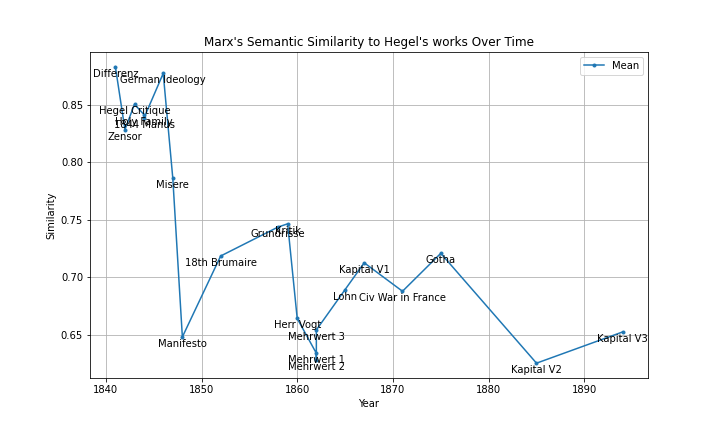
\includegraphics[width=\textwidth]{Emb0_Hegel_de_ts.png}
    \caption{Marx's similarity to Hegel, over time}
    \label{fig:hegelsims}
\end{figure}

Interestingly, given that many scholars locate Marx's departure from Hegel in his critical engagement with the latter's \textit{Philosophie des Rechts} in 1843, in terms of semantic content Marx's engagement with Hegelian \textit{themes} actually increases fairly dramatically after this time. This makes sense, however, if we consider the period roughly from 1843-1846 as a period wherein Marx aimed to distance himself from the Young Hegelians precisely by attacking their Hegel-oriented doctrines in the \textit{Holy Family} as well as the \textit{German Ideology}, and then the period from 1847 onward as his transition into his final economist phase. In fact, from what I can tell, the opening pages of the 1847 \textit{Misère de la Philosophie} are the first in which Marx explicitly identifies himself as an economist:

\begin{quote}
M. Proudhon has the misfortune to be uniquely misunderstood in Europe. In France he has the right to be a bad economist, since he passes for a good German philosopher. In Germany, he has the right to be a bad philosopher, because he passes as a prominent French economist. Being ourselves both German and economist, we have wished to protest against this dual mistake.\footnote{In Marx's original French: ``M. Proudhon a le malheur d'être singulièrement meconnu en Europe. En France, il a le droit d'être mauvais économiste, parce qu'il passe pour être bon philosophe allemand. En Allemagne, il a le droit d'être mauvais philosophe, parce qu'il passe pour être économiste français des plus forts. Nous, en notre qualité d'Allemand et d'économiste a la fois, nous avons voulu protester contre cette double erreur'' (\oldmega{I}{6}{19}; \textit{Misère} will also appear in its original French in the not-yet-published \mega{I}{6}).} (\mecw{6}{109}, as quoted in \cite{tribe_economy_2015})
\end{quote}


% Right after the German results

\subsubsection{French Republicanism: Calibration Tests}

To again establish our expectations with respect to what the similarity scores are capturing, we first show the similarity results for the set of Proudhon's texts included in our corpus.

%well-established relationships of direct influence:
%\begin{itemize}
%    \item[(a)] Saint-Simon vs. the ``Saint-Simonians''
%    \item[(b)] Babeuf vs. the ``Babeuvists'', and most importantly
%    \item[(c)] Proudhon vs. the ``Proudhonists''.
%\end{itemize}

These pairwise similarity scores between Proudhon's works are given in Table \ref{tab:proudhonself}.

\begin{table}[ht!]
\centering
\caption{Self-similarity between Proudhon's works, using the embedding-based measure}
\label{tab:proudhonself}
\begin{tabular}{lrrrr}
\toprule
{} &  Eigentum &  Nothwendigkeit &  Bekenntnisse &  Solution \\
\midrule
Eigentum       &    1.0000 &              -- &            -- &        -- \\
Nothwendigkeit &    0.9586 &          1.0000 &            -- &        -- \\
Bekenntnisse   &    0.9120 &          0.9316 &        1.0000 &        -- \\
Solution       &    0.9478 &          0.9529 &        0.8992 &    1.0000 \\
\bottomrule
\end{tabular}
\end{table}




\subsubsection{French Republicanism: Results}

Similarities between Marx's works and those of Proudhon are given in Figure \ref{fig:proudhonsims}, with the corresponding figures given in Table \ref{tab:proudhonsims}.

\begin{figure}
    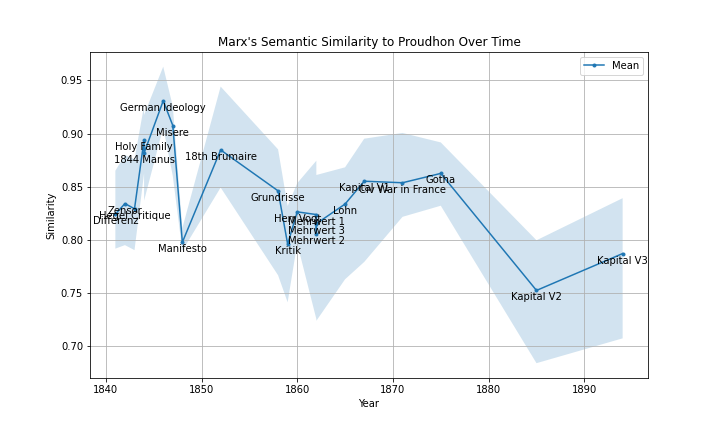
\includegraphics[width=\textwidth]{Emb1_Proudhon_de_ts.png}
    \caption{Marx's similarity to Proudhon, over time}
    \label{fig:proudhonsims}
\end{figure}

\begin{table}
\centering
\caption{Similarities between Marx's and Proudhon, over time}
\label{tab:proudhonsims}
\begin{tabular}{lrrrrr}
\toprule
{} &  Eigentum (1840) &  Nothwendigkeit (1847) &  Bekenntnisse (1848) &  Solution (1849) &   Mean \\
\midrule
Differenz (1841)         &           0.8072 &                 0.8651 &               0.8326 &           0.7919 & 0.8242 \\
Zensor (1842)            &           0.8231 &                 0.8389 &               0.8798 &           0.7952 & 0.8343 \\
Hegel Critique (1843)    &           0.8346 &                 0.8164 &               0.8759 &           0.7905 & 0.8294 \\
Holy Family (1844)       &           0.8733 &                 0.9263 &               0.9149 &           0.8627 & 0.8943 \\
1844 Manus (1844)        &           0.9176 &                 0.8992 &               0.8369 &           0.8733 & 0.8817 \\
German Ideology (1846)   &           0.9270 &                 0.9629 &               0.9277 &           0.9058 & 0.9308 \\
Misere (1847)            &           0.9188 &                 0.9257 &               0.8603 &           0.9257 & 0.9076 \\
Manifesto (1848)         &           0.7920 &                 0.8113 &               0.7899 &           0.7985 & 0.7979 \\
18th Brumaire (1852)     &           0.8493 &                 0.8711 &               0.9442 &           0.8740 & 0.8847 \\
Grundrisse (1858)        &           0.8749 &                 0.8579 &               0.7669 &           0.8852 & 0.8462 \\
Kritik (1859)            &           0.7980 &                 0.8132 &               0.7415 &           0.8320 & 0.7962 \\
Herr Vogt (1860)         &           0.7969 &                 0.8534 &               0.8274 &           0.8282 & 0.8265 \\
Mehrwert 1 (1862)        &           0.8746 &                 0.8370 &               0.7257 &           0.8585 & 0.8239 \\
Mehrwert 2 (1862)        &           0.8527 &                 0.8148 &               0.7152 &           0.8416 & 0.8061 \\
Mehrwert 3 (1862)        &           0.8611 &                 0.8243 &               0.7241 &           0.8520 & 0.8154 \\
Lohn (1865)              &           0.8683 &                 0.8456 &               0.7631 &           0.8581 & 0.8338 \\
Kapital V1 (1867)        &           0.8716 &                 0.8748 &               0.7794 &           0.8952 & 0.8553 \\
Civ War in France (1871) &           0.8218 &                 0.8537 &               0.9006 &           0.8392 & 0.8538 \\
Gotha (1875)             &           0.8917 &                 0.8645 &               0.8323 &           0.8619 & 0.8626 \\
Kapital V2 (1885)        &           0.7712 &                 0.7554 &               0.6843 &           0.7998 & 0.7526 \\
Kapital V3 (1894)        &           0.8119 &                 0.7903 &               0.7076 &           0.8393 & 0.7873 \\
\bottomrule
\end{tabular}
\end{table}



\subsubsection{British Political Economy: Calibration Tests}

As we did for German philosophy and French republican socialism, here we first examine the range of similarity measures our methods produce for a pair of books with an ``established'' relationship of influence: Adam Smith's \textit{Wealth of Nations} (1776) and David Ricardo's \textit{On the Principles of Political Economy and Taxation} (1817), given that the latter is in large part written as a response to Smith's groundbreaking 1776 work\footnote{Unlike in the previous two sections, here we opt not to compare Smith's \textit{Wealth of Nations} with e.g. his own earlier \textit{Theory of Moral Sentiments}, on the grounds that our aim is not to capture ``Smith-ness'' writ large, but rather ``political-economy-ness'' in the tradition established by \textit{Wealth of Nations}, rather than the less influential and more political-philosophy-oriented \textit{Theory of Moral Sentiments}. In Appendix \ref{app:robustness}, for transparency, we provide a version of Table \ref{tab:peself} which incorporates the \textit{Theory of Moral Sentiments} as well.}.

%set of ``established'' relationships of influence:
%\begin{itemize}
%    \item[(a)] Adam Ferguson vs. Adam Smith
%    \item[(b)] Adam Smith vs. David Ricardo, and
%    \item[(c)] John Stuart Mill's \textit{Principles} vs. David Ricardo's \textit{Political Economy}, of which the former work was explicitly written by Mill with the goal of ``formalizing'' the insights and contributions of the latter work.
%\end{itemize}

The results of these calibration tests are given in Table \ref{tab:peself}.

\begin{table}[ht!]
\centering
\caption{Self-similarity between Works of Political Economy, using the embedding-based measure}
\label{tab:peself}
\begin{tabular}{lrr}
\toprule
{} &  Wealth of Nations (2014) &  Grundgesetze (1877) \\
\midrule
Wealth of Nations (2014) &                    1.0000 &                   -- \\
Grundgesetze (1877)      &                    0.9400 &               1.0000 \\
\bottomrule
\end{tabular}
\end{table}



\subsubsection{British Political Economy: Results}

As can be seen in Figure \ref{fig:pesims} and Table \ref{tab:pesims}, Marx's ``Smith-ness'' increases significantly -- by over 10\% -- from his 1841 dissertation to his 1844 Manuscripts, then increases significantly but less rapidly in \textit{Poverty of Philosophy} and reaches a peak in 1858-1867 with the \grundrisse{}, the \kritik{}, the three volumes of \mehrwert{}, and \kapital{1}, with the notable exception of the extremely non-political-economic \textit{Herr Vogt}.

\begin{table}
\centering
\caption{Similarities between Marx's works and Works of Political Economy, over time}
\label{tab:pesims}
\begin{tabular}{lrrr}
\toprule
{} &  Grundgesetze (1838) &  Wealth of Nations (2014) &   Mean \\
\midrule
Differenz (1841)         &               0.7565 &                    0.7395 & 0.7480 \\
Zensor (1842)            &               0.7161 &                    0.7262 & 0.7211 \\
Hegel Critique (1843)    &               0.7289 &                    0.7224 & 0.7257 \\
Holy Family (1844)       &               0.7923 &                    0.7923 & 0.7923 \\
1844 Manus (1844)        &               0.8625 &                    0.8206 & 0.8416 \\
German Ideology (1846)   &               0.8606 &                    0.8441 & 0.8524 \\
Misere (1847)            &               0.9290 &                    0.9067 & 0.9178 \\
Manifesto (1848)         &               0.7718 &                    0.7709 & 0.7714 \\
18th Brumaire (1852)     &               0.7968 &                    0.7976 & 0.7972 \\
Grundrisse (1858)        &               0.9315 &                    0.8853 & 0.9084 \\
Kritik (1859)            &               0.8866 &                    0.8942 & 0.8904 \\
Herr Vogt (1860)         &               0.7584 &                    0.7286 & 0.7435 \\
Mehrwert 1 (1862)        &               0.9070 &                    0.8169 & 0.8620 \\
Mehrwert 2 (1862)        &               0.9174 &                    0.8133 & 0.8654 \\
Mehrwert 3 (1862)        &               0.9113 &                    0.8265 & 0.8689 \\
Lohn (1865)              &               0.9260 &                    0.8683 & 0.8971 \\
Kapital V1 (1867)        &               0.9314 &                    0.8985 & 0.9150 \\
Civ War in France (1871) &               0.7766 &                    0.7935 & 0.7850 \\
Gotha (1875)             &               0.8359 &                    0.7897 & 0.8128 \\
Kapital V2 (1885)        &               0.8654 &                    0.8077 & 0.8365 \\
Kapital V3 (1894)        &               0.9169 &                    0.8741 & 0.8955 \\
\bottomrule
\end{tabular}
\end{table}


\begin{figure}
    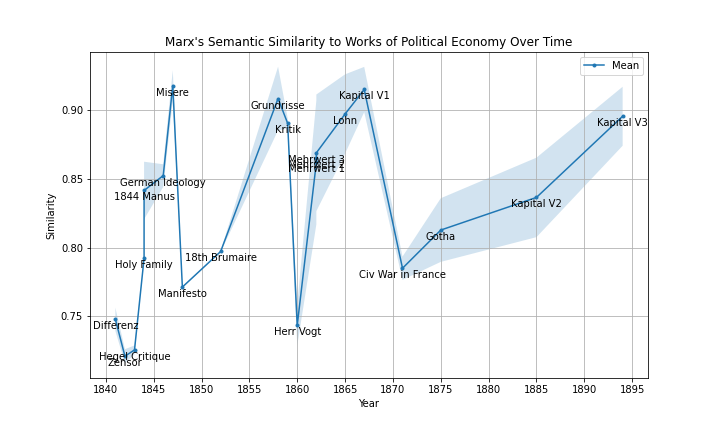
\includegraphics[width=\textwidth]{Emb2_PolEcon_de_ts.png}
    \caption{Marx's similarity to works of Political Economy, over time}
    \label{fig:pesims}
\end{figure}


%%%%% PART II %%%%%

\section{Part II: Marx's Influence}

\subsection{Introduction}

Perhaps the single key driver of the development of Marx's thought over the course of his life was his almost obsessive impulse to engage in polemics with those he viewed as obstacles to (in his early years) or rivals to (in later years) his assumption of the throne as the intellectual leader of the 19th century European socialist movement. We have already encountered this tendency in previous sections, when discussing the development of his thought with respect to the ``stationary targets'' of his criticism---namely, the already-established big names in political economy, early socialism, and philosophy such as Adam Smith, David Ricardo, Henri de Saint-Simon, and Hegel. In this section we turn to Marx's ``forward-facing'' polemics against his various interlocutors, his critique of the ``moving targets'' vying with him for intellectual influence over the quickly-growing European socialist movements of the era.

Central to this section is the move from \textit{influences} to \textit{interlocutors}. While Marx could isolate himself in his studies of the former for as long as he needed to develop cogent critiques, the European socialist movement moved at its own pace, requiring his critiques of the latter to be not only cogent but \textit{timely} as well. Engels, for example, urged Marx in 1845 to complete and publish his already-in-progress politial-economic tract as soon as possible, emphasizing that ``people's minds are ripe and we must strike while the iron is hot''\footnote{\mew{27}, p. 16.}. The urgency heightened even more when, in the ensuing year, the prominent French socialist Pierre-Joseph Proudhon published his own such tract titled \textit{Système des contradictions économiques}. As Keith Tribe puts it in his insightful analysis of Marx's subsequent polemics with Proudhon, ``the publication of Proudhon’s \textit{Système} galvanised [Marx] into writing a shorter work so that he might stake his claim to being Western Europe's foremost `radical political economist'. [Marx's 1847] \textit{Misère de la philosophie} is primarily a bid for market leadership, and it certainly reads that way.'' (\cite{tribe_economy_2015}, p. 224) 

Similarly, after having spent a decade in exile in London desperately working to maintain his relevance within the growing socialist movement of his home country, the 1859 publication of an attack on him in a German newspaper persuaded him to drop his political-economic studies for nearly two years in order to craft a response which would quell the ``foggy gossip of the [1848] refugees''\footnote{\mew{30}, p. 17.}. The attack, penned by a minor figure from the 1848 Frankfurt Assembly named Karl Vogt, cajoled Marx into working full-time to collect evidence against Vogt, culminating in a 208-page work, \textit{Herr Vogt}, for which he was never able to find a German publisher. Thus, in the remainder of the section, we take seriously the centrality of these ``wars of ideas'' in the development of Marx's thought by turning to an analysis of his illocutionary moves---what he was \textit{doing} with these polemical interventions, and how exactly he positioned himself within ideological spaces, in a way which eventually succeeded in crowding out all other contenders.

While some polemical episodes are not considered herein---for example, his 1847 polemic against Karl Heinzen after the latter's attack on Engels in the \textit{Deutsche-Brusseler Zeitung}\footnote{Culminating in the article ``Moralising Criticism and Critical Morality. A Contribution to German Cultural History. Contra Karl Heinzen'', published in the same newspaper in October and November of that year. \mecw{6}, p. 312.}, or his 1865 debate with his fellow International Working Men's Association (IWMA) General Council member John Weston\footnote{Culminating in an 1865 address to the IWMA in which Marx introduced his mature political-economic views (published long-form in the first volume of \textit{Das Kapital} two years later), which was published posthumously in the form of a pamphlet entitled \textit{Value, Price, and Profit}. }---we focus on four such episodes that were particularly impactful, we argue, with respect to the development of Marx's thought. We begin with his first major ``public break'' (his break with the liberalism of his father and schoolmasters in Trier, via his turn to Hegel in the late 1830s, only being known to us by way of his private letter to his father cited previously), his polemics against the pure philosophizing of the Young Hegelians between 1843 and 1845, culminating in his justly famous ``Theses on Feuerbach'' which asserted his commitment to a philosophy of \textit{praxis} -- a commitment to \textit{engaged} philosophy which aimed not only to understand society but also to change it.

Next we move to the period from 1845 to 1849, characterized by the buildup to and eventual defeat of the 1848 revolutions which swept across Europe. We focus especially on his critique of ``state socialists'' like Louis Blanc here, since this became a central focal point around which socialist polemics swirled after Blanc's appointment to the revolutionary provisional government in 1848, where he was expected to begin implementing his scheme for ``national workshops'' as outlined in his tract \textit{Organization of Labor} (1840)\footnote{In reality, Blanc was almost completely hamstrung in these efforts from the start, and almost surely doomed to failure. While public perception, shrewdly encouraged by his opponents, was that he had been tasked with implementing the workshops, in fact he had only been appointed to head the ``Luxembourg Commission'' where he battled with his cynical rival representatives just to complete a report on the feasibility of his schemes, thus keeping him preoccupied while forces of reaction and monarchical restoration worked to defeat the gains of the revolution outside of these meetings. See, e.g., \cite{agulhon_republican_1983}.}

\subsection{Marx's Interlocutors}

\subsubsection{The Young Hegelians, 1843--1845: Bruno Bauer and Max Stirner\label{sec:hegelians}}

Although he had planned to write critiques of particular contemporary authors like Hermes or Rosenkranz as early as 1839, it was his critique of Hegel's Philosophy of right in 1843 that scholars typically point to as marking the beginning of Marx's period of ``committed'' polemics against the Young Hegelian milieu which he had initially identified himself as part of. After the Critique of Hegel's Philosophy of Right, his first true engagement with a Hegelian ``interlocutor'' (as opposed to Hegel himself, who had been dead for 12 years when Marx wrote the Critique of his Philosophy of Right) came in the form of his writing ``On the Jewish Question''. The themes of this work were further expanded upon, and the scope of his polemics expanded to include Max Stirner and Ludwig Feuerbach, in his first joint work with Engels in 1844, \textit{The Holy Family}. Marx considered this work to be his ``final break'' with the Young Hegelians, with the exception of Feuerbach -- his final break with the latter would not come until his second joint work with Engels, the \textit{German Ideology}, written in 1846 but never published in Marx's or Engels' lifetime (in fact, not published until the 1930s).

``the sovereign
derision that we accord to the Allsemeine Literatur-Zeituns is in stark
contrast to the considerable number of pages that we devote to its
criticism'.'' Engels to Marx

\subsubsection{``State Socialism'' I, 1845--1849: Louis Blanc\label{sec:blanc}}

Although a number of works have explored Marx's views on the State in detail (e.g., \cite{hunt_political_1974} and \cite{hunt_political_1984}; \cite{draper_karl_1977-1}; and \cite{leipold_radical_2020}, Ch. 7), these investigations typically focus on Marx's work after the rise and fall of the Paris Commune in 1871, especially his 1875 \textit{Critique of the Gotha Programme}. In this section, however, we hope to draw more attention to Marx's (admittedly more opaque and imprecise) work from an earlier era, namely, the years leading up to the 1848 revolutions. In his writings from this period one can already infer the main characteristics of Marx's burgeoning socialist conception of the state, especially in his criticisms of European ``state socialists'' like Louis Blanc who envisioned a non-revolutionary path to socialism set into motion by the introduction of universal suffrage and constitutional constraints on power.

\subsubsection{Anarchism I, 1846--1849: Pierre-Joseph Proudhon\label{sec:proudhon}}

Pierre-Joseph Proudhon's thought, as our quantitative analysis will corroborate, 
%was the result of 
was an eclectic and self-taught mixture of his 1830s engagement with theology and philology in the 1830s with his subsequent engagement---predating Marx's own by a few years---with British political economy and Hegelian philosophy. In fact, although details on their engagement are scarce\footnote{Scarce despite numerous research endeavors, typically in the same anarchists-versus-Marxists vein as the studies on Marx and Bakunin described in more detail in Section \ref{sec:bakunin} below).}, some researchers accept Marx's post-falling-out contention that he taught Proudhon everything he knew about Hegel.

In fact, although most works on the early development of Marx's thought contend that Marx's transition from Young Hegelianism to British political economy was driven by Engels' 1843 engagement with the latter, published in his ``Umrisse'', a good case could be made for the hypothesis that Proudhon played a not-insignificant role. As a comparison of their reading notebooks (Table \ref{tab:reading}) attests, Proudhon had already read many of the texts noted as central to this Engels-to-Marx transmission three or four years before Marx began studying them.

\begin{table}[ht!]
    %\begin{minipage}{\linewidth}
    \centering
    \begin{threeparttable}
    \begin{tabularx}{\linewidth}{Xcc}\toprule
        \textbf{Text} & \textbf{Proudhon} & \textbf{Marx} \\\midrule
        
        Adam Smith, \textit{Wealth of Nations} (1776) & Oct 1841 & Mar--Aug 1844 \\
        % cahier XXIII (oct 1841) (6-12), p. 1090
        % again, cahier premier de 1844, jun-july (ed. Blanqui) (18-45), p. 1092
        % First mentioned in comments on james mill
        
        David Ricardo, \textit{Principles} (1817) & Oct 1841 & 1844 \\\midrule
        % cahier XXIII (oct 1841) (42-48), p. 1090
        % First referenced in econ+phil manus of 1844
        
        Charles Comte, \textit{Traité de la propriété} (1834) & 1839 & --- \\
        % cahier I in-4, p. 1081
        % also, cahier X (1839) (p. 15-20), p. 1086
        
        F. X. J. Droz, \textit{Propriété} (1832) & 1839 & 1846 \\
        % cahier I in-4, p. 1081
        
        A. Destutt de Tracy, \textit{Économie politique} (1823) & 1839 & Oct 1843-1845 \\
        % cahier II in-4 (p. 17-29), p. 1081
        
        Adolphe Blanqui, \textit{Hist. de l'econ. pol.} (1837) & 1839 & 1845 \\
        % cahier VI in-4 (p. 15), p. 1083
        
        Dugald Stewart, \textit{Esquisses de phil. morale} (1793) & 1839 & 1858--1862 \\
        % cahier III (1839) (p. 19-22), p. 1084
        
        J. B. Say, \textit{Cours complet de Écon. pol.} (1828) & 1839 & Oct 1843--1845 \\
        % cahier VII (1839) (p. 29-48), p. 1086
        
        A. A. Cournot, \textit{Principes mathém. d'Écon. pol.} (1838) & 1839 & --- \\
        % cahier X (1839) (p. 27-28), p. 1086
        
        P. Rossi, \textit{Cours d'Écon. pol.} (1836) & Jan 1840 & 1845 \\
        %  cahier XI (6 jan 1840) (3-4), p. 1087
        % again cahier XXIII (oct 1841) (book 1) (12-42), p. 1090
        % again cahier XXIV (nov 1841) (book 2) (21-38), p. 1090
        
        G. Garnier, \textit{Da la propriété} (1792) & Nov 1840 & ---
        % cahier XV (nov 1840) (35-36), p. 1088
        
        % Marx did, in 1863, read Garnier's 1796 S. 132-145: Germain Garnier , Abrégé élémentaire des principes de l'économie politique , 1796. IISH B103
        \\
        
        %Buchez & 1840 & & \\
        
        %Bentham & 1841 & & \\
        
        %C. Fourier, \textit{Traité d'association} (1822) & Sep 1841 & --- & --- \\
        % Engels read Charles Fourier , Nouveau Monde Industriel et Sociétaire , ab ± 1877?, franz. ½ S
        % S. 8-10: Ch. Fourier , Theorie des 4. Mouvements , 1846.
        
        %Considérant, \textit{Politique générale} & Sep 1841 & & \\
        
        %Cabet, \textit{Icarie} & Sep 1841 & & --- \\
        
        A. Ciezkowski, \textit{Du crédit et de la circulation} (1839) & Oct 1841 & --- \\
        % cahier XXII (oct 1841) (3-34), p. 1090
        
        %P. Leroux, \textit{l'Humanité} (1840) & Jan 1842 & & \\
        
        %Buret, \textit{De la misère} (1840) & 1844 & & \\
        
        %G. Garnier, preface to Smith & Jul 1844 & & \\
        
        %M. Chevalier, Cours d'Econ. pol.
        % Le premier de 1844, (1841-1842) (15-18), p. 1091
        
        %Sismondi, \textit{Études sur l'Écon. pol.} (1837-38) & Jul 1844 & & 1845\tnote{z} \\
        % le second cahier, jul 1844, etudes (book 2) (1838) (19-38), p. 1092
        % B30 S. 7--19 (Brussels)
        
        %W. Godwin, \textit{Recherches} & Jul 1844 & & \\
        
        %L. Blanc, \textit{Histoire de dix ans} & Jan-May 1844 & & ---\tnote{z} \\
        \bottomrule
    \end{tabularx}
    \end{threeparttable}
    %\footnotetext{\cite{rubel_marx_1975} claims, however, that Marx ``presumably read'' Ciezkowski's \textit{Historiosophie}, however.}
    %\end{minipage}
    \caption{A comparison of the dates of first reading for key political-economic texts, as recorded in Proudhon's and Marx's respective reading notebooks. On Proudhon's reading notebooks, see Appendix \ref{app:proudhoncarnets}. On Marx's, see Appendix \ref{app:marxreading}. Entries after Smith and Ricardo are listed in the order in which they appear in \cite{haubtmann_pierre_1982}. Sources for each date of reading are given in Appendix \ref{app:tablefn}.}
    \label{tab:reading}
\end{table}

\subsubsection{Challengers to the Throne I, 1859--1860: Karl Vogt\label{sec:vogt}}

As chronicled by several of his biographers, Marx's political-economic writing incurred several major interruptions in the form of protracted polemics against other socialists whom Marx viewed as potential opponents (or perhaps saboteurs) for hegemony over European socialist discourse. In 1859 and 1860 for example, after the publication of his \textit{Zur Kritik}, Marx abruptly ceased working on his ``Economics'' and began a polemic with Karl Vogt, a minor figure from the 1848 Frankfurt Parliament who had slandered him in a German newspaper. The extent to which his need to strike back suddenly superceded all other concerns is aptly described by David McLellan in his biography of Marx:
\begin{quote}
This quarrel, which occupied Marx for eighteen months, is a striking example both of Marx's ability to expend tremendous labour on essentially trivial matters and also of his talent for vituperation. (\cite{mclellan_karl_1973}, p. 311)
\end{quote}
Even Engels himself, normally supportive of Marx in all his endeavors, diplomatically begged the latter not to allow the ``Vogt affair'' to interrupt his political-economic studies:
\begin{quote}
The prompt appearance of your second installment\footnote{Referring to the ``sequel'' to Marx's 1859 \textit{Contribution to the Critique of Political Economy} (\textit{Zur Kritik der Politischen Ökonomie}), i.e., to the work that would eventually coalesce into the three volumes of \textit{Das Kapital}.} is obviously of paramount importance in this connection and I hope that you won't let the Vogt affair stop you from getting on with it. [...] I am very well aware of all the other interruptions that crop up, but I also know that the
delay is due mainly to your own scruples.
\end{quote}
Marx did not heed Engels' plea, however, and pressed onwards with his 18 months of work on what was to become the 208-page \textit{Herr Vogt}. Characteristically, however, Marx was never able to find a German publisher, thus defeating the entire purpose of the work in the first place.

% 473 After the publication, in June 1859, of the first instalment of A Contribution to the Critique of Political Economy (see present edition, Vol. 30), Marx intended, as previously agreed with the Berlin publisher Duncker, to prepare for the press and publish as the second instalment the 'Chapter on Capital', which constitutes the bulk of his main economic manuscript of 1857-58; and then publish the remaining parts of his economic work (see Notes 250 and 355).

% As he proceeded with his plan, however, he realised that he would have to do more research to formulate the basic propositions of his economic theory. But his journalistic activity and other party obligations, above all the need to refute publicly Vogt's slanderous allegations against proletarian revolutionaries, temporarily diverted him from his economic studies. It was not until 1861 that he resumed them in earnest. Later Marx decided to publish his researches not as the second and further instalments of A Contribution to the Critique of Political Economy but as a large independent work.—489, 498, 502, 508, 511, 522, 523, 542, 574

\subsubsection{``State Socialism'' II, 1864--1883: Ferdinand Lassalle\label{sec:lassalle}}

Ferdinand Lassalle, a German socialist intellectual and agitator\footnote{The rendering of his surname as ``Lassalle'' is actually a Gallicization of his family name, Lassal, a spelling he promulgated early on to deflect attention away from his Silesian origins, as part of his goal to establish himself as a radical intellectual in Paris starting in the mid-1840s.} played a variety of seemingly-incongruous roles in the development of Marx's post-1848 social and economic thought. A study of \textit{MEGA}², for example, would give an impression of Lassalle as someone with whom Marx tried to remain on good terms via his direct correspondence, despite harboring an intense disdain towards him (which comes out in his descriptions of Lassalle in letters to Engels over the same time period), a balancing act which was ``resolved'' by Lassalle's early death after an 1864 duel. If one takes into account late-19th-century developments in European socialism immediately before and after the 1875 establishment of the German SPD, however, it emerges that in fact Lassalle's immense posthumous influence outlived even Marx himself. It wasn't until Engels' work moulding the ideology of the SPD for 12 years following Marx's death that Lassalleanism was ``defeated'' as a viable competitor to Marxism among European socialists.


\subsubsection{Anarchism II, 1872--1883: Mikhail Bakunin\label{sec:bakunin}}

Mikhail Bakunin, hailed by some as the father of modern anarchism, is typically cast in the role of Marx's main rival in the First International between 1868 (the year Bakunin joined) to 1872 (when Bakunin and his followers were expelled by Marx), in socialist and anarchist histories alike (see, e.g., \cite{eckhardt_first_2016}). Interestingly, however, Marx and Bakunin crossed paths fairly regularly, in substantial ways, from 1840 onwards. To name just one rarely-mentioned instance, Bakunin produced the first Russian translation of the \textit{Communist Manifesto}, which was published in the periodical \textit{Kolokol} in London in 1860\footnote{See \cite{guillaume_internationale_1905}, p. 283, cited in \cite{favilli_history_1996}. Bakunin had a number of path-crossings with Engels over the years, as well. They were both in attendance, for example, at F. W. J. Schelling's infamous 1841 lectures at the University of Berlin (\cite{hunt_marxs_2010}, 44--46).}. Starting the narrative of the Marx-Bakunin relationship in 1864, therefore, ignores a great number of interactions which impacted the development of Marx's thought.

Bakunin moved from Moscow to Berlin in 1840 to enroll at the University of Berlin---the same university where Marx had been studying since 1836---and quickly became a prominent figure in the Young Hegelian movement alongside Marx, Bruno and Edgar Bauer, and Arnold Ruge. Bakunin and Marx both, in fact, contributed articles to Ruge's \textit{Deutsche Jahrbücher fur Wissenschaft and Kunst} in 1842, though Marx's contribution (ironically, a commentary on Prussian censorship restrictions) was censored by the Prussian government and only published a year later in Switzerland. After the Prussian government banned this publication outright in 1843, Marx and Ruge moved to Paris to co-found the \textit{Deutsche-Franzosische Jahrbücher}, with Bakunin joining them in the city that same year. After finally meeting in person in 1844, Marx and Bakunin corresponded in a mostly-cordial fashion for decades, up until the 1872 split of the First International. Even as late as 1871, for example, Bakunin accepted a commission to produce the first Russian translation of Volume 1 of \textit{Das Kapital}, a work which he deeply admired, having earlier commented that ``no other work that I know of puts together such a profound, enlightening, scientific, decisive analysis'' of the capitalist economy.

The 1872 split and the four years leading up to it---an episode of Marx's life which Alvin W. Gouldner calls ``the culminating conflict of [Marx's] political life'' (\cite{gouldner_marxs_1982})---have been exhaustively documented in two parallel literatures, which present two starkly contrasting narratives. The first narrative, promulgated most heavily in the Soviet Union, sees Marx effortlessly fusing theoretical insight with organizational prowess, keeping the International sharply focused on its proletarian revolutionary aims despite the best efforts of the saboteur Bakunin\footnote{See \cite{nicolaievsky_karl_1936}, pp. 280--297, for a fairly inocuous example.}. The second narrative, promulgated by both Western anti-Soviet historians and anarchists in nearly identical forms, sees Marx ruthlessly stamping out any and all anti-authoritarian voices in the International, with Bakunin finally giving up on his noble but quixotic efforts in 1872 to found the aptly-named Anti-Authoritarian International\footnote{A stark example of this contrasting narrative can be found in \cite{eckhardt_first_2016}.}.
%(from which a direct line can be traced to the present-day IWA-AIT\footnote{Short for the International Workers' Association---Asociación Internacional de los Trabajadores, whose Spanish section constitutes the major Spanish trade union CNT (Confederación Nacional del Trabajo).})

For the purposes of this work, however, it suffices to say that Marx viewed Bakunin as a key rival for leadership of the European socialist movement. Public perception and commentary on this movement, especially in the years leading up to the split, often compared the two, adding fuel to Marx's competitive fire. The Italian socialist newspaper \textit{La Plebe}, for example, characteristically referred to Marx as ``Germany's Bakunin'' in a major article of January 1872\footnote{``Lettere da Berlino'', \textit{La Plebe}, Jan. 5, 1872, cited in \cite{favilli_history_1996}, p. 32. See \textit{ibid.} pp. 20--46 for an in-depth discussion of the Bakunin-Marx rivalry and its relation to 19th-century Italian socialist thought.}. Hence, as is the case with nearly all of his works, Marx's discursive interventions throughout the era of the First International were driven primarily by polemical concerns. 

Just as it is inappropriate to begin the Marx-Bakunin narrative in 1868, it is also inappropriate to end it with the 1872 split. Two years after the split, in April of 1874, Marx began reading Bakunin's \textit{Staatlichkeit und Anarchie} (\textit{Statism and Anarchy}). By the time he finished in January of 1875, he had copied 224 separate extracts into his notebook in Russian, some spanning several pages. He provided extensive commentary on 39 of these, breaking out of the extracts and writing paragraph-length or even page-length responses, in addition to the shorter inline comments he made on nearly all of them (ranging from single exclamation points to parenthetical definitions, translations, and quips)\footnote{Our calculations, based on \mew{18}, pp. 597--642.}.



\subsubsection{Challengers to the Throne II, 1883--1884: Eugen Dühring\label{sec:duhring}}

When in the post-\textit{Kapital V1} years another contender for Marx's historiographic crown emerged, Eugen Dühring, Engels (having learned from the Karl Vogt episode) consciously opted to take the lead and conduct the polemics himself so Marx could carry on with his work on \textit{Kapital}. Although Marx did end up contributing in a non-trivial way to the resulting book \textit{Herr Eugen Dühring's Revolution in Science} (typically shortened as \textit{Anti-Dühring}), it was published under Engels' name in 1884, a year after Marx's death.

Unlike in the case of Vogt, however, Dühring was a worthy opponent, a major intellectual figure in Germany who wielded great influence and thus directly challenged the recently-acquired gains in Marx's prominence and notoriety after the rise and fall of the Paris Commune. Dühring's published works would have an immediate and substantial impact on German political-philosophical discourse---albeit an impact fairly distant from the epicenters of socialist discourse---with Friedrich Nietzsche being only one of many prominent post-Hegelian thinkers who were profoundly influenced by Dühring\footnote{Nietzsche's reading included nearly all of Dühring's published works, some of which he read on multiple occasions---see the supplemental dataset on Nietzsche's known and conjectured reading described and linked in Appendix \ref{app:suppdata}. For a summary of the main trends in post-Hegelian German philosophy, see \cite{beiser_after_2014}, pp. 172--184 (``Dühring on the Value of Life''), where Dühring's ``important place in the history of nineteenth-century philosophy'' includes his role as ``the founder of  German positivism, the grandfather of Schlick, Carnap, Neurath, and Reichenbach.'' (p. 174)}.


\subsection{Methods}

\subsubsection{Author-Specific Embedding Spaces}

Although the embedding methods described in Section \ref{sec:methods} allowed us to construct a \textit{single} ideological space within which we were able to compare Marx's writings with those of his posited influences, in this section we need a more advanced technique which will allow us to trace the differential usage of various terms both over time and across authors (or groups of authors). Thus, for the explorations in this section we utilize a newer method introduced in
\cite{welch_exploring_2020}, %\cite{personalized_2018},
that of ``personalized'' word embeddings. While still estimating an overall ideological space based on the entire corpus (labeled \texttt{MAIN} in the resulting dataset), this approach also allows us to label each text with an author, for whom a separate set of embedding vectors is estimated.

Importantly, this method does not generate a separate embedding \textit{space} for every author, since one author's vectors need to be comparable with any other author's vectors\footnote{i.e., for authors $A$, $B$, and $C$, the distance $d(\vv{w_A}, \vv{w_B})$ between $A$'s vector for some word $w$ and $B$'s vector for $w$ must be on the same scale as the distance $d(\vv{w_A}, \vv{w_C})$ between $A$'s vector for $w$ and $C$'s vector for $w$, as well as the distance $d(\vv{w_B}, \vv{w_C})$ between $B$'s vector for $w$ and $C$'s vector for $w$.}. Instead, each author's specific vector $\vv{w_i}$ for a given term $w$ is estimated as some offset relative to the vector for $w$ in the \texttt{MAIN} vector space, $\vv{w_\texttt{MAIN}}$. Given a vector $\vv{w_{PE}}$ representing the centroid of political-economic discourse within the broader ideological vector space (estimated via a procedure we detail in the next section), for example, this allows us to instantly check whether an author $A$ tends to use a term $w$ in a more political-economic context than some other author $B$, by checking whether $d(\vv{w_A},\vv{w_{PE}}) < d(\vv{w_B},\vv{w_{PE}})$, or relative to the ``average'' usage of the term across the entire corpus, by checking whether $d(\vv{w_A},\vv{w_{PE}}) < d(\vv{w_\texttt{MAIN}},\vv{w_{PE}})$.

A problem arises, however, if we try to estimate an author-specific vector for an author with very few texts in the corpus, akin to e.g. the problem of statistical power in regression estimation. To address this issue, we instead group individual authors into ``meta-authors'' based on the discursive community they are generally associated with in the historical literature. Thus, for example, the texts of Bruno and Edgar Bauer, Arnold Ruge, Max Stirner, etc., are combined into one Young Hegelian meta-author in order to estimate a vector $\vv{w_{YH}}$ representing the centroid of Young Hegelian discourse (as defined by this author-to-group mapping) within the broader ideological space of 19th-century German discourse. Importantly, however, this approach is \textit{not} used to generate the political-economic and Hegelian vectors which serve as our orthogonal basis vectors, for reasons we describe in the next section.


\subsubsection{Discursive Fields as Embedding Clusters}

As mentioned in the previous section, there are two special vectors $\vv{w_{PE}}$ and $\vv{w_H}$, representing the centroids of political-economic and Hegelian discourse respectively, which we do \textit{not} compute via author-specific embedding estimation. Instead, to minimize the dependence (in the statistical sense) between our two basis vectors and the vectors like $\vv{w_{Marx}}$ for which we want to observe movement over time, we compute these basis vectors as centroids of word clusters which are derived independently via the cTFIDF measure, which generates a ranking of all terms in the corpus on the basis of how ``unique'' they are to political-economic texts relative to Hegelian texts (and vice-versa, by taking the $N$ terms with lowest, rather than greatest, cTFIDF scores).


\subsection{Results: Marx and the Socialist Movement}

As can be seen in Figure \ref{fig:cambresult}, we indeed observe a time-lagged movement of the Socialist centroids for each decade in the same direction as Marx's, namely, in the direction moving away from the Hegelian centroid and towards the political-economic centroid, from 1840 onwards (interestingly, after a move \textit{towards} the Hegelian centroid between 1830 and 1840).

\begin{figure}[ht!]
    \centering
    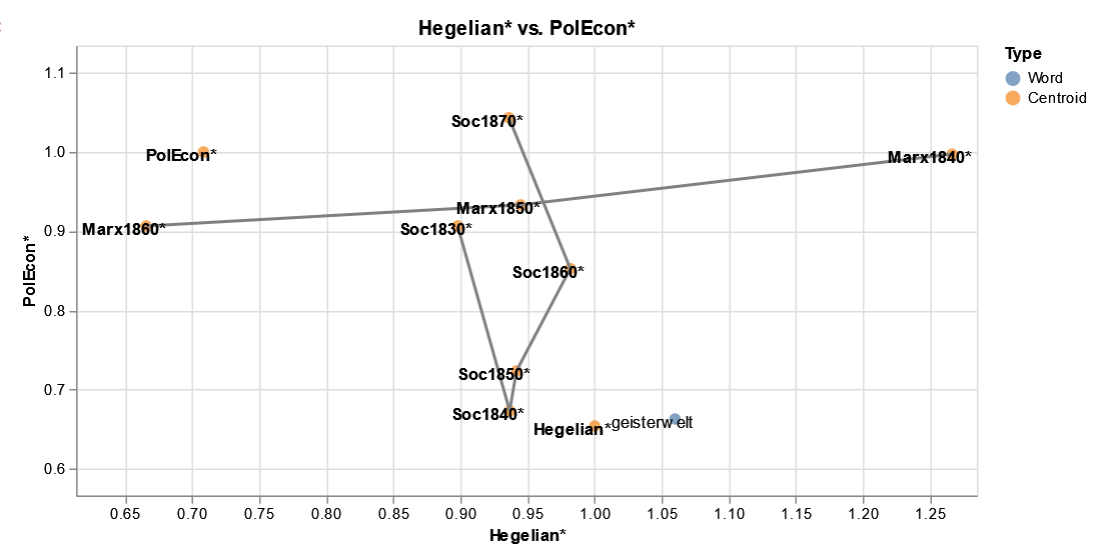
\includegraphics[width=\textwidth]{camb_result.png}
    \caption{The trajectories of Marx's decade-by-decade centroids and the decade-by-decade centroids of European socialist discourse, with respect to the static Hegelian (defining the x-axis) and Political-Economic (defining the y-axis) centroids.}
    \label{fig:cambresult}
\end{figure}

\begin{figure}[ht!]
\centering
\includesvg[width=\textwidth]{rolling_pe_sim.svg}
\caption{Rolling PE Similarity Scores for Marx's Collected Writings}
\end{figure}

\begin{figure}[ht!]
  \centering
  \includesvg[width=\textwidth]{pe_centroid.svg}
  \caption{A Principal Component Analysis (PCA) plot of the Political Economy centroid with the top $N = 25$ words most distinctive to this subcorpus.}
  \label{fig:pecentroid}
\end{figure}

\begin{figure}[ht!]
  \centering
  \includesvg[width=\textwidth]{heg_centroid.svg}
  \caption{A Principal Component Analysis (PCA) plot of the Hegelian centroid with the top $N = 25$ words most distinctive to this subcorpus.}
  \label{fig:hegcentroid}
\end{figure}

\begin{figure}[ht!]
  \centering
  \includesvg[width=\textwidth]{comb_centroid.svg}
  \caption{A plot of the two centroids used to define the ideological subspace (Political Economy and Hegelian), along with the top $N = 25$ words most distinctive to either subcorpus.}
  \label{fig:combcentroid}
\end{figure}


\subsection{Results: Marx vs. Particular Authors\label{sec:marxvauthors}}

Although tracking the literary output of Marx's interlocutors is generally a much more difficult task than tracking Marx's own\footnote{Ostensibly due to the fact that, unlike Marx, most 19th-century thinkers did not end up having a global superpower collecting and propagating their texts---on this topic, see our discussion of the Soviet ``weaponization'' of Marxism in \cite{jacobs_quantifying_2021}.}, a few collections of key rivals exist which enable us to ``break apart'' the Socialism vector into vectors for particular authors. With these individual-author vectors, we can evaluate which authors in particular had trajectories which drove the overall shift observed in the previous section.

Pierre-Joseph Proudhon's writings are of special interest with respect to the computational nature of this work, since not only do we have his collected writings but also newly-digitized scans of his notebooks, the \textit{Carnets}, containing (as in the case of Marx) not only drafts of his works at various stages but also the meticulous reading notes and extracts he kept over the course of his life. An overview of this dataset, used throughout our analysis in Section \ref{sec:marxvproudhon} below, is given in Section \ref{sec:proudhon} above, with more details provided in Appendix \ref{app:proudhoncarnets}\footnote{For an overview of the \textit{Carnets} in general, see the section entitled ``Notes et Annotations Diverses'' in the Appendix of \cite{haubtmann_pierre_1982}, pp. 1079--1098.}.

As for his main body of writings---those which were intended for public consumption---several large collections have been compiled, starting as early as 1850 when he was still actively publishing new works. This first 26-volume collection was completed in 1872, and scans of each volume are available through the Bibliotheque National de France's Gallica portal at \href{https://catalogue.bnf.fr/ark:/12148/cb31154797t}{https://catalogue.bnf.fr/ark:/12148/cb31154797t}.

A comparison of Marx's writings with those of Ferdinand Lassalle, somewhat in contrast to the case of Proudhon, lets us analyze Marx's speech acts as a self-consciously \textit{political} rather than economic actor. While (as argued in Section \ref{sec:proudhon} above) Marx explicitly aimed to distinguish himself as a ``better'' economist than Proudhon, it was Lassalle's political principles and their manifestations in e.g. the Gotha Programme of 1875 (and the Erfurt Programme of 1891, in Engels' posthumous efforts his behalf) that Marx explicitly worked to repudiate and replace with his own.

Due to his prominence in the eyes of Second International-era SPD intellectuals like Eduard Bernstein, new collections of Lassalle's writings were compiled and published quite frequently from 1865 (starting with J. P. Becker's collection published just one year after Lassalle's death) up until the Nazi regime's rise to power. Although some additional collected-works projects were carried out in the GDR from 1949 onwards, three collected-works projects from the SPD era remain basically the canonical reference texts for scholarship on Lassalle to this day. The most commonly-referenced collection, the \textit{Gesammelte Reden und Schriften} (GRS), was edited by Eduard Bernstein and published in 12 volumes from 1919 to 1920, while a second collection, the \textit{Nachgelassene Briefe und Schriften} (NBS), was edited by Gustav Meyer and published in 6 volumes between 1921 and 1925, augmenting the corpus of the earlier 12-volume project with (for example) posthumously-discovered letters and earlier drafts of major speeches found in his notebooks\footnote{Links to each volume are given in Appendix \ref{app:lassallecw}.}. A third collection, Eduard Bernstein's 1898 \textit{Reden und Schriften} (RS) in 3 volumes, is referenced less often but remains influential nonetheless due to its status as the canonical reference for Lassalle's writings from the year of its publication up until the 1920s (when, as the later volume's title suggests, Bernstein's 12-volume GRS supplanted the 3-volume RS)\footnote{It is important to note, however, that (for reasons which are not made entirely clear in Bernstein's introduction) there are some texts in the RS which were \textit{not} carried over into the GRS. For 6 of the 100 texts listed in Andréas' bibliography, therefore, we had to scrape the plaintext by OCRing scans of the original RS, which are of far lower quality than the available scans of the GRS and NBS. As explained in Appendix \ref{app:lassallebib}, however, these 6 texts can be identified and excluded from any analysis by filtering out texts whose \texttt{source} metadata variable is equal to \texttt{"RS"}.}.

More recently, researcher Bert Andréas' valuable bibliography \citep{andreas_ferdinand_1981} contains entries for all known writings of Lassalle, along with known translations and information on differences (e.g., inclusion, exclusion, and modification of the original text) between subsequent editions and printings.

The compilation of our Lassalle dataset, which pairs digital plaintext versions of all his known writings with metadata on each text (e.g., date of writing and/or publication, data on all known versions, on all known translations, etc.), was aided immensely by our digitization of Andréas' bibliography. The resulting diachronic corpus of Lassalle's writings is analyzed in Section \ref{sec:marxvlassalle} below and discussed in detail in Appendix \ref{app:lassallebib}.

Mikhail Bakunin's complete works in German have been published in 3 volumes in an edition titled \textit{Gesammelte Werke} edited by Max Nettlau, available for full viewing at \href{https://catalog.hathitrust.org/Record/012322886}{HathiTrust}.
%A 6-volume selection of works was also published.
In French, there also exists a 6-volume \textit{Oeuvres} available at the \href{https://archive.org/details/oeuvresbs01bakuuoft}{Internet Archive}\footnote{Volume by volume links to this French collection are as follows: \href{https://archive.org/details/oeuvresbs01bakuuoft}{Volume 1}, \href{https://archive.org/details/oeuvresbs02bakuuoft}{Volume 2}, \href{https://archive.org/details/oeuvresbs03bakuuoft}{Volume 3}, \href{https://archive.org/details/oeuvresbs04bakuuoft}{Volume 4}, \href{https://archive.org/details/oeuvresbs05bakuuoft}{Volume 5}, \href{https://archive.org/details/oeuvresbs06bakuuoft}{Volume 6}.}.

However, as can be seen in Figure \ref{fig:bakuninpubs}, which plots Bakunin's published writings over time, 
%(or by quickly scanning the tables of contents of these collections, or reading the secondary literature),
it is only in the period between 1868 and 1872 when Bakunin wrote to any significant degree, with three minor exceptions: the first is his article \textit{Die Reaktion in Deutschland} published in Arnold Ruge's 1842 \textit{Deutsche Jahrbucher} (discussed in Section \ref{sec:bakunin} above), the second an 1848 speech in support of the revolutionary efforts in Poland, and the third his collected correspondence. For example, the 6-volume French collection contains no writings outside of this period, while the \textit{Gesammelte Werke} delves only slightly outside of this range, covering the years 1865 to 1875 (with a single letter to Marx being the only inclusion from 1865, and a total of 20 pages of post-1872 writings). Therefore, although he ran (and published) in the same circles as Marx during the latter's Young Hegelian phase, and although there is some overlap in terms of whom they corresponded with before the era of the First International, the dearth of written material outside of 1868--1872 means we do not have sufficient data for our method to be able to track Marx's influence on Bakunin. There exists, however, a large body of interpretive work in the history of political thought on the mutual influence between the two figures: in addition to the works cited in Section \ref{sec:bakunin} which focus mainly on the era of the First International, \cite{thomas_karl_1980} traces the interaction between Marx and the anarchist movement more broadly over the course of Marx's lifetime, while Marshall S. Schatz's Introduction to \cite{bakunin_statism_1990}---a volume in the Cambridge Texts in the History of Political Thought series, edited by Raymond Geuss and Quentin Skinner---situates Bakunin's thought within the context of both 19th century radical political thought and the political upheavals across Europe during Bakunin's lifetime.

\begin{figure}
    \centering
    \includesvg[width=\textwidth]{bakunin_pubs.svg}
    \caption{Bakunin's Literary Output, 1837--1876}
    \label{fig:bakuninpubs}
\end{figure}


\subsubsection{Marx vs. Proudhon\label{sec:marxvproudhon}}

As we hinted at in Section \ref{sec:proudhon} above, Pierre-Joseph Proudhon's written output is typically characterized as being either brilliantly syncretic or a chaotic jumble of contradictions, depending on the evaluator's tastes and political-theoretic proclivities. In this section we apply the tools we've used throughout this section to evaluate the veracity of these two views, to compare the trajectory of his thought with that of Marx's, and to then draw a set of conjectural hypotheses regarding how these results can shed some light on why Marx's thought ``won out'' over Proudhon's in terms of how strongly they influenced subsequent European socialist discourse.

Works such as \cite{woodcock_proudhon_1956} and \cite{hoffman_revolutionary_1972}, which attempt to organize Proudhon's thought into a coherent set of principles, typically still discuss the challenges inherent in needing to ``de-Hegelianize'' much of his writing. As \cite{hoffman_revolutionary_1972} describes, Proudhon's attempts to apply Hegel's dialectical method to his subject matter often lapsed into exercises in forcing the keywords of the subject to fit into a neat ``thesis-antithesis-synthesis'' equation.

Marx, for example, attacks Proudhon on precisely this point in his letter to Pavel Annenkov criticizing the former's \textit{Systeme des contradictions économiques}\footnote{The contents of this letter provided the basis for Marx's 1847 response, \textit{Misère de Philosophie}, a play on the subtitle of Proudhon's work, \textit{Philosophie de misère}.}: ``For him, the solution of present-day problems does not consist in public action but in the dialectical rotations of his brain.'' More bluntly, he accuses Proudhon of ``confus[ing] ideas and things,'' ``indulg[ing] in feeble Hegelianism in order to set himself up as an esprit fort,'' and thus tricking his audience via ``pseudo-Hegelian sleight-of-hand''. ``In a word, it is Hegelian trash,'' he concludes.

\cite{hoffman_revolutionary_1972} provides a much more charitable interpretation, positing essentially that although the ``de-Hegelianization'' of portions of Prouhdon's thought can be tedious, the benefits outweigh the costs. The tripartite Hegelian schema, Hoffman argues, provided a structure through which Proudhon was able to organize and communicate his ideas more straightforwardly than he otherwise would have, and (most relevant for the purposes of this work) made it easier for these ideas to travel across the continent. While the German socialist movement was rooted in Hegelian thought and rhetoric, and literate British socialists had been able to imbibe Hegelian ideas by way of Thomas Carlyle\footnote{}, the French socialist movement had been almost recalcitrant in their rejection of Hegelianism, as the Catholic socialists who predominated the movement were skeptical of its perceived atheism.

In the following plot, however, we see that indeed over the course of his entire adult life Proudhon oscillated between employing Hegelian rhetoric and concepts more so and less so, with no clear pattern of him ``coming down on'' one side or the other.

\begin{figure}[ht!]
    \centering
    \includesvg[width=\textwidth]{proudhon_pe_scores.svg}
    \caption{Proudhon's PE Scores over the course of his lifetime}
    \label{fig:proudhonpescores}
\end{figure}


\subsubsection{Marx vs. Lassalle\label{sec:marxvlassalle}}

Unlike in the case of Bakunin (discussed above, in Section \ref{sec:marxvauthors}), we do in fact have a large enough corpus of Lassalle's writings to perform a diachronic comparison of his and Marx's trajectory through ideological space across the span of their lives. We also give the caveat, however, that (as discussed in Section \ref{sec:lassalle}) much of Lassalle's time from the defeat of the 1848 Revolutions until the founding of the ADAV in 1863 was spent fighting a series of protracted legal battles: at first to secure his own release from prison, and then to ensure that the familial inheritance of his lifelong confidante Sophie von Hatzfeldt would not be usurped by other bitter rivals within her extended family.

Thus, as can be seen in Figure \ref{fig:lassallepubs}, we have a very limited amount of textual evidence from which to infer his ideological positions during the 1850s. We posit that the lack of data from this decade is not fatal, though, given that our interest in Lassalle's writings is only with respect to those of \textit{Marx}, whose correspondence with Lassalle (as seen in Figure \ref{fig:lassalleletters} began in earnest in 1856 and had mostly ended by 1860. With this in mind, we analyze Lassalle's trajectory not so much as a continuous path (like we did in the previous section) but rather with an eye towards whether or not a discontinuity is observed between his pre- and post-corresponding-with-Marx writings.

\begin{figure}[ht!]
    \centering
    \includesvg[width=\textwidth]{lassalle_pubs.svg}
    \caption{Lassalle's yearly literary output, 1840--1864.}
    \label{fig:lassallepubs}
\end{figure}

\begin{figure}[ht!]
    \centering
    \includesvg[width=\textwidth]{lassalle_letters.svg}
    \caption{The volume of correspondence between Marx and Lassalle, per year. Letters from Marx to Lassalle are tabulated based on \textit{MECW} Vols. 38--41. Letters from Lassalle to Marx are tabulated based on \textit{Ferdinand Lassalle. Nachgelassene Briefe und Schriften. Herausgegeben von Gustav Mayer}, Vol III: \textit{Der Briefwechsel zwischen Lassalle und Marx, nebst Briefen von Friedrich Engels und Jenny Marx an Lassalle und von Karl Marx an Gräfin Sophie Hatzfeldt}. (\cite{lassalle_ferdinand_1922}).}
    \label{fig:lassalleletters}
\end{figure}


%%%
% CONCLUSION
%%%

\section{Conclusion\label{sec:conclusion}}

Modern scholarship on the history of political thought, and especially the questions of intellectual influence and the locutionary impact of a thinker's interventions with respect to a broader discourse, have given rise to a rich body of work stressing the importance of formerly non-canonical thinkers---``major'' and ``minor'' interlocutors---for deepening our understanding of a given text. In this work we have shown how this type of context-inclusive analysis, though it typically expands the necessary amount of reading beyond the limits of individual human capabilities, can be brought back into the realm of possibility with the aid of modern computational-linguistic tools. We have also highlighted, however, the crucial domain expertise and interpretive skills which are still required of a researcher or team of researchers in order to carry out such a computer-aided study successfully. This ``outsourcing'' of certain aspects of a study to computational tools can, in fact, have pernicious consequences, drastically
%increasing
amplifying the risk of drawing invalid inferences if hidden assumptions and seemingly-inconsequential methodological choices are not interrogated with a critical eye.

An additional consideration must therefore be kept in mind when determining whether or not to employ the computational methods discussed here in an intellectual-historiographic endeavor, namely, that of the diminishing returns from a wider and wider expansion of the set of texts being analyzed. Although these methods can enhance the replicability and verifiability of a given study, the key contribution which we have emphasized is the ability for these methods to vastly expand the contextual scope of a study---i.e., how many additional texts are taken into account when deriving our conclusions about a given text or discourse of interest. It may in fact be the case, however, that a given author or text \textit{did} intervene in a discourse which was bounded or insulated enough that it remains amenable to standard non-computationally-aided study.

As Leo Strauss' \textit{Persecution and the Art of Writing} brought to the fore of political-philosophical thought, for instance, an author may purposefully restrict their interlocutors to a select few individuals out of fear of censorship or the potential consequences of their views being publicly revealed. Indeed, in the recently-published first volume of his thoroughgoing biography of Marx himself, Michael Heinrich discusses the impact of Reimarus' \textit{Apologie oder Schutzschrift für die vernünftigen Verehrer Gottes} on Marx's early thought (and on 19th-century German philosophy more broadly), despite the fact that it was only ever read by Reimarus' closest friends and never published in his lifetime. In Cambridge School analyses such as ours where the aim is to ascertain what an author was attempting to do with a given text, instances like these where its ideas become influential despite being written and distributed under persecution present a more challenging case, requiring detailed study of a small set of extant material rather than a wider computational study of a broad public discourse, like ours.

More commonly, e.g. for European texts of the Middle Ages up through the Renaissance, it may actually be the case that a thinker wrote with a small select audience in mind, given the rarity of both literacy and access to printing presses (not to mention the financial resources required to fund a widely-distributed publication).
%\footnote{cf. \cite{becker_multiplex_2020} for the case of Martin Luther,  locutions impacted  despite these low literacy rates in general, already in the early 16th century Luther's locutions impacted a massive audience of mostly interlocutors who were mostly unknown to him.}.
Even into the era of the French Enlightenment, many texts which we now consider to be epochal or canonical were originally only addressed to and read by a small set of close confidantes. Indeed, \cite{goodman_republic_1996} describes in detail how pre-Revolutionary French \textit{salonnières} discussed and debated their ideas in tightly-knit, insular communities wherein ``reading one's manuscripts aloud in salons could be an alternative to publication,'' such that ``there were manuscripts that were read in or circulated through salons and never published, such as Gentil-Bernard's `Art d'Aimer,' which went the rounds for years, and Guibert's `Eloge du Chancelier de l'Hospital'{''} (p. 147; see also \cite{chartier_cultural_1981}). In cases like these with an ostensibly bounded contextual scope, a ``classical'' non-computational approach (such as that of \cite{skinner_foundations_1978a} and \cite{skinner_foundations_1978b}, \cite{pocock_machiavellian_1975}, or \cite{baker_inventing_1990}) may be the better option, in terms of eliminating concerns that the computational tools may miss important contextual details or collapse important distinctions in word usage\footnote{Cf., however, \cite{becker_multiplex_2020}, which illustrates how even the early 16th-century spread of Martin Luther's ideas involved a vast network of interlocutors: correspondents, former students, and theological opponents spread across the entirety of present-day Germany and beyond.}.


%%%
% BIBLIOGRAPHY
%%%

%\singlespacing

% Bib here if standalone paper
\ifthenelse{\equal{\compileAsChapter}{false}}{%\nocite{*}
\nocite{agar_rethinking_2006, anderson_marx_2010, andreas_manifeste_1963, andreas_karl_1983, beamish_marx_1992, becker_multiplex_2020, beer_history_1920, beer_history_1921, berlin_karl_1939, blau_methods_2017, brazill_young_1970, breckman_marx_2001, browning_agency_2000, burns_hegel-marx_2000, carr_studies_1962, carr_mikhail_1975, carver_cambridge_1991, carver_engels_2020, carver_marx_1983, carver_marx_1983a, carver_postmodern_2010, carver_german_2010, chattopadhyay_marxs_2016, claeys_marx_2018, claeys_cambridge_2019, cole_history_1953, cole_history_1953-1, collins_karl_1965, comninel_marxs_2000, comninel_alienation_2018, cornu_karl_1955a, cornu_karl_1955b, cornu_karl_1955c, cornu_karl_1955d, el_baff_analyzing_2020, elster_making_1985, evans_karl_1984, evans_machine_2016, fay_influence_1983, feuer_north_1963, finelli_failed_2015, firth_papers_1957, flaherty_marx_2020, freeden_oxford_2015, gabriel_love_2011, gerow_measuring_2018, gourevitch_slavery_2015, gregory_karl_1983, grimmer_text_2013, gupta_karl_2019, hagemann_german_2017, hammen_red_1969, harvey_marx_2018, hecker_entstehungs-_2003, heinrich_introduction_2012, heinrich_engels_1996, heinrich_karl_2019, hennings_note_1985, hobsbawm_age_1962, hobsbawm_age_1975, hobsbawm_history_1982, hoffman_marx_1967, hoffman_revolutionary_1972, hook_hegel_1936, hunt_political_1974, hunt_political_1984, hunt_marxs_2010, hyppolite_studies_1969, jay_critics_1986, jockers_macroanalysis:_2013, johnson_early_2019, katz_greek_1994, kelley_metaphysics_1978, kelley_science_1984, kitching_marxism_1994, kozlowski_geometry_2019, krader_ethnological_1972, kurz_dissemination_2011, kuypers_karl_1962, lefebvre_hegel_2020, leipold_citizen_2017, leopold_young_2007, levine_tragic_1975, levine_dialogue_1984, levine_divergent_2006, levine_marxs_2005, levine_marxs_2021, lidtke_german_1964, liedman_world_2018, london_re-imagining_2016, lowith_hegel_1964, lowy_theory_1973, macgregor_communist_2015, magness_mainstreaming_2020, maidan_rezeptionsgeschichte_1990, mandel_formation_1971, mclellan_young_1969, mehring_karl_1918, meszaros_marxs_1970, moggach_social_2000, moggach_new_2006, moggach_1848_2018, moretti_distant_2013, moseley_marxs_2015, moseley_marxs_1993, moseley_marxs_2014, musto_another_2018, musto_karl_2008, musto_marx_2009, musto_marxs_2019, musto_last_2020, nicolaievsky_karl_1936, nicolaus_unknown_1968, noel_listening_2007, oakley_making_1983, oakley_marxs_1984, oakley_marxs_1984a, ollman_alienation_1977, padover_letters_1979, pierson_marxism_1973, pilbeam_saint-simonians_2014, pocock_virtue_1985, prawer_karl_1976, regnault_les_1933, reichard_crippled_1969, rojahn_publishing_2009, rosen_bruno_2012, rosenthal_myth_1998, rubel_les_1957, rubel_les_1960, rubel_marx_1975, rubel_marx_1980, rubel_rubel_1981, seigel_marxs_1978, shanin_late_1983, shilliam_marxs_2006, tortajada_economics_2002, sperber_karl_2013, stafford_socialism_1987, stedman_jones_karl_2016, teeple_doctoral_1990, thomas_karl_1980, tribe_critical_2014, tucker_philosophy_1961, uchida_marxs_2015, vidal_oxford_2019, wang_winning_2017, wartofsky_feuerbach_1977, whatmore_republicanism_2001, wheen_marxs_2008, white_karl_1996, white_marx_2018, wilkerson_large-scale_2017, wood_karl_1999, yang_lets_2019, zeng_what_2020}

\printbibliography[heading=bibnumbered]
}{}
%
%%\nocite{*}
\nocite{agar_rethinking_2006, anderson_marx_2010, andreas_manifeste_1963, andreas_karl_1983, beamish_marx_1992, becker_multiplex_2020, beer_history_1920, beer_history_1921, berlin_karl_1939, blau_methods_2017, brazill_young_1970, breckman_marx_2001, browning_agency_2000, burns_hegel-marx_2000, carr_studies_1962, carr_mikhail_1975, carver_cambridge_1991, carver_engels_2020, carver_marx_1983, carver_marx_1983a, carver_postmodern_2010, carver_german_2010, chattopadhyay_marxs_2016, claeys_marx_2018, claeys_cambridge_2019, cole_history_1953, cole_history_1953-1, collins_karl_1965, comninel_marxs_2000, comninel_alienation_2018, cornu_karl_1955a, cornu_karl_1955b, cornu_karl_1955c, cornu_karl_1955d, el_baff_analyzing_2020, elster_making_1985, evans_karl_1984, evans_machine_2016, fay_influence_1983, feuer_north_1963, finelli_failed_2015, firth_papers_1957, flaherty_marx_2020, freeden_oxford_2015, gabriel_love_2011, gerow_measuring_2018, gourevitch_slavery_2015, gregory_karl_1983, grimmer_text_2013, gupta_karl_2019, hagemann_german_2017, hammen_red_1969, harvey_marx_2018, hecker_entstehungs-_2003, heinrich_introduction_2012, heinrich_engels_1996, heinrich_karl_2019, hennings_note_1985, hobsbawm_age_1962, hobsbawm_age_1975, hobsbawm_history_1982, hoffman_marx_1967, hoffman_revolutionary_1972, hook_hegel_1936, hunt_political_1974, hunt_political_1984, hunt_marxs_2010, hyppolite_studies_1969, jay_critics_1986, jockers_macroanalysis:_2013, johnson_early_2019, katz_greek_1994, kelley_metaphysics_1978, kelley_science_1984, kitching_marxism_1994, kozlowski_geometry_2019, krader_ethnological_1972, kurz_dissemination_2011, kuypers_karl_1962, lefebvre_hegel_2020, leipold_citizen_2017, leopold_young_2007, levine_tragic_1975, levine_dialogue_1984, levine_divergent_2006, levine_marxs_2005, levine_marxs_2021, lidtke_german_1964, liedman_world_2018, london_re-imagining_2016, lowith_hegel_1964, lowy_theory_1973, macgregor_communist_2015, magness_mainstreaming_2020, maidan_rezeptionsgeschichte_1990, mandel_formation_1971, mclellan_young_1969, mehring_karl_1918, meszaros_marxs_1970, moggach_social_2000, moggach_new_2006, moggach_1848_2018, moretti_distant_2013, moseley_marxs_2015, moseley_marxs_1993, moseley_marxs_2014, musto_another_2018, musto_karl_2008, musto_marx_2009, musto_marxs_2019, musto_last_2020, nicolaievsky_karl_1936, nicolaus_unknown_1968, noel_listening_2007, oakley_making_1983, oakley_marxs_1984, oakley_marxs_1984a, ollman_alienation_1977, padover_letters_1979, pierson_marxism_1973, pilbeam_saint-simonians_2014, pocock_virtue_1985, prawer_karl_1976, regnault_les_1933, reichard_crippled_1969, rojahn_publishing_2009, rosen_bruno_2012, rosenthal_myth_1998, rubel_les_1957, rubel_les_1960, rubel_marx_1975, rubel_marx_1980, rubel_rubel_1981, seigel_marxs_1978, shanin_late_1983, shilliam_marxs_2006, tortajada_economics_2002, sperber_karl_2013, stafford_socialism_1987, stedman_jones_karl_2016, teeple_doctoral_1990, thomas_karl_1980, tribe_critical_2014, tucker_philosophy_1961, uchida_marxs_2015, vidal_oxford_2019, wang_winning_2017, wartofsky_feuerbach_1977, whatmore_republicanism_2001, wheen_marxs_2008, white_karl_1996, white_marx_2018, wilkerson_large-scale_2017, wood_karl_1999, yang_lets_2019, zeng_what_2020}


%%%
% APPENDICES
%%%

%\appendix

% https://tex.stackexchange.com/questions/120716/appendix-after-each-chapter
\ifthenelse{\equal{\compileAsChapter}{true}}{
\begin{subappendices}
\singlespacing

\section{Corpus Construction\label{app:corpus}}

\noindent The corpus is divided into 11 different groups of texts -- 5 ``primary'' corpora analyzed to track Marx's thought over time with respect to the broader socialist movement, and 6 ``control'' corpora used for robustness tests.

\subsection{Early Marx\label{app:earlymarx}}

We define the ``early Marx'' to be the period of Marx's life before he had avowedly committed himself to the study of political economy as his central task -- namely, the period after the 1848 Revolutions had been crushed and he found himself in exile in London, at which point he obtained a membership card for the library of the London Museum and began his ``deep dive'' into political economy.

%As can be seen in Figure \ref{fig:marxpolecon}, although he did his first readings in political economy as early as 1843 (when, sparked by his excitement upon reading Engels' ``Grundwerke'' while in Paris, he immediately read all of the political-economic literature cited by Engels, in French editions).

%\begin{figure}
%    \label{fig:marxpolecon}
    %\includegraphics{marx_polecon.png}
%\end{figure}

\subsection{Late Marx\label{app:latemarx}}

Given the Early Marx/Late Marx split defined in the previous section, the following texts are examples of texts categorized under ``Late Marx'':
\begin{enumerate}
    \item \textit{Grundrisse} (1859-1862 Manuskripte)
    \item \textit{Theorien des Mehrwert} (Theories of Surplus Value) (1864-1866 Manuskripte)
    \item \textit{Kapital, Vol. I}
    \item \textit{Kapital, Vol. II}
    \item \textit{Kapital, Vol. III}
    \item \textit{Das Bürgerkrieg in Frankreich}
\end{enumerate}

\subsection{Early Socialist Texts}

Since we want to track changes in Marx's thought \textit{with respect to} the broader socialist discourse into which he aimed to intervene, we use the same split point as with the Early Marx/Late Marx texts: the downfall of the Revolutions of 1848. Under this definition, the texts classified as ``early socialist'' are as follows:

\begin{enumerate}
    \item François-Noël Babeuf (via Filippo Buonarroti)
    \item Louis Blanc, \textit{Geschichte}
    \item Louis-Auguste Blanqui
    \item J. F. Bray
    \item Etienne Cabet
    \item Théodore Dézamy
    \item Barthélemy-Prosper Enfantin
    \item Charles Fourier
    \item Moses Hess
    \item Robert Owen, \textit{New Moral World}
    \item Pierre-Joseph Proudhon
    \item Olinde Rodrigues
    \item Henri de Saint-Simon
    \item Lorenz von Stein
    \item Wilhelm Weitling
\end{enumerate}

\subsection{Late Socialist Texts}

Using the definition described in the previous section, the authors whose works are classified as ``late socialist'' are as follows:

\begin{enumerate}
    \item Mikhail Bakunin
    \item August Bebel
    \item Eduard Bernstein
    \item Karl Blind
    \item Karl Grün
    \item Alexander Herzen
    \item Friedrich Lange
    \item Ferdinand Lassalle
    \item Wilhelm Liebknecht
    \item Prosper-Olivier Lissagaray
    \item Georgei Plekhanov
    \item Johann Karl Rodbertus
    \item Konrad Schramm
    \item Karl Vogt
\end{enumerate}

\subsection{Hegelian Texts}

\begin{enumerate}
    \item Hegel
    \item Bruno Bauer
    \item Edgar Bauer
    \item August Cieszkowski
    \item Arnold Ruge
    \item Max Stirner
    \item D. F. Strauss, \textit{Das Leben Jesu}
    \item Ludwig Feuerbach
\end{enumerate}

\subsection{Political-Economic Texts}

Since these are not being tracked over time, but rather are being used to place the texts of Marx and the socialist movement on a Hegel-vs-Political-Economy spectrum, these works span the period from 1776 to 1876. The two key texts for Part I, however, are:
\begin{enumerate}
    \item David Ricardo, \textit{Principles of Political Economy and Taxation} (1819)
    \item Adam Smith, \textit{Wealth of Nations} (1776)
\end{enumerate}
A sampling of additional key political-economic authors whose works are included in the corpus:
\begin{enumerate}
    \item Frederic Bastiat
    \item Henry Carey
    \item Thomas Hodgskin
    \item William Jevons
    \item Richard Jones
    \item Thomas Joplin
    \item Friedrich List
    \item James Ramsay MacCulloch
    \item T. R. Malthus
    \item Karl Menger
    \item John Stuart Mill
    \item H. F. Osiander
    \item William Petty
    \item François Quesnay
    \item Piercy Ravenstone
    \item Jean-Baptiste Say
    \item Nassau William Senior
    \item J.-C.-L. Simonde de Sismondi
    \item James Steuart
    \item H. F. von Storch
    \item Robert Torrens
    \item François Villegardelle
\end{enumerate}

Lastly, prominent political-economic periodicals like \textit{The Economist} and \textit{Westminster Review} are included for the relevant periods.

\subsection{Classical Literature}

This and the remaining categories were created as ``control groups'', and thus span across the 17th, 18th, and 19th centuries.

\begin{enumerate}
    \item Dante
    \item Goethe, \textit{Faust}
    \item G. E. Lessing
    \item Homer
    \item Lucretius
    \item Shakespeare
\end{enumerate}

\subsection{Contemporary Literature}

\begin{enumerate}
    \item Ferdinand Freiligrath
    \item Heinrich Heine
    \item Georg Herwegh
    \item Victor Hugo
    \item Eugène Sue
\end{enumerate}

\subsection{Classical Philosophy}

This category includes, for example, the Enlightenment \textit{philosophes} who probably most influenced Marx's thought in the second-order sense, by influencing radicals of the French Revolution like Babeuf who subsequently influenced the 19th century European socialist movement. It also includes early German philosophers, mostly contemporaneous to Hegel, like Fichte and Schelling, as well as truly classical philosophers like Epicurus and Democritus (the two subjects of Marx's doctoral dissertation).

\begin{enumerate}
    \item Aristotle
    \item Cicero
    \item Democritus
    \item Antoine Destutt de Tracy
    \item Denis Diderot
    \item Epicurus
    \item J. G. Fichte
    \item J. G. Herder
    \item Baron d'Holbach
    \item David Hume
    \item Immanuel Kant
    \item John Locke
    \item Baron de Montesquieu
    \item Plato
    \item H. S. Reimarus
    \item Jean-Jacques Rousseau
    \item F. W. J. Schelling
    \item Benedict de Spinoza
\end{enumerate}

\subsection{Contemporary Philosophy}

Philosophers writing around the same time as Marx, but not as part of the socialist movement. This includes both politically-engaged writers, like Antoine-Elisée Cherbuliez and Alexis de Tocqueville, and ostensibly ``apolitical'' writers like Charles Augustin Sainte-Beuve.

\begin{enumerate}
    \item Benjamin Franklin
    \item Giuseppe Mazzini
    \item Alexis de Tocqueville
\end{enumerate}

\subsection{General History}

A large, probably under-analyzed chunk of Marx's reading was on history, especially histories of Rome and on the feudal origins of the contemporary European societies whose political and economic systems he was critiquing\footnote{Though, as argued by e.g. Kevin Anderson, towards the end of his life he began reading much more deeply on societies outside the ``core'' developed societies of Europe, especially India, Indonesia (Java), and Russia.}

\begin{enumerate}
    \item Gustav von Gülich
    \item John Lubbock
    \item Henry Sumner Maine
    \item G. L. von Maurer
    \item Lewis Henry Morgan
    \item J. B. Phear
\end{enumerate}

\subsection{Natural Sciences}

Much (probably too much) ink has been spilled on Marx's relationship to natural scientists, especially Charles Darwin. Though peripheral to our concerns in this work, this category was constructed as an additional control group, with texts such as:

\begin{enumerate}
    \item Charles Babbage, \textit{On the Economy of Machinery and Manufactures} (1832)
    \item Charles Darwin, \textit{The Origin of Species} (1859)
    \item Andrew Ure, \textit{The Philosophy of Manufactures} (1835)
\end{enumerate}

\subsection{Miscellaneous Texts}

There exist several texts which can be identified as influential on Marx's thought despite not fitting naturally into any of the previous categories: for example, the Lexicons, parliamentary Blue Books, and statistical compendia which he cited throughout his journalistic and political-economic writings.

\begin{enumerate}
    \item Lexikon
    \item Blue Books
    \item Russian statistical compendia
\end{enumerate}


\section{Discursive Subspace Construction\label{app:subspace}}

\noindent Given the subcorpora defined in the previous section, we utilized the following procedures to generate a set of terms, each with a corresponding importance score (used for weighting the vectors in the embedding spaces), comprising that subcorpora's ``induced'' discursive subspace within the larger embedding space:

\subsection{Two-Class Comparison via Relative Frequencies}

\subsection{Two-Class Comparison via Machine Learning}

\subsection{Multi-Class Comparison via cTF-IDF}


\section{Robustness Checks\label{app:robustness}}

\subsection{Document-Level Embeddings via Longformer\label{app:longformer}}


Longformer \parencite{beltagy_longformer_2020}.


\section{Datasets\label{app:datasets}}

\subsection{Data Summary: Marx's Reading\label{app:marxreading}}

A dataset of every book, article, or pamphlet Marx is known have read ($N \approx 1800$), as scraped from a variety of sources:
\begin{itemize}
    \item \textit{MEGA}² Abteilung IV, containing 31 volumes of Marx's and Engels' notes and excerpts, plus a volume (IV/32) listing every book known to have existed in their respective personal libraries.
    \item The IISH's listing of Marx's and Engels' notebooks, which comes out to 168 notebooks total, some of which have yet to be published in volumes of \textit{MEGA}² Abteilung IV. This listing is available via the IISH website, at \url{https://search.iisg.amsterdam/Record/ARCH00860/ArchiveContentList#A072e534c62}
    \item \cite{rubel_les_1957}, \cite{rubel_les_1960}, \cite{rubel_marx_1975}, and \cite{rubel_marx_1980}
    \item Additional summary information given in the published volumes of \justoldmega{}.
\end{itemize}

\noindent The full dataset is available at \href{https://airtable.com/shrDmaEAV4gKDB2n2}{https://airtable.com/shrDmaEAV4gKDB2n2}.

%, password ``\texttt{mega2021

\subsection*{Reading Notebooks Sample}

As a fairly representative example, \oldmega{I}{3} gives the following information on Marx's Parisian excerpt notebooks of Oct 1843--1844 (Described on pages 411--416 of the volume):

\begin{enumerate}
    \item Pierre le Pesant de \textsc{Boisguillebert}, \textit{Le detail de la France, la cause de la diminution de ses biens, et la facilité du remède}. In dem Sammelwerk: \textit{Économistes financiers du XVIIIe siècle. Herausgegeben und erläutert von Eugène Daire.} Paris 1843. p. 171--266.
    
    Heft VIII. 4½ S. --- 38 kurze und mittlere Exzerpte, größerenteils französisch.
    
    (Notebook VIII. 4½ pages. --- 38 short and medium excerpts, mostly in French.)
    
    (Reproduced in \oldmega{I}{3}{563--568}.)
    
    \item Pierre le Pesant de \textsc{Boisguillebert}, \textit{Dissertation sur la nature des richesses, de l'argent et des tributs}. In demselben Sammelwerk, p. 394--424.
    
    Heft VIII. 10¼ S. --- 50 kurze und mittlere Exzerpte, größerenteils französisch --- Von Marx: 1 Glosse über Geld und Wert; ferner 1 größere Glosse über Überproduktion.
    
    (Notebook VIII. 10¼ pages. --- 50 short and medium excerpts, mostly in French --- From Marx: 1 gloss on money and value and 1 major gloss on overproduction.)
    
    (Reproduced in \oldmega{I}{3}{568--579}.)
    
    \item Pierre le Pesant de \textsc{Boisguillebert}, \textit{Traité de la nature, culture, commerce et intérêt des grains.} In demselben Sammelwerk, p. 352--393.
    
    Heft VIII. 4 S. --- 38 kurze und mittlere Exzerpte, größerenteils französisch.
    
    (Notebook VIII. 4 pages. --- 38 short and medium excerpts, mostly in French)
    
    (Reproduced in \oldmega{I}{3}{579--583}.)
    
    \item Eugene \textsc{Buret}, \textit{De la misère des classes laborieuses en Angleterre et en France}. T. I--II. Paris 1840. VI, 432 p. 492 p.
    
    Heft IX. 24 S. --- 41 teils mittlere, teils lange Auszüge, umfassend T. I, deutsch, mit nur wenigen wörtlichen französischen Exzerpten. --- Von Marx: 2--3 kleine Zwischenbemerkungen.
    
    (Notebook IX. 24 pages. --- 41 partly medium, partly long excerpts, all from T. I, in German, with only a few verbatim French excerpts. --- From Marx: 2--3 small interim remarks.)
    
    \item A.-L.-C. \textsc{Destutt de Tracy}, \textit{Éléments d'idéologie. IVe et Ve parties. Traité de la volonté et de ses effets.} Paris 1826. XII, IV, 401 p.
    
    Heft V. 3 S. --- Ein längeres Exzerpt, bestehend aus 29 Teilstücken aus der IVe partie, teils französisch, teils deutsch; ein kürzeres Exzerpt vom Schluß (Extrait raisonné) der Ve partie, deutsch.
    
    (Notebook V. 3 pages. --- A longer excerpt, consisting of 29 quotations from Part IV, partly French, partly German; A shorter excerpt from the conclusion (Extrait raisonne) of Part V, German.)
    
    (Reproduced in \oldmega{I}{3}{560--563}.)
    
    \item Friedrich \textsc{Engels}, \textit{Umrissie zu einer Kritik der Nationalökonomie}. In: \textit{Deutsch-Französische Jahrbücher} 1844. p. 86--114.
    
    Heft V. ½ S. (auf losem Blatt eingefügt). --- Ein mittlerer und em kürzerer Auszug, deutsch.
    
    (Notebook V. ½ page. (Inserted on loose sheet). --- A medium and a short excerpt, German.)
    
    (Reproduced in \oldmega{I}{3}{437}.)
    
    \item James \textsc{Lauderdale}. \textit{Recherches sur la nature et l'origine de la richesse publique. Traduit par E. Lagentie de Lavaïsse.} Paris 1808. XXVII, 344 p.
    
    Heft VI. 16 S. --- 87 größtenteils mittlere Exzerpte, das ganze Werk (ohne Supplément) umfassend, teils französisch, teils deutsch.
    
    (Notebook VI. 16 pages. --- 87 mostly medium excerpts, covering the whole work (without supplement), partly in French, partly in German.)
    
    \item Jean \textsc{Law}, \textit{Considérations sur le numéraire et le commerce.} In dem Sammelwerk: \textit{Économistes financiers du XVIIIe siecle}. Herausgegeben und erläutert von Eugène Daire. Paris 1843. p. 465--548.
    
    Heft VIII. 1 S. --- 9 kleinere Auszüge aus Chap. I und II, größtenteils deutsch.
    
    (Notebook VIII. 1 page. --- 9 smaller excerpts from Chap. I and II, mostly German.)
    
    \item R. \textsc{Levasseur (de la Sarthe)}, \textit{Ex-Conventionnel. Mémoires.} T. I--II. Paris 1829. T. III—IV. Paris 1831, 392 p. 386 p. 352 p. 377 p.
    
    Heft III. 5 S. --- 43 meist kurze Exzerpte aus T. I, französisch, auf der linken Spalte des Manuskripts; hierzu auf der rechten Spalte eirie Art Konspekt, deutsch.
    
    (Notebook III. 5 pages. --- 43 mostly short excerpts from T. I, French, in the left column of the manuscript; on this in the right column eirie Art Konspekt, German.)
    
    (Reproduced in \oldmega{I}{3}{417--434}.)
    
    \item Friedrich \textsc{List}, \textit{Das nationale System der politischen Ökonomie. 1. Band: Der Internationale Handel, die Handelspolitik und der deutsche Zollverein}. Stuttgart u. Tübingen 1841. LXVIII, 589 p.
    
    Heft VII. 17 S. (halbbrüchig). --- 42 zumeist mittlere und längere Exzerpte aus dem 1. und 2. Buch, deutsch. --- Von Marx: Kleine Glosse über die Listsche Werttheorie.
    
    (Notebook VII. 17 pages. (Half-broken). --- 42 mostly medium and long excerpts from the 1st and 2nd book, in German. --- From Marx: Small gloss on List's theory of value.)
    
    \item John Ramsay \textsc{MacCulloch}, \textit{Discours sur l'origine, les progrès, les objets particuliers et l'importance de l'économie politique. Traduit de l'anglois par G. Prevost}. Genève et Paris 1825. XVI, 204 p.
    
    Heft V. 9 S. --- 41 kurze und mittlere Exzerpte aus dem Hauptteil und den Réfelexions du traducteur sur le système de Ricardo. --- Von Marx: 3 kleine Bemerkungen über Grundeigentum, Ricardosche Schule, Preis und Produktionskosten, ferner 1 Ausführung über Produktionskosten und Preis und 1 Zusammenfassung über Profit.
    
    (Notebook V. 9 pages. --- 41 short and medium excerpts from the main part and the reflections of the translator of Ricardo's system. --- From Marx: 3 small remarks on real estate, Ricardo's school, price and production costs, also 1 discussion of cost and price and 1 summary of profit.)
    
    (Reproduced in \oldmega{I}{3}{550--560}.)
    
    \item James \textsc{Mill}, \textit{Elements d'économie politique. Traduit par J. T. Parisot}. Paris 1823. VII, 318 p.
    
    Heft IV. 17 S. --- 52 meist kurze und mittlere Exzerpte, in dichter Folge den ganzen Band bis auf die zweite Hälfte von Chap. IV umfassend, größtenteils deutsch. --- Von Marx: 1 längere Ausführung uber Geld, Kreditsystem, Austausch, Gemeinwesen, Privateigentum, Tausch, Preis, Arbeit; ferner 1 längere Ausführung über Austausch auf der Basis des Privaleigentums.
    
    (Notebook IV. 17 pages. --- 52 mostly short and medium excerpts, closely following the whole volume except for the second half of Chap. IV, mostly in German. --- From Marx: 1 longer discussion of money, the credit system, exchange, community, private property, exchange, price, labor; also 1 longer discussion of exchange on the basis of private property)
    
    (Reproduced in \oldmega{I}{3}{520--547}.)
    
    Heft V. 6 S. --- 10 zumeist mittlere Exzerpte aus der zweiten Hälfte von Chap. IV, sämtlich deutsch. --- Von Marx: 1 kleine Glosse über Grundrente als einzige Steuerquelle.
    
    (Notebook V. 6 pages. --- 10 mostly medium-length excerpts from the second half of Chap. IV, all in German. --- From Marx: 1 small gloss on land rent as the only source of tax.)
    
    (Reproduced in \oldmega{I}{3}{547--550}.)
    
    \item H. F. \textsc{Osiander}, \textit{Enttäuschung des Publikums über die Interessen des Handels, der Industrie und der Landwirtschaft, oder Beleuchtung der Manufakturkraft Philosophie des Dr. List, nebst einem Gebet aus Utopien}. Tübingen 1842. X, 228 p.
    
    Heft VII. Über die rechte Spalte von 12 S. verstreut, den Exzerpten aus Friedr. List gegenübergestellt, 13 längere u. kürzere Teilstücke, enlhaltend insgesamt 29 kurze Exzerpte, deutsch.
    
    (Notebook VII. Scattered over the right column of 12 pages, the excerpts from Friedrich List are juxtaposed, in 13 longer and shorter sections, for a total of 29 short excerpts, in German.)
    
    \item H. F. \textsc{Osiander}, \textit{Über den Handelsverkehr der Völker}. Bd. I--II. Stuttgart 1840. X, 309 p. 318 p.
    
    Heft VII. 1 S. --- 4 kürzere Exzerpte aus Kap. 1--3 des 1. Bandes, deutsch.
    
    (Notebook VII. 1 page. --- 4 shorter excerpts from chap. 1--3 of Volume 1, in German.)
    
    \item David \textsc{Ricardo}, \textit{Des principes de l'économie politique et de l'impôt. Traduit par F.-S. Constancio}. Seconde édition. T. I--II. Paris 1835. XL, 378 p. 328 p.
    
    Heft IV. 17 S. --- 53 meist kurze uud mittlere Exzerpte, umfassend T. I, teils deutsch, teils französisch; 27 kurze und mittlere Exzerpte, T. II umfassend, größtenteils deutsch. --- Von Marx; Etwa 15 kleine Bemerkungen; ferner 1 Glosse über Konkurrenz der Kapitalien, 1 Glosse über revenu brut et net und die Infamie der Nationalökonomie, 1 Glosse über Zynismus Ricardos und Verwendung der Kapitalien.
    
    (Notebook IV. 17 pages. --- 53 mostly short and medium excerpts from T. I, partly in German, partly in French; 27 short and medium comprehensive excerpts from T. II, mostly in German. --- From Marx: About 15 small remarks; 1 gloss on competition of capital, 1 gloss on gross and net income and the infamy of economics, 1 gloss on Ricardo's cynicism and the use of capital.) 
    (Reproduced in \oldmega{I}{3}{493--519}.)
    
    Heft VII. 1 S. --- Ein längeres Exzerpt aus T. II, Chap. XXVII (De la monnaie et des banques), durchaus französisch (außer dem letzten Satz).
    
    (Notebook VII. 1 page. --- A longer excerpt from T. II, Chap. XXVII (De la monnaie et des banques), entirely in French (except for the last sentence).)
    
    \item Jean-Baptiste \textsc{Say}, \textit{Traité d'économie politique}, Troisième édition. T. I-II. Paris 1817. LXXIX, 452 p. 486 p.
    
    Heft I. 21 S. --- 218 kurze Exzerpte, hiervon: 86 Stücke aus T. I, fast den ganzen Band umfassend, größtenteils französisch; 132 Stücke aus T. II, fast den ganzen Band umfassend, ausnahmslos französisch. --- Von Marx: 1 kleine Glosse über Stellung der Nationalökonomie zum Privateigentum und über Reichtum.
    
    (Notebook I. 21 pages. --- 218 short excerpts: 86 from T. I, covering nearly the entire volume, mostly in French; 132 from T. II, also covering nearly the entire volume, all in French. --- From Marx: 1 small gloss on the perspective of economics on private property and on wealth.)
    
    (Reproduced in \oldmega{I}{3}{437--455}.)
    
    \item Jean-Baptiste \textsc{Say}, \textit{Cours complet d'économie politique pratique}. Troisième édition. Bruxelles 1836. XIII, 746 p.
    
    Heft I. ¼ S. --- 3 kurze Exzerpte aus den \textit{Considérations générales}, französisch.
    
    (Notebook I. ¼ page. --- 3 short excerpts from the \textit{Considérations générales}, in French.)
    
    (Reproduced in \oldmega{I}{3}{455}.)
    
    \item Carl Wolfgang Christoph \textsc{Schüz}, \textit{Grundsätze der National-Ökonomie.} Tübingen 1843. XVI, 448 p.
    
    Heft VII. 1 S. --- 14 kurze Exzerpte aus dem größten Teil des Bandes, deutsch.
    
    (Notebook VII. 1 page. --- 14 short excerpts from most of the volume, in German.)
    
    \item Frédéric \textsc{Skarbek}, \textit{Théories des richesses sociales.} T. I-II. Paris 1829. 352 p. 324 p.
    
    Heft I. 2¼ S. --- 24 kurze Exzerpte aus T. I, Introduction, livre I und II, sämtlich französisch.
    
    (Notebook I. 2¼ pages. --- 24 short excerpts from T. I, the Introduction, books I and II, all in French.)
    
    (Reproduced in \oldmega{I}{3}{455--456}.)
    
    \item Adam \textsc{Smith}, \textit{Recherches sur la nature et les causes de la richesse des nations. Traduction nouvelle par Germain Garnier}. T. I--V. Paris 1802. CXXXVII, 368 p. 493 p. 564 p. 556 p. 588 p.
    
    Heft II. 23 S. --- 100 fast durchaus kürzere und mittlere Exzerptstücke, teils französisch, teils deutsch, in folgender Anordnung: 57 Stücke aus T. 1. livre 1, Chap. I--VII; 9 kurze Stücke aus T. II, livre II, Chap. II; 18 Stücke aus T. I, von Chap. VIII bis Schluß; 15 Stücke aus T. II, von livre I, Chap. XI bis Schluß von livre II; 1 mittleres Exzerpt aus T. I, livre I, Chap. X. --- Von Marx: 1 kurze Glosse über Smiths Erklärung von Tausch und Arbeitsleistung; ferner mehrere kleine Zusammenfassungen.
    
    (Notebook II. 23 pages. --- 100 almost entirely short and medium-sized excerpts, some in French, some in German, in the following arrangement: 57 from T. 1. livre 1, Chap. I--VII; 9 short excerpts from T. II, livre II, Chap. II; 18 from T. I, from Chap. VIII to the end; 15 from T. II, livre I, Chap. XI to the end of livre II; 1 medium excerpt from T. I, livre I, Chap. X. --- From Marx: 1 short gloss on Smith's explanation of exchange and labor; also several small summaries.)
    
    (Reproduced in \oldmega{I}{3}{457--477}.)
    
    Heft III. 11 S. --- 73 kurze und mittlere Exzerpte, teils französisch, teils deutsch; hiervon: 30 Stücke aus T. II, von Beginn des livre III bis Bandschluß; 43 Stücke aus T. III, den ganzen Band umfassend (mit größeren Lücken). --- Von Marx: kleine Zwischenbemerkung.
    
    (Notebook III. 11 pages. --- 73 short and medium excerpts, some in French, some in German; of these: 30 from T. II, from the beginning of livre III to the end of the volume; 43 from T. III, across the whole volume (with large gaps). --- From Marx: small interim remark.)
    
    (Reproduced in \oldmega{I}{3}{477--492}.)
    
    \item \textsc{Xenophon}'s von Athen \textit{Werke. Übersetzt von Adolph Heinrich Christian}. Bd. IX: \textit{Von der Haushaltungskunst und Hiero oder Herrscherleben.} Stuttgart 1828. p. 1041--1187. Bd. X: \textit{Staatsverfassung der Lacedämonier; Staatsverfassung der Athener etc.} Stuttgart 1830. p. 1193 bis 1323. Bd. XI: \textit{Von den Staatseinkünften der Athener, etc.} Stuttgart 1830. p. 1329--1458.
    
    Heft IV. 1½ S. --- 6 kurze Exzerpte aus Staatsverfassung der Lacedämonier, 5 aus Staatsverfassung der Athener, 1 aus Staatseinkünfte der Athener, 4 aus Haushaltungskunst, 1 aus Hiero, sämtlich deutsch. Ohne Bezeichnung der benützten Ausgabe und ohne Seitenangaben.
    
    (Notebook IV. 1½ pages. --- 6 short excerpts from the state constitution of the Lacedämonier, 5 from the state constitution of the Athenians, 1 on state income of the Athenians, 4 on household arts, 1 from Hiero, all in German. No description of the edition used and no page numbers.)

\end{enumerate}




\subsection{Data Summary: Marx's Writing\label{app:marxwriting}}

A dataset with the full (German, if available, otherwise original-language) text of every known piece of writing of Marx, $N \approx 1200$ excluding letters, or $N \approx 5200$ including letters.

\subsubsection{The Marx-Engels Digital Register}

The dataset of $N \approx 1200$ writings (excluding letters) is available at \href{https://airtable.com/shrFKP7fp64su32Ad}{https://airtable.com/shrFKP7fp64su32Ad}.

As a small sample to illustrate the contents of the \textit{Digital Register}, the first and last 10 entries for Marx (by Register code) are reproduced below. Note that, for the sake of brevity, metadata on the texts' translations are only included for the first entry in which this information exists (\textbf{M1}) and omitted thereafter. Similarly, metadata on known reprints are only included for the first entry in which this information exists (\textbf{M3}) and omitted thereafter. ``\{Dubiosa \& Apocrypha\}'' in the entry's title denotes that the attribution of this text to Marx is dubious or has been shown to be erroneous. ``[Untitled]'' in the entry's title denotes that the text was not given a title by Marx or by his editors, so that a title has been created by the Center for Socialist History for ease of reference.

%\subsubsection*{First 15}
\subsubsection*{First 10}

\begin{itemize}
    \item \textbf{M1}: \textit{Abolitionist rallies in America}.
    \begin{itemize}
        \item Original Language: German
        \item Title in Original Language: \textit{Abolitionistische Kundgebungen in Amerika}.
        \item Date of Writing: 1862 Aug 22.
        \item Date of Publication: Aug 30, in \textit{Die Presse}. N/s.
        \item Source: \MEW{15}{530-533}.
        \item Translations: \register{ST/ME10c} (CWUS) 201 (``Abolitionist demonstrations''); \register{ST/M79} (Pad/2) 215 (same title).
        \item Additional Info: M's article is largely devoted to reporting a speech by Wendell Phillips; within quotes he offers a mixture of quotations and summaries. \register{ST/ME10c} solves the problem by leaving out the quote marks altogether; \register{ST/M79}, by dropping M's text for Phillips' own words (from his book).
        \item Digital Chronicle references: \chron{62}{42}.
    \end{itemize}
    
    \item \textbf{M2}: [This number canceled, by authors of original \textit{Marx-Engels Register}]
    
    \item \textbf{M3}: \textit{Achievements of the ministry}.
    \begin{itemize}
        \item Original Language: English
        \item Dated: 1853 Apr 12.
        \item Published: Apr 27, in \textit{NYDT}, \#3753, p. 5ef, under the rubric ``England.'' Signed.
        \item Source: \MECW{12}{50}.
        \item Reprinted: \%\register{ST/M80} (Pad/6)
        \item Additional Info: In \MEW{9}{49-55}.
        \item Digital Chronicle references: \chron{53}{15}.
    \end{itemize}
    
    \item \textbf{M4}: \textit{The acquittal of Simon Bernard}. [Untitled] \{Dubiosa \& Apocrypha\}
    \begin{itemize}
        \item Original Language: English
        \item Published: 1858 May 3, in NYDT, p. 4cde. Lead article; n/s.
        \item Additional Info: Listed by Rubel; rejected by IML, not in \textit{MEW}. This, as well as \register{M945}, was clearly written in NY; in my opinion there is no possibility of M's authorship.
    \end{itemize}

    \item \textbf{M5}: \textit{Address from the Working Men’s International Association to President Johnson. To Andrew Johnson, President of the United States}.
    \begin{itemize}
        \item Original Language: English
        \item Written: 1865 May 2-9; adopted by the GC May 9. Signed by the GC.
        \item Dated: May 13.
        \item Published: May 20, in the \textit{Bee-Hive}; May 21, in \textit{Reynolds's Newspaper}; June 1, in \textit{NYDT}.
        \item Source: \textit{GCFI} 1:294.
        %\item Reprinted: ST/ME10c (CWUS) 283; ST/M79 (Pad/2) 241; ST/M85 (Pad/3) 20.
        \item Additional Info: In \MEW{16}{98-99}. The name for the IWMA used in this title was soon dropped.
        \item Digital Chronicle references: \chron{65}{32}.
    \end{itemize}

    \item \textbf{M6}: \textit{Address of the British Federal Council to the sections, branches, affiliated societies and members}.
    \begin{itemize}
        \item Original Language: English
        \item Dated: 1872 Dec 23.
        \item Published: Dec 31, as a flysheet, signed by the Council.
        \item Additional Info: In \MEW{18}{202-207}.
        \item Digital Chronicle references: \chron{72}{66}.
    \end{itemize}

    \item \textbf{M7}: \textit{``Address to the National Labor Union of the United States''}
    \begin{itemize}
        \item Original Language: English
        \item Written: 1869, for the GC meeting of May 11; approved.
        \item Dated: May 12. Signed by the GC.
        \item Published: May M, as leaflet pubd by the GC; May 15, in the \textit{Bee-Hive}; May 22, in German, in the \textit{Demokratisches Wochenblatt}.
        \item Source: \textit{GCFI} 3:319 (text of leaflet, with signatures), 101 (\textit{Bee-Hive} text).
        %\item Reprinted: \MESW{2}{156}; ST/M79 (Pad/2) 243; ST/M85 (Pad/3) 102.
        \item Additional Info: In \MEW{16}{355-357}.
        \item Digital Chronicle references: \chron{69}{30}.
    \end{itemize}

    \item \textbf{M8}: \textit{The administration of India and political power in England}. [Untitled article] \{Dubiosa \& Apocrypha\}
    \begin{itemize}
        \item Original Language: English
        \item Published: 1858 Apr 26, in \textit{NYDT}, p. 4de. Lead article; n/s.
        %\item Reprinted: ST/M58 (OCM) 269-71.
        \item Additional Info: Listed by Rubel; rejected by IML; not in \textit{MEW}.
    \end{itemize}

    \item \textbf{M9}: \textit{Advertisement duty—Russian movements—Denmark—The United States in Europe}.
    \begin{itemize}
        \item Original Language: English
        \item Dated: 1853 Aug 5.
        \item Published: Aug 19, in \textit{NYDT}, \#3850, pp. 5f, 6ab, under the rubric ``Great Britain.'' Signed.
        \item Source: \MECW{12}{239}.
        %\item Reprinted: \%ST/M28 (EQ) 87 (``Russian movements—Denmark—U.S. and Europe''); \%ST/ME56 (RME) 173.
        \item Additional Info: In \MEW{9}{245-251}.
        \item Digital Chronicle references: \chron{53}{30}.
    \end{itemize}

    \item \textbf{M10}: \textit{Affairs continental and English}.
    \begin{itemize}
        \item Original Language: English
        \item Dated: 1853 Aug 23.
        \item Published: Sep 5, in \textit{NYDT}, \#3864, p. 6bc. Signed.
        \item Source: \MECW{12}{277}.
        %\item Reprinted: \%ST/M28 (EQ) 118.
        \item Additional Info: In \MEW{9}{286-293}.
        \item Digital Chronicle references: \chron{53}{35}.
    \end{itemize}

%     \item M11: Affairs in France.
%     \begin{itemize}
%         \item Original Language: English
%         \item Dated: 1860 Jan 17.
%         \item Published: Feb 7, in NYDT, \#5862, p. 6bc. N/s.
%         \item Source: \MECW{17}{330}.
%         \item Additional Info: In \MEW{15}{3-7}.
%         \item Digital Chronicle references: \chron{60}{19}.
%     \end{itemize}

%     \item M12: Affairs in Holland—Denmark—Conversion of the British debt—India, Turkey and Russia.
%     \begin{itemize}
%         \item Original Language: English
%         \item Dated: 1853 May 24.
%         \item Published: June 9, in NYDT, \#3790, p. 5ab, under the rubric ``Great Britain.'' Signed.
%         \item Source: \MECW{12}{101}.
%         \item Reprinted: \%ST/M28 (EQ) 27 (``Turkey and Russia''); \%ST/ME56 (RME) 138; \%ST/ME45d (OC) 23 (``India''); \%ST/M58 (OCM) 59 (``The India bill''); \%ST/M3 (AI) 30.
%         \item Additional Info: In \MEW{9}{103-8}.
%         \item Digital Chronicle references: \chron{53}{22}.
%     \end{itemize}

%     \item M13: Affairs in Prussia.
%     \begin{itemize}
%         \item Original Language: English
%         \item Dated: 1858 Oct 16.
%         \item Published: Nov 3, in NYDT, \#5471, p. 6de. N/s.
%         \item Source: \MECW{16}{74}.
%         \item Additional Info: In \MEW{12}{613-616}.
%         \item Digital Chronicle references: \chron{58}{45}.
%     \end{itemize}

%     \item M14: Affairs in Prussia.
%     \begin{itemize}
%         \item Original Language: English
%         \item Dated: 1858: Oct 19.
%         \item Published: Nov 8, in NYDT, \#5475, p. 6ab. N/s.
%         \item Source: \MECW{16}{78}. (++) In MEW 12:617-20.
%         \item Digital Chronicle references: \chron{58}{45}.
%     \end{itemize}

%     \item M15: Affairs in Prussia.
%     \begin{itemize}
%         \item Original Language: English
%         \item Dated: 1858 Nov 16.
%         \item Published: Dec 3, in NYDT, \#5497, p. 6cd. N/s.
%         \item Source: \MECW{16}{106}.
%         \item Additional Info: In \MEW{12}{640-643}.
%         \item Digital Chronicle references: \chron{58}{49}.
%     \end{itemize}

\end{itemize}

%\subsubsection*{Last 15}
\subsubsection*{Last 10}

\begin{itemize}
    % \item M981: The war prospect in France.
    % \begin{itemize}
    %     \item Original Language: English
    %     \item Written: 1859 Mar c.11.
    %     \item Published: Mar 31, in NYDT, \#5598, p. 6de, under the rubric ``France.'' N/s.
    %     \item Source: \MECW{16}{261}.
    %     \item Additional Info: In \MEW{13}{274-279}.
    %     \item Digital Chronicle references: \chron{59}{19}.
    % \end{itemize}

    % \item M982: The war prospect in Prussia.
    % \begin{itemize}
    %     \item Original Language: English
    %     \item Dated: 1859 Mar 15.
    %     \item Published: Mar 31, in NYDT, \#5598, pp. 6f, 7a, under the rubric ``Germany.'' N/s.
    %     \item Source: \MECW{16}{267}.
    %     \item Additional Info: In \MEW{13}{280-283}; this article followed \#M981.
    %     \item Digital Chronicle references: \chron{59}{19}.
    % \end{itemize}

    % \item M983: The war question—British population and trade returns—Doings of Parliament.
    % \begin{itemize}
    %     \item Original Language: English
    %     \item Dated: 1853 Aug 12.
    %     \item Published: Aug 24, in NYDT, \#3854, pp. 5ef, 6a. Signed; Aug 27, shortened, in Die Reform.
    %     \item Source: \MECW{12}{245}.
    %     \item Reprinted: \%ST/M28 (EQ) 92 (``To withdraw or not to withdraw''); \%ST/ME28 (I1Q) 67.
    %     \item Additional Info: In \MEW{9}{252-264}.
    %     \item Digial Chronicle references: \chron{53}{30}.
    % \end{itemize}

    % \item M984: The war question—Doings of Parliament—India.
    % \begin{itemize}
    %     \item Original Language: English
    %     \item Dated: 1853 July 19.
    %     \item Published: Aug 5, in NYDT, \#3838, p. 6ab. Signed.
    %     \item Source: \MECW{12}{209}.
    %     \item Reprinted: \%ST/M28 (EQ) 71 (``Russia and the western powers''); \%ST/ ME56 (RME) 162; \%ST/ME45d (OC) 72 (``India''); \%ST/M58 (OCM) 121 (``Indian affairs''); \%ST/M102 (SFE) 316 (do.).
    %     \item Additional Info: In \MEW{9}{212-219}.
    %     \item Digital Chronicle references: \chron{53}{30}.
    % \end{itemize}

    % \item M985: The war question—Financial matters—Strikes.
    % \begin{itemize}
    %     \item Original Language: English
    %     \item Dated: 1853 Oct 7.
    %     \item Published: Oct 21, in NYDT, \#3904, p. 6ab, under the rubric ``Great Britain.'' Signed; Oct 24, 25, shortened, in Die Reform, in German, ``Die Lage in England'' [The situation in England].
    %     \item Source: \MECW{12}{407}.
    %     \item Reprinted: \%ST/M28 (EQ) 142 (``The war question'').
    %     \item Additional Info: In \MEW{9}{419-427}.
    %     \item Digital Chronicle references: \chron{53}{40}.
    % \end{itemize}

    \item \textbf{M986}: \textit{War—Strikes—Dearth}.
    \begin{itemize}
        \item Original Language: English
        \item Dated: 1853 Nov 1.
        \item Published: Nov 15, in \textit{NYDT}, \#3925, pp. 5f. 6ab, under the rubric ``England.'' Signed.
        \item Source: \MECW{12}{435}.
        %\item Reprinted: \%ST/M28 (EQ) 150 (``War'').
        \item Additional Info: In \MEW{9}{447-455}.
        \item Digital Chronicle references: \chron{53}{44}.
    \end{itemize}

    \item \textbf{M987}: \textit{Warning}.
    \begin{itemize}
        \item Original Language: German
        \item Title in Original Language: \textit{Warnung}.
        \item Dated: 1866 May 4.
        \item Published: May 15, in the \textit{Oberrheinischer Courier}; also in other German papers. Signed by M on behalf of the GC.
        \item Source: \MEW{16}{164-165}; \textit{GCFI} 1:335.
        %\item Translations: GCFI 1:367.
        \item Digital Chronicle references: \chron{66}{23}.
    \end{itemize}

    \item \textbf{M988}: \textit{The Washington cabinet and the western powers}.
    \begin{itemize}
        \item Original Language: German
        \item Title in Original Language: \textit{Das Kabinett von Washington und die Westmächte}.
        \item Written: 1861 Dec c.20.
        \item Published: Dec 25, in \textit{Die Presse}. N/s.
        \item Source: \MEW{15}{427-429}.
        %\item Translations: ST/ME10c (CWUS) 120; ST/M79 (Pad/2) 135.
        \item Digital Chronicle references: \chron{61}{54}.
    \end{itemize}

    \item \textbf{M989}: \textit{The western powers and Turkey--Symptoms of economic crisis}. [Untitled]
    \begin{itemize}
        \item Original Language: English
        \item Dated: 1853 Sep 23.
        \item Published: Oct 7, in \textit{NYDT}, \#3892, p. 6abc. Signed.
        \item Source: \MECW{12}{318}.
        %\item Reprinted: \%ST/M28 (EQ) 134 (``The English ministry outwitted—Panic'').
        \item Additional Info: In \MEW{9}{330-340}. On the economic part, M used material sent by E.
        \item Digital Chronicle references: \chron{53}{40}.
    \end{itemize}

    \item \textbf{M990}: \textit{The western powers and Turkey---Imminent economic crisis---Railway construction in India}. [Untitled]
    \begin{itemize}
        \item Original Language: English
        \item Dated: 1853 Sep 20.
        \item Published: Oct 4, in \textit{NYDT}, \#3889, pp. 5f, 6ab. Signed.
        \item Source: \MECW{12}{309}.
        %\item Reprinted: \%ST/M28 (EQ) 128 (``The Vienna note continued'').
        \item Additional Info: In \MEW{9}{321-329}.
        \item Digital Chronicle references: \chron{53}{40}, \chron{53}{41}.
    \end{itemize}

    \item \textbf{M991}: \textit{What has Italy gained?}
    \begin{itemize}
        \item Original Language: English
        \item Written: 1859 July c.12.
        \item Published: July 27, in \textit{NYDT}, \#5697, p. 4ab. Lead article; N/s.
        \item Source: \MECW{16}{407}.
        \item Additional Info: In \MEW{13}{417-419}.
        \item Digital Chronicle references: \chron{59}{52}.
    \end{itemize}

    \item \textbf{M992}: \textit{Wild songs}.
    \begin{itemize}
        \item Original Language: German
        \item Title in Original Language: \textit{Wilde Lieder. [Poems]}
        \item Written: 1837 prob Feb to (at latest) Apr A, for the original versions. This was the overall title used on publication for two poems---``The Minstrel'' [Der Spielmann] and ``Love in the night'' [Nachtliebe]---both of which were in \register{M663}, q.v.
        \item Published: 1841 Jan 23, in \textit{Athenäum} (Berlin), no. 4, p. 59; text somewhat revised. Signed: K. Marx.
        \item Source: \MEW{40}{604-605}; \oldmega{I}{1.1}{147}; \MEGA{I}{1}{768}; all the foregoing presenting the pubd version. For the original version, see \oldmega{I}{1.2}{9, 57}; or \MEGA{I}{1}{626, 670}.
        %\item Translations: \MECW{1}{22} (pubd version); ST/14 (KMTR) 1:610 (both versions); R. Payne, Marx, p. 62 (garbled trans).
        \item Additional Info: These poems were the first things pubd by M, and were the only poems pubd by him.
        \item Digital Chronicle references: \chron{37}{4}; \chron{41}{4}.
    \end{itemize}

    \item \textbf{M993}: \textit{Workers' distress in England}.
    \begin{itemize}
        \item Original Language: German
        \item Title in Original Language: \textit{Die Arbeiternot in England}.
        \item Written: 1862 Sep c.20.
        \item Published: Sep 27, in \textit{Die Presse}. N/s.
        \item Source: \MEW{15}{544-547}.
        \item Digital Chronicle references: \chron{62}{49}.
    \end{itemize}

    \item \textbf{M994}: \textit{A workers' inquiry}.
    \begin{itemize}
        \item Original Language: French
        \item Title in Original Language: Enquête ouvrière.
        \item Written: 1880 Apr AB, in English (see note below).
        \item Published: Apr 20, in French, in the \textit{Revue Socialiste}; titled as at head; N/s.; Then reprinted separately, and circulated through France.
        \item Source: \register{ST/M78} (Oeuvres) 1:1529.
        %\item Translations: New International (NY), Dec 1938; a pamphlet reprint of this trans was pubd in Ceylon, 1955. Also a pamphlet, titled A workers' enquiry, pubd in London by CPGB, 1933.
        \item Additional Info: In \MEW{19}{230-237}. The \textit{MEW} version is transd from the English-language ms (which has not been pubd, as far as I know). It is not stated whether \textit{MEW}'s title, ``Fragebogen für Arbeiter'' [Questionnaire for workers], is based on M's ms or on M's letter to Sorge of Nov 5, where he calls it a questionneur (questioner).
        \item Digital Chronicle references: \chron{80}{13}.
    \end{itemize}

    \item \textbf{M995}: \textit{Yet another word on ``Bruno Bauer und die akademische Lehrfreiheit by Dr. O. F. Gruppe, Berlin, 1842.''}
    \begin{itemize}
        \item Original Language: German
        \item Title in Original Language: \textit{Noch ein Wort über ``Bruno Bauer und die akademische Lehrfreiheit von Dr. O. F. Gruppe. Berlin 1842.''}
        \item Written: 1842 Sep A.
        \item Published: Nov 16, in the \textit{Deutsche Jahrbücher für Wissenschaft und Kunst}. Signed: K.M.
        \item Source: \MEW{40}{381-384}; \oldmega{I}{1.1}{397}.
        %\item Translations: \MECW{1}{211}; ST/M83 (Pad/5) 27.
        \item Digital Chronicle references: \chron{42}{24}, \chron{42}{31}.
    \end{itemize}

\end{itemize}

The additional \register{} entries referenced by the records above are as follows:

\begin{itemize}
    \item \textbf{M945}: \textit{The Trial of Simon Bernard} [Untitled] \{Dubiosa \& Apocrypha\}
    \begin{itemize}
        \item Original Language: English
        \item Published: 1858 Apr 30, in \textit{NYDT}, p. 4cd. Lead article; N/s.
        \item Additional Info: Listed by Rubel; rejected by IML, not in \textit{MEW}. In my opinion, this is not by M; the case is similar to that of \register{M4}, q.v.
    \end{itemize}
    \item \textbf{ST/ME10c}: \textit{The Civil War in the United States}. 3rd Ed. Ed by Richard Enmale. Int'l Pub, Citadel Pr., 1961. 334p.
    \item \textbf{ST/M78}: \textit{Oeuvres. Economie.} Edition établie et anotée par Maximilien Rubel. Préface par François Perroux. (Bibliothèque de la Pléiade) 2v. Paris: Gallimard, 1965, 1968.
    \item \textbf{ST/M79}: \textit{On America and the Civil War}. (Karl Marx Lib, 2). Arranged and ed, with an intro and a new trans, by Saul K. Padover. NY: McGraw-Hill, 1972. 298p.
    \item \textbf{ST/M80}: \textit{On Education, Women, and Children}. (Karl Marx Lib, 6). Arranged and ed, with an intro and a new trans, by Saul K. Padover. NY: McGraw-Hill, 1975. 164p.
    \item \textbf{ST/21}: \textit{The General Council of the First International}... (Documents of the First International). FLPH/Progress Publishers, n.d. [1963-1968?].
    \begin{itemize}
        \item Five unnumbered volumes, issued by the IML, Moscow. Prefaces in each volume unsigned. In the \textit{Register}, volume numbers have been assigned; following are the conferred volume numbers and the subtitles:
        \item Vol. 1. ...\textit{1864-1866. The London Conference 1865. Minutes.} FLPH, n.d. [1963?].
        \item Vol. 2. ...\textit{1866-1868. Minutes.} Progress Publishers, n.d.
        \item Vol. 3. ...\textit{1868-1870. Minutes.} Progress Publishers, n.d.
        \item Vol. 4. ...\textit{1870-1871. Minutes.} Progress Publishers, n.d.
        \item Vol. 5. ...\textit{1871-1872. Minutes.} Progress Publishers, n.d. [1968?]
    \end{itemize}
\end{itemize}

And the abbreviations used throughout the above entries are as follows:

\begin{enumerate}
    \item[A] (After a month, e.g., Sep A) The first quarter of the month
    \item[AB] (After a month, e.g., Sep AB) The first half of a month
    \item[c.] (In front of dates) Circa; approximately
    \item[CWUS] \textit{The Civil War in the United States}, Ed. Richard Enmale (\register{ST/ME10c})
    \item[FLPH] Foreign Languages Publishing House (Moscow)
    \item[GC] General Council (of the IWMA)
    \item[GCFI] \textit{General Council of the First International} (\register{ST/21})
    \item[IML] \textit{Institut für Marxismus-Leninismus} (Referring either to the \textit{Institut Marksizma-Leninizma} in Moscow or the \textit{Institut für Marxismus-Leninismus} in East Berlin, depending on context)
    \item[IWMA] International Working Men's Association
    \item[N/s] Not signed
    \item[NYDT] \textit{New York Daily Tribune}
    \item[Pad/$N$] Saul K. Padover's \textit{Karl Marx Library} series, volume $N$.
    \item[pubd] Published
    \item[q.v.] ``On which, see''
    \item[ST] (In record code, e.g., ST/M60) Sources and Translations
    \item[transd] Translated
    \item[\%] Denotes that the source immediately following contains only a \textit{partial} translation of the text of interest
\end{enumerate}

%, password ``\texttt{mega2021}''


\subsection{Data Summary: Marx's Correspondence\label{app:marxletters}}

A dataset of every known letter from or to Marx ($N \approx 5000$), available at \href{https://airtable.com/shrEbpkVoTMi8dvEa}{https://airtable.com/shrEbpkVoTMi8dvEa}.

% Password ``mega2021''



\subsection{Data Summary: Marx's References\label{app:marxrefs}}

A dataset of every reference to another work across all of Marx's writings ($N \approx 10000$), available at \href{https://airtable.com/shrhgCVgr2eAbySEK}{https://airtable.com/shrhgCVgr2eAbySEK}.

%, password ``\texttt{mega2021}''.

\subsubsection*{References Sample}

As a small sample of the references dataset, here are the first 10 and last 10 (in alphabetical order) of the 140 authors referenced by Marx, as listed in \textit{Marx-Engels Werke} (\textit{MEW}), Volume 1:

\paragraph*{First 10}

\begin{enumerate}

\item Archibald Alison: \textit{The principles of population, and their connection with human happiness}. Vol. 1-2. London 1840.

\item \textit{Allgemeines Landrecht für die Preußischen Staaten}. Th. 2. Berlin 1806.

\item Aristotle: \textit{Metaphysica}.

\item Aurelius Augustinus: \textit{De civitate Dei}.

\item Francis Bacon: \textit{De dignitate et augmentis scientiarum}. T. 1. Wirceburgi
1779.

\item Bruno Bauer
\begin{enumerate}
    \item \textit{Die Fähigkeit der heutigen Juden und Christen, frei zu werden}. In: Einundzwanzig Bogen aus der Schweiz. Hrsg. von Georg Herwegh. Th. 1. Zürich und Winterthur 1843.
    \item \textit{Die Judenfrage}. Braunschweig 1843.
    \item \textit{Kritik der evangelischen Geschichte der Synoptiker}. Bd. 1-2. Leipzig 1841-1842. Bd. 3. Braunschweig 1842.
    \item \textit{Die Posaune des jüngsten Gerichts über Hegel den Atheisten und Antichristen. Ein Ultimatum}. Leipzig 1841.
\end{enumerate}

\item Edgar Bauer: \textit{Der Streit der Kritik mit Kirche und Staat}. Charlottenburg 1843.

\item Gustave de Beaumont: \textit{Marie oü l'esclavage aus Etats-Unis, tableau de moeurs americaines; l'uri des auteurs de l'öuvrage intitule: Du systeme penitentiaire aux Etats-Unis. T. 2}. Paris 1835.

\item \textit{Die Bibel}.
\begin{enumerate}
    \item \textit{Das Alte Testament}.
    \begin{enumerate}
        \item 1. Buch Mose.
        \item Buch Josua.
        \item Hosea.
    \end{enumerate}
    \item \textit{Das Neue Testament.}
    \begin{enumerate}
        \item Evangelium des Matthäus.
        \item Evangelium des Markus.
        \item Evangelium des Lukas.
        \item Evangelium des Johannes.
        \item Apostelgeschichte des Lukas.
        \item Brief des Paulus an die Römer.
        \item I. Brief des Paulus an die Korinther.
    \end{enumerate}
\end{enumerate}

\item William Blackstone: \textit{Commentaries on the laws of England. Vol. 1-4}. London 1826.

% # 11
% \item \textit{Bluntschli, Johann Kaspar}: Die Kommunisten in der Schweiz nach den bei Weitling vorgefundenen Papieren. Wörtlicher Abdruck des Kommissionalberichtes an die H. Regierung des Standes Zürich. Zürich 1843.

% \item \textit{Börne, Ludwig}: Briefe aus Paris. In: Gesammelte Schriften. Th. 9-14, Hamburg 1832, Paris 1833-1834.

% \item \textit{Buchez, Philippe-Joseph-Benjamin et Pierre-Celestin Roux}: Histoire parlementaire la Evolution française, ou Journal des Assemblées nationales depuis 1789 jusqu'en 1815. T. 28. Paris 1836.

% \item \textit{Bülow-Cummerow, Ernst Gottfried Georg von}: Preußen, seine Verfassung, seine Verwaltung,
% sein Verhältniß zu Deutschland. Berlin 1842.

% \item \textit{Buonarroti, Philippe}
% \begin{enumerate}
%     \item Conspiration pour l'égalité dite de Babeuf, suivie du procès auquel eile donna lieu, et des pièces justificatives, etc., etc. T. 1-2. Bruxelles 1828.
%     \item History of Babeuf's conspiracy for equality; with the author's reflections on the causes and character of the French Revolution, and his estimate of the leading men and events of that epoch. Also, his views of democratic government, community of property, and political and social equality. London 1836.
% \end{enumerate}

% \item \textit{Cabet, Etienne}: Voyage en Icarie, roman philosophique et social. 2. éd. Paris 1842.

% \item \textit{Carlyle, Thomas}
% \begin{enumerate}
%     \item Chartism. London 1840.
%     \item Past and present. London [1843].
% \end{enumerate}
    
% \item \textit{Carrière, Moriz}: Gedichte von Ferdinand Freiligrath, Stuttgart und Tübingen, 1838. In: Jahrbücher für wissenschaftliche Kritik, Nr. 8, Januar 1839.

% \item \textit{Cervantes Saavedra, Miguel de}: Don Quijote.

% \item \textit{La Charte Constitutionelle}.

% \item \textit{Chevalier, Michel}: Des intérêts matériels en France. Travaux publics. Routes. Canaux. Chemins
% de fer. Paris und Bruxelles 1838.

% \item \textit{Cirkular-Verfügung an sämmtliche Königl. Oberpräsidien, die Handhabung der Censur betreffend, vom 24. Dezember 1841}. In: Ministerial-Blatt für die gesammte innere Verwaltung in den Königlich Preußischen Staaten. Berlin. 2. Jg., Nr. 15, 27. Dezember 1841.

% \item \textit{Clausen, Johann Christoph Heinrich}: Pindaros der Lyriker. In: Programm womit zu der öffentlichen Prüfung der Zöglinge des Gymnasiums zu Elberfeld welche den 15. und 16. September 1834, Vormittags von 8 und Nachmittags von 2 Uhr an, in dem Gymnasial-Gebäude abgehalten werden soll, sowie zu dem Rede-Act und der Abiturienten-Entlassung am 16. d. M. Nachmittags 2 Uhr einen löblichen Schulvorstand, sämtliche Eltern der Schüler, deßgleichen alle Freunde und Gönner des höheren Schulwesens überhaupt und der Anstalt insbesondere im Namen des Lehrer-Collegiums ehrerbietigst einladet. Elberfeld 1834.

% \item \textit{[Coblenz, Peter]}:
% \begin{enumerate}
%     \item Antheil der Moselbewohner an der ferneren Bewegung der Presse. In: Rheinische Zeitung, vom 12.Dezember 1842.
%     \item Ueber die nothwendige Freigebung des Gemeindeeigenthums. In: Rheinische Zeitung, vom
%     14. Dezember 1842.
% \end{enumerate}

% \item \textit{Constant, Benjamin}: De la religion, considérée dans sa source, ses formes et ses développements. T. 1. 2.éd. Paris 1826.

% \item \textit{Constitution de la république française, décrétée par la Convention nationale et acceptée par le peuple dans le mois de fructidor an 3, promulguée le 1er vendémiaire an 3. (Aôut et septembre 1795.)} Déclaration des droits et des devoirs de l'homme et du citoyen. In: Philippe-Joseph-Benjamin Buchez et Pierre-Célestin Roux: Histoire parlementaire de la révolution
% française, ou Journal des Assemblées nationales depuis 1789 jusqu'en 1815. T. 35. Paris 1837.

% \item \textit{Constitution de 1793. Mise en discussion le 11 juin 1793; -- Achevée le 24 du même mois.} Declaration des droits de l'homme et du citoyen. In: Philippe-Joseph-Benjamin Buchez et Pierre-Célestin Roux: Histoire parlementaire de la révolution française, ou Journal des Assemblées nationales depuis 1789 jusqu'en 1815. T. 31. Paris 1837. 362-367

% \item \textit{Constitution française. Décrétée par l'assemblée nationale Constituante aux années 1789, 1790 et 1791}. Declaration des droits de l'homme et du citoyen. In: Philippe-Joseph-Benjamin Buchez et Pierre-Célestin Roux: Histoire parlementaire de la révolution française, ou Journal des Assemblées nationales depuis 1789 jusqu'en 1815. T. 11. Paris 1834.

% \item \textit{Cousin, Victor}: Über französische und deutsche Philosophie. Stuttgart und Tübingen 1834.

% \item \textit{[Delolme, Jean-Louis]}: Constitution de l'Angleterre. Amsterdam 1771.

% \item \textit{Dingelstedt, Franz}: Ferdinand Freiligrath. Ein Literaturbild. In: Jahrbuch der Literatur. 1.-Jg. Hamburg 1839.

% \item \textit{Duns Scotus, Johannes}: Opus oxoniense sive anglicanum.

% \item \textit{Eichhoff, Karl, und Karl Christian Beltz}: Lateinische Schulgrammatik mit Rücksicht auf die neuere Gestaltung der deutschen Sprachlehre, für die unteren und mittleren Gymnasialklassen und für Progymnasien. Elberfeld 1837.

% \item \textit{Einundzwanzig Bogen aus der Schweiz}. Hrsg. von Georg Herwegh. Zürich und Winterthur 1843.

% \item \textit{Erneuertes Censur-Edict für die Preußischen Staaten exclusive Schlesien}. Berlin, den 19. December 1788. [Berlin o.J.]

% \item \textit{Ewich, Johann Jacob}: Human, der Lehrer einer niederen und höheren Volksschule in seinem
% Wesen und Wirken. Th. 1-2. Wesel 1829.

% \item \textit{Feuerbach, Ludwig}
% \begin{enumerate}
%     \item Vorläufige Thesen zur Reformation der Philosophie. In: Anekdota zur neuesten deutschen Philosophie und Publicistik. Bd. 2. Zürich und Winterthur 1843.
%     \item Feuerbach, Ludwig: Das Wesen des Christenthums. Leipzig 1841.
% \end{enumerate}

% \item \textit{Fonblanque, Albany}: England under seven administrations. Vol. 1--3. London 1837.

% \item \textit{Freiligrath, Ferdinand}
% \begin{enumerate}
%     \item Der ausgewanderte Dichter. Weitere Bruchstücke, Fünf Gedichte ohne einzelne Überschriften. In: Morgenblatt für gebildete Leser, vom 10. September 1836.
%     \item Meerfahrt.
%     \item Schwalbenmärchen.
% \end{enumerate}

% \item \textit{[Friedrich Wilhelm III]}: [An den Ober-Präsidenten von Bodelschwingh-Velmede. Berlin,
% 3. Juli 1836.] In: Amts-Blatt der Königl. Regierung zu Coblenz, vom 21. Juli 1836.

% \item \textit{[Giehne, Friedrich Wilhelm]}: Der Zollcongreß. Karlsruhe, 8. Oct. In: Allgemeine Zeitung, vom 11. Oktober 1842.

% \item \textit{Godwin, William}
% \begin{enumerate}
% \item Enquiry concerning political justice, and its influence on general virtue and happiness. Vol. 1. London 1793.

% \item An enquiry concerning political justice, and its influence on morals and happiness. Vol. 2.
% London 1793.
% \end{enumerate}

% \item \textit{Görres, Joseph von}: Kirche und Staat nach Ablauf der Cölner Irrung. Weißenburg 1842.

% \item \textit{Goethe, Johann Wolfgang von}
% \begin{enumerate}
%     \item Falconet und über Falconet.
%     \item Iphigenie auf Tauris.
%     \item Rechenschaft.
%     \item Reineke Fuchs.
% \end{enumerate}

% \item \textit{Graham, James Robert George}: Factories' education. In: Hansard's Parliamentary Debates. Debates: Third Series; commencing with the accession of William IV. Vol. 67. Comprising the period from the twenty-eighth day of February, to the twenty-fourth day of March, 1843. London 1843.

% \item \textit{Gregor XVI}: Hirtenbrief Seiner Päpstlichen Heiligkeit Gregor XVI. an alle Bischöfe der katholischen Welt. Oder das Urtheil der Kirche Christi über den Geist, die Richtungen und Gefahren dieser Zeit. Erlassen in Rom den 15. August 1832. Orig. u. dt. Uebers. Regensburg [1832].

% \item \textit{Güll, Friedrich}: Kinderheimath in Bildern und Liedern. Mit einem Vorwort von Gustav Schwab. Stuttgart 1837.

% \item \textit{Gutzkow, Karl}
% \begin{enumerate}
%     \item Patkul. In: Dramatische Werke. Bd. 2. Leipzig 1842.
%     \item Werner, oder Herz und Welt. In: Dramatische Werke. Bd. 1. Leipzig 1842.
% \end{enumerate}

% \item \textit{Haase, Friedrich}: Lateinische Grammatik. In: Ergänzungsblätter zur Allgemeinen Literatur-Zeitung. Nr. 65-70, August 1838.

% \item \textit{Haller, Carl Ludwig von}: Restauration der Staats-Wissenschaft oder Theorie des natürlichgeselligen Zustands, der Chimäre des künstlich-bürgerlichen entgegengesezt. Bd. 1-6. Winterthur 1816-1834.

% \item \textit{Hals oder Peinliche Gerichtsordnung Kaiser Carls V. und des Heiligen Römischen Reichs}.

% \item \textit{Hamilton,Thomas}: Die Menschen und die Sitten in den Vereinigten Staaten von Nordamerika. Bd. 1-2. Mannheim 1834.

% \item \textit{Hansemann, David}: Preußen und Frankreich. Staatswirthschaftlich und politisch, unter vorzüglicher Berücksichtigung der Rheinprovinz. 2. verb. u. verm. Aufl. Leipzig 1834.

% \item \textit{Hantschke, Johann Carl Leberecht}: Hebräisches Uebungsbuch für Schulen. Leipzig 1823.

% \item \textit{Hegel, Georg Wilhelm Friedrich}: Grundlinien der Philosophie des Rechts, oder Naturrecht und Staatswissenschaft im Grundrisse. Hrsg. von Eduard Gans. In: Werke. Bd. 8. Berlin 1833.

% \item \textit{Heine, Heinrich}
% \begin{enumerate}
%     \item Reisebilder.
%     \item Über den Denunzianten. Eine Vorrede zum dritten Teile des ``Salons''.
%     \item Uber Ludwig Börne. Hamburg 1840.
% \end{enumerate}

% \item \textit{Hermes, Karl Heinrich}
% \begin{enumerate}
%     \item {[Leitartikel]} Köln, 23. Juni. In: Kölnische Zeitung, vom 24. Juni 1842.
%     \item {[Leitartikel]} Köln, 27. Juni. In: Kölnische Zeitung, vom 28. Juni 1842.
% \end{enumerate}

% \item \textit{Herodot von Halikarnaß}: Geschichte. Abth. 2. Bd. 8. Stuttgart 1831.

% \item \textit{Herwegh, Georg}: Brief an den König von Preußen. In: Leipziger Allgemeine Zeitung, vom 24. Dezember 1842.

% \item \textit{[Heß, Moses]}: [Vorbemerkung zu:] Die Berliner Familienhäuser. In: Rheinische Zeitung, vom
% 30. September 1842.

% \item \textit{Hey, Wilhelm}
% \begin{enumerate}
%     \item Erzählungen aus dem Leben Jesu für die Jugend, dichterisch bearbeitet. (Zu Olivier's Volksbilderbibel.) Hamburg 1838.
%     \item Fünfzig Fabeln für Kinder. Hamburg [1833].
%     \item Noch fünfzig Fabeln für Kinder. Hamburg [1837].
% \end{enumerate}

% \item \textit{Hinrichs, Hermann Friedrich Wilhelm}: [Rezension zu Bruno Bauer:] Die Posaune des jüngsten Gerichts über Hegel den Atheisten und Antichristen. Ein Ultimatum. Leipzig, 1841. In: Jahrbücher für wissenschaftliche Kritik. Nr. 52-55, März 1842.

% \item \textit{[Holbach, Paul-Henri-Dietrich d']}: Systême de la nature. Ou des loix du monde physique et du monde moral. Par Mirabaud. Part. 1-2. Londres 1770.

% \item \textit{Hugo, Gustav}: Lehrbuch eines civilistischen Cursus. Zweyter Band, welcher das Naturrecht, als eine Philosophie des positiven Rechts, besonders des Privat-Rechts, enthält. 4., sehr veränd. Ausg. Berlin 1819.

% \item \textit{Instruktion über die Verwaltung der Gemeinde- und Instituten-Waldungen in den Regierungs-Bezirken Coblenz und Trier in Folge des Gesetzes vom 24. Dezember 1816 und der Allerhöchsten Cabinets-Ordre vom 18. August 1835}. In: Amts-Blatt der Königl. Regierung zu Coblenz, vom 16. Oktober 1839.

% \item \textit{Jemand, Wilhelm}: Der ewige Jude. Didactische Tragödie. Iserlohn 1831.

% \item \textit{Jung, Alexander}
% \begin{enumerate}
%     \item Briefe über die neueste Literatur. Hamburg 1837.
%     \item Fragmente über den Ungenannten. In: Briefe über die neueste Literatur. Hamburg 1837.
%     \item Franz Ritter von Baader, In: Königsberger Literatur-Blatt, vom 1. Juni 1842.
%     \item Herbart. In: Königsberger Literatur-Blatt, vom 20. und 27. Oktober 1841.
%     \item Königsberg in Preußen und die Extreme des dortigen Pietismus. Braunsberg 1840.
%     \item Leo, Preußen und die Götheschen Wahlverwandtschaften. In: Königsberger Literatur-Blatt, vom 30. März 1842.
%     \item Stellung deutscher Journalistik. In: Königsberger Literatur-Blatt, vom 6. und 13. Oktober 1841.
%     \item Vorlesungen über die moderne Literatur der Deutschen. Danzig 1842.
%     \item Das Wesen des Christenthums von Ludwig Feuerbach. Leipzig. Otto Wiegand. 1841. In: Königsberger Literatur-Blatt, vom 24.November, 1., 8., 15. und 22. Dezember 1841.
%     \item Zur Orientirung über Schelling. In: Königsberger Literatur-Blatt, vom 17. November 1841.
% \end{enumerate}

% \item \textit{Juvenalis}: Satirae.

% \item \textit{Kaufmann, Peter}: Ueber die Nothwendigkeit und die Mittel, dem außerordentlichen Nothstande
% der Winzer am Nieder-Rheine, an der Mosel, Saar, Nahe und Ahr zu begegnen, und das ihnen bevorstehende Verderben abzuwenden. Vortrag geh. am 25. Sept. 1836 in d. 6. Generalvers. d. niederrheinischen landwirthschaftl. Vereins. In: Rhein- und Mosel-Zeitung, vom 9. und 11. November 1836.

% \item \textit{[Kay-Shuttleworth, James Phillipps]}: Recent measures, for the promotion of education in England. In: Eugène Buret: De la misère des classes laborieuses en Angleterre et en France; de la nature de la misère, de son existence, de ses effets, de ses causes, et de l'insuffisance des remèdes qu'on lui a opposés jusqu'ici; avec l'indication des moyens propres à en affranchir les sociétés. T. 1. Paris 1840.

% \item \textit{Knebel, Heinrich}: Französische Schulgrammatik für Gymnasien und Progymnasien. 2., verb. u. verm. Aufl. Koblenz 1836.

% \item \textit{Köster, Heinrich}: Kurze Darstellung der Dichtungsarten. In: Neunter Bericht über die höhere
% Stadtschule in Barmen. Barmen 1837.

% \item \textit{Kolb, Gustav}
% \begin{enumerate}
%     \item Die Communistenlehren. In: Allgemeine Zeitung, vom 11. Oktober 1842.
%     \item Herwegh. In: Allgemeine Zeitung, vom 3. Januar 1843.
%     \item {[Nachwort zu Richter:]} Die ständischen Berichte und die Rheinische Zeitung. In: Allgemeine Zeitung, vom 4. Januar 1843.
% \end{enumerate}

% \item \textit{Koran}.

% \item \textit{Kosegarten, Wilhelm}: Betrachtungen über die Veräusserlichkeit und Theilbarkeit des Landbesitzes mit besonderer Rücksicht auf einige Provinzen der Preußischen Monarchie. Bonn 1842.

% \item \textit{Krug, Friedrich Wilhelm}
% \begin{enumerate}
%     \item Kämpfe und Siege des jungen Wahlheim oder Lebensbilder aus dem Reiche des Wahren, Guten und Schönen. Bd. 1. Elberfeld 1833.
%     \item - Poetische Erstlinge und prosaische Reliquien. Barmen 1831.
% \end{enumerate}

% \item \textit{Krummacher, Friedrich Adolph}: Parabeln. Duisburg und Essen 1805.

% \item \textit{Kruse, Carl Adolf IV.}: Grundregeln der englischen Aussprache, nach Walker's System. Elberfeld 1837.

% \item \textit{Lamennais, Felicite-Robert de}: Paroles d'un croyant, 1833. Bruxelles 1834.

% \item \textit{Laube, Heinrich}: Geschichte der deutschen Literatur. Bd. 1-4. Stuttgart 1839-1840.

% \item \textit{Lessing, Gotthold Ephraim}: Eine Parabel. Nebst einer kleinen Bitte und einem eventualen Absagungsschreiben an den Herrn Pastor Goeze, in Hamburg.

% \item \textit{Lieth, Carl Ludwig Theodor}: Gedichte für das erste Jugend-Alter, zur Bildung des Herzen und Geistes. Aus Teutschlands besten Dichterwerken für Schule und Haus gesammelt. Th. 1-2. Crefeld 1834-1835.

% \item \textit{Lucian}: Werke. Übers, von August Pauly. Abth. 1. Bd. 2. Stuttgart 1827.

% \item \textit{Luther, Martin}
% \begin{enumerate}
%     \item Ermanunge zum fride auff die zwelff artickel der Bawrschafft ynn Schwaben. Auch widder die reubischen vnd mördisschen rotten der andern bawren. Wittemberg 1525.
%     \item Ein' feste Burg ist unser Gott.
% \end{enumerate}

% \item \textit{MacCulloch, John Ramsay}: Discours sur l'origine, les progres, les objets particuliers, et l'importance de l'economie politique. Contenant l'esquisse d'un cours sur les principes et la
% theorie de cette science. Geneve et Paris 1825. (Siehe auch Anm. 164.) 396

% \item \textit{Machiavelli, Niccolo}: Vom Staate oder Betrachtungen über die ersten zehn Bücher des Tit. Livius. Karlsruhe 1832.

% \item \textit{Meyen, Eduard}: [Rezension zu] Vorlesungen über die moderne Literatur der Deutschen von Alexander Jung. In: Rheinische Zeitung, vom 29., 30. und 31. Mai 1842.

% \item \textit{Moliere, Jean Baptiste}: Les Facheux.

% \item \textit{[Montesquieu, Charles de]}: De l'esprit des loix. Nouv. ed., revue, corr. et considerablement augm. T. 1-4. Amsterdam und Leipzig 1763.

% \item \textit{Mosen, Julius}: Ahasver. Episches Gedicht. Dresden und Leipzig 1838.

% \item \textit{Müntzer, Thomas}: Außlegung des andern vnterschyds Danielis deß propheten gepredigt auffm
% schlos zu Alstet vor den tetigen thewren Herzcogen vnd Vorstehern zu Sachssen durch Thomä Müntzer diener des wordt gottes. Alstedt 1524.

% \item \textit{Mündt, Theodor}: Madonna. Unterhaltungen mit einer Heiligen. Leipzig 1835.

% \item \textit{Owen, Robert}: The marriage system of the New Moral World; with a faint outline of the present
% very irrational system; as developed in a course of ten lectures. Leeds 1838.

% \item \textit{Platen-Hallermünde, August von}: Der romantische Oedipus. In: Gesammelte Werke. Stuttgart
% und Tübingen 1839.

% \item \textit{Plutarchus Chaeronensis}: Vitae parallelae. Solon.

% \item \textit{Pol, Johann}: Gedichte. Heedfeld 1837.

% \item \textit{Porter, George Richardson}: The progress of the nation, in its various social and economical relations, from the beginning of the nineteenth Century to the present time. Vol. 1-3. London 1836-1843.

% \item \textit{Proudhon, Pierre-Joseph}: Qu'est-ce que la propriete? Ou recherches sur le principe du droit et du gouvernement. Premier memoire. Paris 1840.

% \item \textit{Raumer, Friedrich von}: England im Jahre 1835. Th. 1-2. Leipzig 1836.

% \item \textit{[Richter]}: Die ständischen Berichte und die Rheinische Zeitung. In: Allgemeine Zeitung, vom 4. Januar 1843.

% \item \textit{Richter, Heinrich und Wilhelm}: Erklärte Haus-Bibel oder allgemein verständliche Auslegung der ganzen heiligen Schrift alten und neuen Testaments, nach vielen englischen, deutschen u.a. Auslegern bearbeitet. Bd. 1-6. Barmen und Schwelm 1834-1840.

% \item \textit{[Rousseau, Jean-Jacques]}: Du contrat social, ou principes du droit politique. Londres 1782.

% \item \textit{Rückert, Friedrich}
% \begin{enumerate}
%     \item Fünf Mährlein zum Einschläfern für mein Schwesterlein. Zum Christtag 1813. In: Gesammelte Gedichte. Erlangen 1834.
%     \item Die Verwandlungen des Ebu Seid von Seru'g öder die Maka'men des Hari'ri. Th. 1. [Stuttgart] 1826.
% \end{enumerate}

% \item \textit{[Rüge, Arnold]}: Der König von Preußen und die Socialreform. In: Vorwärts!, vom 27. Juli 1844.

% \item \textit{Savigny, Friedrich Carl von}: Der zehente Mai 1788. Beytrag zur Geschichte der Rechtswissenschaft.
% Berlin 1838.

% \item \textit{Schaper, Justus Wilhelm Eduard von}: [Reskripte] Koblenz, den 15. Dezember 1842. In: Rheinische Zeitung, vom 18. Dezember 1842.

% \item \textit{Schifflin, Philipp}: Anleitung zur Erlernung der französischen Spräche. 1. Cursus. 3., verb. Aufl. Elberfeld 1839. 2. Cursus. Elberfeld 1833. 3. Cursus. Elberfeld 1840.

% \item \textit{Schiller, Friedrich von}
% \begin{enumerate}
%     \item Die Götter Griechenlands.
%     \item Über naive und sentimentalische Dichtung.
%     \item Die Worte des Glaubens.
% \end{enumerate}

% \item \textit{Shakespeare, William}
% \begin{enumerate}
%     \item Hamlet.
%     \item Der Kaufmann von Venedig.
%     \item König Heinrich IV.
%     \item König Lear.
%     \item Ein Sommernachtstraum.
% \end{enumerate}

% \item \textit{[Sieyès, Emmanuel-Joseph]}: Qu'est-ce que le tiers-etat? 2. 6d., corr. [Paris] 1789.

% \item \textit{Sitzungs-Protokolle des sechsten Rheinischen Provinzial-Landtags}. Coblenz 1841.

% \item \textit{Smith, Adam}: An inquiry into the nature and causes of the wealth of nations. Vol. 1-2. London
% 1776. Vol. 3. Dublin 1776.

% \item \textit{Spinoza, Benedictus de}: Ethica.

% \item \textit{Stein, Lorenz von}: Der Socialismus und Communismus des heutigen Frankreichs. Ein Beitrag zur Zeitgeschichte. Leipzig 1842.

% \item \textit{Sterne, Laurence}: The Life and opinions of Tristram Shandy, Gentleman.

% \item \textit{Stier, Rudolf}: Christliche Gedichte. Basel 1825.

% \item \textit{Strauß, David Friedrich}
% \begin{enumerate}
%     \item Die christliche Glaubenslehre in ihrer geschichtlichen Entwicklung und im Kampfe mit der modernen Wissenschaft. Bd. 1-2. Tübingen und Stuttgart 1840-1841.
%     \item Das Leben Jesu. Bd. 1-2. Tübingen 1835-1836.
% \end{enumerate}

% \item \textit{Sue, Eugene}: Les mysteres de Paris.

% \item \textit{Tacitus, Publius Cornelius}: Historiae.

% \item \textit{Terentius Afer, Publius}: Andria.

% \item \textit{Tertullianus, Quintus Septimus Florens}: De carne Christi.

% \item \textit{Thucydides}: Geschichte des Peloponnesischen Kriegs. Abth. 1. Bd. 2. Stuttgart 1827.

% \item \textit{Tocqueville, Alexis de}: De la démocratie en Amérique. T. 1--2. Paris 1836.

% \item \textit{Uhland, Ludwig}: Die Rache.

% \item \textit{Ure, Andrew}: The philosophy of manufactures: or, an exposition of the scientific, moral, and commercial economy of the factory system of Great Britain. London 1835.

% \item \textit{Vanini, Julius Caesar}: Amphitheatrum aeternae providentiae divinomagicum. Lugduni 1615.

% \item \textit{Vedas}.

% #128
% \item \textit{Verordnung, wie die Zensur der Druckschriften nach dem Beschluß des deutschen Bundes vom 20sten September d.J. auf fünf Jahre einzurichten ist. Vom 18ten Oktober 1819}. In: Gesetz-Sammlung für die Königlichen Preußischen Staaten. Berlin 1819.

\subsubsection*{Last 10}

\item[129.] Virgil: \textit{Aeneis}.

\item[130.] François-Marie Arouet de Voltaire
\begin{enumerate}
    \item \textit{La Bible enfin expliquée}.
    \item \textit{L'enfant prodigue}.
\end{enumerate}

\item[131.] \textit{Vorstellungen der Direction des Vereins an verschiedene Behörden}. In: Mittheilungen des Vereins
zur Förderung der Weincultur an Mosel und Saar zu Trier. H. 4. Trier 1841.

\item[132.] John Wade
\begin{enumerate}
    \item \textit{British history}. London 1838.
    \item \textit{History of the middle and working classes; with a popular exposition of the economical and political principles}. London 1835.
\end{enumerate}

\item[133.] Wilhelm Weitling
\begin{enumerate}
    \item \textit{Das Evangelium eines armen Sünders}. Bern 1845.
    \item \textit{Garantien der Harmonie und Freiheit}. Vivis 1842.
\end{enumerate}

\item[134.] Christoph Martin Wieland: \textit{Der neue Amadis}.

\item[135.] J. Ch. F. Winkler: \textit{Harfenklänge, bestehend in einer metrischen Uebersetzung und Erläuterung von Ein und fünfzig ausgewählten Psalmen, und in einer Auswahl von evangelischen Gedichten und Liedern, nebst einem Anhang, in welchem nachträglich noch einige Psalmen geliefert werden}. Bärmen 1838.

\item[136.] Friedrich Ludwig Wülfing
\begin{enumerate}
    \item \textit{Ein Heftchen wackerer Gesänge}. 1832.
    \item \textit{Leier und Schwert oder Bienen, mit und ohne Stachel}. Barmen 1830.
    \item \textit{Jugendblüthem}. Barmen 1830.
\end{enumerate}

\item[137.] Heinrich Zoepfl: \textit{Grundsaetze des allgemeinen und des constitutionell-monarchischen Staatsrechts, mit Rücksicht auf das gemeingültige Recht in Deutschland, nebst einem kurzen Abrisse des deutschen Bundesrechtes und den Grundgesetzen des deutschen Bundes als Anhang}. Heidelberg 1841.

\item[138.] [Vincenz Jakob von Zuccalmaglio]: \textit{Montanus: Die Vorzeit der Länder Cleve-Mark, Jülich-Berg und Westphalen}. Bd. 1. 2. Aufl. Solingen und Gummersbach 1837. Bd. 2. Solingen 1839.

\end{enumerate}


\subsection{Data Summary: Marx-Engels Digital Glossary\label{app:marxgloss}}

A dataset of every referenced entity (people, organizations, locations, etc.) across all of Marx's writings, available at \href{https://airtable.com/shrVoS77J9BOJiDbF}{https://airtable.com/shrVoS77J9BOJiDbF}.

% Password ``mega2022''


\subsection{Supplemental Datasets\label{app:suppdata}}

\subsubsection{Proudhon's Collected Works\label{app:proudhoncw}}

The most frequently-referenced collection of Proudhon's works is known as the ``Rivière edition'':
\begin{quote}
    \textit{Oeuvres complètes de P.-J. Proudhon}, nouvelle édition, ed. C. Bouglé et H. Moysset (Paris: Marcel Rivière, 1923--1959), 15 vols. in 19, in-8°.
\end{quote}
This collection\footnote{Digitized versions of every volume, with the exception of the first part of Volume 1, are available on \href{https://catalog.hathitrust.org/Record/010062933}{HathiTrust}. Links to the individual volumes are given after the years of publication in the listing herein.} consists of 15 volumes published between 1923 and 1959, the contents of which are as follows:
\begin{enumerate}
    \item \textit{Système des contradictions économiques, ou philosophie de la misère}, 2 vols., 1923. \href{https://hdl.handle.net/2027/uc1.b4149255}{HathiTrust} (Part 2 only)
    
    \item \textit{Idée générale de la révolution au XIXe siècle}, 1924. \href{https://hdl.handle.net/2027/uc1.b4149256}{HathiTrust}
    
    \item \textit{De la Capacité politique des classes ouvrières}, 1924. \href{https://hdl.handle.net/2027/uc1.b4149257}{HathiTrust}
    
    \item \textit{Candidature à la pension Suard. De la célébration du Dimanche. Qu'est-ce que la propriété?}, 1926. \href{https://hdl.handle.net/2027/uc1.b4149258}{HathiTrust}
    
    \item \textit{De la création de l'ordre dans l'humanité, ou principes d'organisation politique}, 1927. \href{https://hdl.handle.net/2027/uc1.b4149259}{HathiTrust}
    
    \item \textit{La Guerre et la paix, recherches sur le principe et la constitution du droit des gens}, 1927. \href{https://hdl.handle.net/2027/uc1.b4149260}{HathiTrust}
    
    \item \textit{Les Confessions d'un révolutionnaire pour servir à l'histoire de la révolution de février}, 1929. \href{https://hdl.handle.net/2027/uc1.b4149261}{HathiTrust}
    
    \item \textit{De la Justice dans la révolution et dans l'Eglise}, 4 vols., 1930. HathiTrust: \href{https://hdl.handle.net/2027/uc1.b4149262}{Part 1}, \href{https://hdl.handle.net/2027/uc1.b4149263}{Part 2}, \href{https://hdl.handle.net/2027/uc1.b4149264}{Part 3}, \href{https://hdl.handle.net/2027/uc1.b4149265}{Part 4}
    
    \item \textit{La Révolution sociale démontrée par le coup d'état du deux décembre. Projet d'exposition perpétuelle}, 1936. \href{https://hdl.handle.net/2027/uc1.b4149266}{HathiTrust}
    
    \item \textit{Deuxième Mémoire sur la propriété. Avertissement aux propriétaires. Programme révolutionnaire. Impôt sur le revenu. Le Droit au travail et le droit de propriété}, 1938. \href{https://hdl.handle.net/2027/uc1.b4149267}{HathiTrust}
    
    \item \textit{Du Principe de l'art et sa destination sociale. Galilée. Judith. La Pornocratie ou les femmes dans les temps modernes}, 1939. \href{https://hdl.handle.net/2027/uc1.b4149268}{HathiTrust}
    
    \item \textit{Philosophie du progrès. La Justice poursuivie par l'Eglise}, 1946. \href{https://hdl.handle.net/2027/uc1.b4149269}{HathiTrust}
    
    \item \textit{Contradictions politiques. Les Démocrates assermentés et les réfractaires. Lettre aux ouvriers en vue des élections de 1864. Si les traités de 1815 ont cessé d'exister?}, 1952. \href{https://hdl.handle.net/2027/uc1.b4149270}{HathiTrust}
    
    \item \textit{Du Principe fédératif. La Fédération et l'unité en Italie. Nouvelles Observations sur l'unité italienne. France et Rhin (fragments)}, 1959. \href{https://hdl.handle.net/2027/uc1.b4149271}{HathiTrust}
    
    \item \textit{Ecrits sur la religion}, 1959. \href{https://hdl.handle.net/2027/uc1.b4149272}{HathiTrust}
\end{enumerate}

An earlier collection, which actually began publication while Proudhon was still actively writing in 1850 (with the final volume published in 1872), has also been digitized by the Bibliothèque Nationale de France. The scanned pages of all 26 volumes are available at \href{https://catalogue.bnf.fr/ark:/12148/cb31154797t}{https://catalogue.bnf.fr/ark:/12148/cb31154797t}

%The contents of the 26 volumes are as follows:

% \begin{itemize}
%     \item[] Vol I.Nouvelle édition. - 1867
%     \begin{itemize}
%         \item Qu'est-ce que la propriété ?
%         \item 1er mémoire : Recherches sur le principe du droit et du gouvernement
%         \item 2e mémoire : Lettre à M. Blanqui sur la propriété. 
%     \end{itemize}
%     \item[II.] Avertissement aux propriétaires. La célébration du dimanche, plaidoyer devant la cour d'assises de Besançon. De la concurrence entre les chemins de fer et les voies navigables. Le "Miserere". Nouvelle édition. - 1868
%     \item[III.] De la création de l'ordre dans l'humanité, ou Principes d'organisation politique. Nouvelle édition. - 1868
%     \item[IV-V.] Système des contradictions économiques, ou Philosophie de la misère. 2e édition. - 1850
%     item[VI.] Solution du problème social : Solution du problème social ; Organisation du crédit et de la circulation ; Résumé de la question sociale ; Banque d'échange ; Banque du peuple. Suivie du rapport de la Commission des délégués du Luxembourg. Nouvelle édition. - 1868
%     \item[VII.] La révolution sociale démontrée par le coup d'État du 2 décembre [précédée de la lettre de Proudhon au Prince-Président]. Le droit au travail et le droit de propriété. L'impôt sur le revenu. Nouvelle édition. - 1868
%     \item[VIII.] Du principe fédératif et de la nécessité de reconstituer le parti de la Révolution. Si les traités de 1815 ont cessé d'exister, actes du futur congrès. Nouvelle édition. - 1868
%     \item[IX.] Les confessions d'un révolutionnaire pour servir à l'histoire de la révolution de février. Nouvelle édition revue, corrigée et augmentée par l'auteur. - 1868
%     \item[X.] Idée générale de la révolution au XIXe siècle (choix d'études sur la pratique révolutionnaire et industrielle). Nouvelle édition. - 1868
%     \item[XI.] Manuel du spéculateur à la Bourse. - 1869
%     \item[XII.] Des réformes à opérer dans l'exploitation des chemins de fer... Nouvelle édition. - 1868
%     \item[XIII-XIV.] La guerre et la paix, recherches sur le principe et la constitution du droit des gens. Nouvelle édition. - 1869
%     \item[XV.] Théorie de l'impôt, question mise au concours par le conseil d'état du canton de Vaud en 1860. Nouvelle édition. - 1868
%     \item[XVI.] Les majorats littéraires, examen d'un projet de loi ayant pour but de créer au profit des auteurs, inventeurs et artistes, un monopole perpétuel. La fédération et l'unité en Italie. Nouvelles observations sur l'unité italienne. Les démocrates assermentés et les réfractaires. - 1868
%     \item[XVII-XIX.] Mélanges. Articles de journaux, 1848-1852. - 1868-1871
%     \item[XX.] La philosophie du progrès. La justice poursuivie par l'Église. Nouvelle édition. - 1868
%     \item[XXI-XXVI.] Essais d'une philosophie populaire : de la justice dans la révolution et dans l'Eglise. Nouvelle édition. - Notes et éclaircissements. - 1868-1870e
% \end{itemize}

% \begin{itemize}
%     \item Ier· — Qu’est-ce que la propriété ? (1er et 2e Mémoire). Lettre à Blanqui.
% IIe. — 1o Avertissement aux propriétaires ; 2o Plaidoyer de l’auteur devant la cour d’assises de Besançon ; 3o Célébration du dimanche ; 4o De la concurrence entre les chemins de fer et les voies navigables : 5o Le Miserere.
% IIIe. — Création de l’ordre dans l’humanité.
% IVe et Ve. — Système des contradictions économiques. Philosophie de la misère.
% VIe. — Solution du problème social. Organisation du crédit. Résumé de la question sociale. Banque d’échange, Banque du peuple.
% VIIe. — La Révolution sociale. Droit au travail et droit de propriété. — L’Impôt sur le revenu.
% VIIIe — 1o Du principe fédératif ; 2o Si les traités de 1815 ont cessé d’exister.
% IXe. — Confessions d’un révolutionnaire.
% Xe. — Idée générale de la Révolution au XIXe siècle.
% XIe. — Manuel du spéculateur à la Bourse.
% XIIe. — Des Réformes à opérer dans l’exploitation des chemins de fer.
% XIIIe et XIVe. — La Guerre et la Paix.
% XVIe. — Théorie de l’impôt.
% XVIe — 1o Majorats littéraires ; 2o Fédération et unité en Italie ; 3o Nouvelles observations sur l’unité italienne; 4o Les démocrates assermentés.
% XVIIe, XVIIIe et XIXe. — Brochures et articles de journaux depuis février 1848 jusqu’à 1852, réunis pour la première fois articles du Représentant du peuple, du Peuple, de la Voix du peuple, du Peuple de 1850, Idées révolutionnaires. Intérêt et capital.
% XXe — La justice poursuivie par l’Église, Philosophie du Progrès.
% XXIe, XXIIe, XXIIIe et XXIVe. — De la Justice dans la Révolution et dans l’Église.
% XXVe. — Mélanges divers. — Notes de la Justice.
% \end{itemize}




\subsubsection{Proudhon's \textit{Carnets}\label{app:proudhoncarnets}}

Proudhon kept meticulous records of every book, pamphlet, or newspaper article he read over the course of most of his life, typically along with excerpts and brief summaries of these works. Thus, with these records (digitized, though still in image format, thus requiring readers to parse Proudhon's often opaque handwriting), we can approximate whether it was Marx or Proudhon who first introduced certain ideas into the lexicon of European socialist thought. Proudhon's \textit{carnets} are viewable in the form of raw
manuscript pages coded NAF 18255 to NAF 18262 at the Bibliothèque Nationale de France, and digital scans of
each page are available on the BnF’s website, at \href{https://archivesetmanuscrits.bnf.fr/ark:/12148/cc7339n}{https://archivesetmanuscrits.bnf.fr/ark:/12148/cc7339n}.

\subsubsection*{Proudhon \textit{Carnets} Sample}

As an example of the contents of these \textit{carnets}, here we reproduce the content indices for the 7 notebooks he kept in the year 1840 (\textit{Cahiers} XI--XVII):

\subsubsection*{Cahier XI, Jan 1840}
\begin{enumerate}
    \item[1-3] Réflexions prélim. sur le droit de propriété
    \item[3-4] Pellegrino Rossi, \textit{Cours d'Écon}.
	\item[4-7] Jean-Jacques Rousseau, \textit{Origines de l'Inégalité}
	\item[8-12] Jean-Baptiste Say, \textit{Écon. polit.}
	\item[12-14] On Pellegrino Rossi and Jean-Jacques Rousseau
	\item[15-16] On Rossi Pinheiro-Ferreira	
	\item[16-18] Victor Cousin, \textit{Philos. de l'hist.}
	\item[18-24] Gustave Flourens, \textit{Notice sur F. Cuvier}
    \item[24] Pellegrino Rossi, \textit{Révolution}
    \item[24-34] Ancillon, \textit{Mélanges}
    \item[34-35] Pellegrino Rossi, \textit{Propriété, force, mariage, femmes}
	\item[35-37] Ancillon, \textit{Mélanges}	
	\item[37] Anne Robert Jacques Turgot, \textit{Tom. 2 des Oeuvres complètes. Phil. de l'hist.}
    \item[38-39] Portets, \textit{Cours de droit naturel}
	\item[39-45] Barchou de Penhoen, \textit{Hist. de la phil. all.} (Bonaparte)
    \item[45-64] Victor Cousin, \textit{Hist. de la phil.} (1826) (beaucoup de choses pour mon livre)
\end{enumerate}

\subsubsection*{Cahier XII, Jan 1840}
\begin{enumerate}
    \item[1-3] F. M. A. Voltaire, \textit{Lettre de Ch. Gouju}
    \item[3-4] Marie Jean Antoine Nicolas Caritat, marquis de Condorcet, \textit{Progrès de l'espirit humain}
    \item[4] On Property
    \item[7-12] Edgar Quinet, \textit{Idées des hébreux} (idées sur la cosmogonie, de la mort, âme, etc.)
    \item[12-18] Jules Michelet, \textit{Introduction à l'hist. univ.}
    \item[18-19] \textit{Moniteur} de 1830, Révision de la charte
	\item[20-23] Conférences tenues au Conseil d'État, pour la discussion du Code civil
	\item[24-26] On Succession, marriage
    \item[26-31] Bergier, \textit{Dict. Théol.} et notes de Bousset, \textit{Usure}
    \item[31-35] J.-B. Bossuet, \textit{Usure}
	\item[35] Immanuel Kant, \textit{Principes métaphysiques de morale}
    \item[42] Réflexions sur moi-même, 7 février 1840
    \item[42] Michel Chevalier, \textit{Lettres sur l'Amérique du Nord}
    \item[43] Le \textit{National} du 4 février, on Misère, vagabondage, Lamennais, Victoria, Thiers
    \item[44-52] Pothier, \textit{Droit de propriété}
    \item[53] Toullier, \textit{Tom V. De donation et testament}
    \item[54] \textit{ibid.}, \textit{Tom. VI. De l'objet et de la matière des contrats}
    \end{enumerate}
\subsubsection*{Cahier XIII, Feb 1840}
\begin{enumerate}
    \item[1] Victor Cousin, \textit{Cours} de 1828. Grand homme
    \item[3-7] Edgar Quinet, \textit{Idées de Herder} (ses moeurs primitives)
    \item[8-12] Buckland, \textit{Géologie, couronné par l'Institut.} (Prière de Kepler)
    \item[13-20] Toullier, \textit{Prescription, présomption}, Dunod, \textit{ibid.}
    \item[20-23] Charron, \textit{Ambition, peuple}
    \item[23-25] Burnouf, Introduct. à la traduction de Tacite
    \item[25-27] Proudhon, \textit{Traité des droits d'usufruit}
    \item[27-32] Lélut, \textit{Qu'est-ce que la phrénologie?}
    \item[32-52] Garat, \textit{Mémoires sur la vie de Suard}
    \item[53-56] Joseph F. X. Droz, \textit{Art d'être heureux} (1811)
    \item[56-64] Beccaria, \textit{Traité des débats et des peines}. Faire un syllogisme parfait
\end{enumerate}

\subsubsection*{Cahier XIV, Nov. 1840}
\begin{enumerate}
    \item[1-17] Beccaria (suite) \textit{Illégitimité de la peine} 
    \item[17-28] La Luzerne (Cardinal de), \textit{Dissertation sur le prêt de commerce} (Pères cités)
    \item[29-44] Pastoret, \textit{Législation de Moïse} (et autres)
    \item[45-60] C. G. Jouffroy, \textit{Cours de Droit naturel} (âme, devoir, liberté, le \textit{National}, Spinoza)
\end{enumerate}

\subsubsection*{Cahier XV, Nov. 1840}
\begin{enumerate}
    \item[1-39] Proudhon, Leçons de Blanqui, Wolowski, citations diverses et pensées journaux
    \item[35-36] Germain Garnier, \textit{De la propriété}
    \item[40-43] \textit{Moniteur}. 20 juin 1829, Galotti (extradition de)
    \item[43-50] \textit{ibid.}, 21 juin-7 octobre, Liberté individuelle (proposition Roger sur la)	\item[50-53] François Pierre Guillaume Guizot, \textit{De la peine de mort}
    \item[53-56] Ortolan, \textit{Le ministère public}
\end{enumerate}
\subsubsection*{Cahier XVI, Nov. 1840}
\begin{enumerate}
    \item[1-5] C. G. Jouffroy, \textit{Cours de droit naturel}
    \item[6-52] P. J. B. Buchez, \textit{Philosophie} (3 vol.)
\end{enumerate}
\subsubsection*{Cahier XVII, Dec. 1840}
\begin{enumerate}
    \item[1-10] P. J. B. Buchez, \textit{Philosophie} (suite)
    \item[11-14] Troplong, \textit{Prescription}	
    \item[15-18] P. J. B. Buchez, \textit{Philosophie} (suite)
    \item[18-25] Troplong, \textit{Prescription} (suite)
    \item[25-28] Lerminier, \textit{Histoire législ. comp.}
    \item[28-35] Lerminier, \textit{Lettre phil. Phil. du droit.}
    \item[35-56] Laboulaye, \textit{Hist. du droit}. Duel, femmes, religion, etc... Délits, peines
\end{enumerate}



\subsubsection{Collections of Lassalle's Works\label{app:lassallecw}}

\paragraph{\textit{Gesammelte Reden und Schriften} (GRS)}

Edited by Eduard Bernstein and published from 1919 to 1921. Links to the volumes on the Internet Archive are as follows:
\begin{itemize}
    \item \textbf{Vol. I.} \textit{Der italienische Krieg. Franz von Sickingen.} \href{https://archive.org/details/gesammelteredenu01lassuoft/}{Internet Archive}
    \item \textbf{Vol. II.} \textit{Die Verfassungsreden. Das Arbeiterprogramm und die anschliessenden Verteildigungsreden.} \href{https://archive.org/details/gesammelteredenu02lassuoft/}{Internet Archive}
    \item \textbf{Vol. III.} \textit{Die Agitation für den allgemeinen deutschen Arbeiterverein; Das Jahr 1863, Polemik.} \href{https://archive.org/details/gesammelteredenu03lassuoft/}{Internet Archive}
    \item \textbf{Vol. IV.} \textit{Die Agitation für den allgemeinen deutschen Arbeiter-Verein; Das Jahr 1864, Aktenstücke.} \href{https://archive.org/details/gesammelteredenu04lassuoft/}{Internet Archive}
    \item \textbf{Vol. V.} \textit{Lassalles ökonomisches Hauptwerk.} \href{https://archive.org/details/gesammelteredenu05lassuoft/}{Internet Archive}
    \item \textbf{Vol. VI.} \textit{Philosophisch-literarische Streifzüge.} \href{https://archive.org/details/gesammelteredenu06lassuoft/}{Internet Archive}
    \item \textbf{Vols. VII--VIII.} \textit{Die Philosophie Herakleitos des Dunklen von Ephesos.} 2 v. Internet Archive: \href{https://archive.org/details/gesammelteredenu07lassuoft/}{Vol. VII}, \href{https://archive.org/details/gesammelteredenu08lassuoft/}{Vol. VIII}
    \item \textbf{Vols. IX--XII.} \textit{Das System der erworbenen Rechte.} 4 v. Internet Archive: \href{https://archive.org/details/gesammelteredenu09lassuoft/}{Vol. IX}, \href{https://archive.org/details/gesammelteredenu10lassuoft/}{Vol. X}, \href{https://archive.org/details/gesammelteredenu11lassuoft/}{Vol. XI}, \href{https://archive.org/details/gesammelteredenu12lassuoft/}{Vol. XII}
\end{itemize}

\paragraph{\textit{Nachgelassene Briefe und Schriften} (NBS)}

Edited by Gustav Mayer and published between 1921 and 1925. Links to the volumes on the Internet Archive are as follows:
\begin{itemize}
    \item \textbf{Vol. I.} \textit{Briefe von und an Lassalle bis 1848.} 1921, X-357 S. \href{https://archive.org/details/nachgelassenebri01lassuoft/}{Internet Archive}
    \item \textbf{Vol. II.} \textit{Lassalles Briefwechsel von der Revolution 1848 bis zum Beginn seiner Arbeiteragitation.} 1923, VIII-28-302 S. \href{https://archive.org/details/nachgelassenebri02lassuoft/}{Internet Archive}
    \item \textbf{Vol. III.} \textit{Der Briefwechsel zwischen Lassalle und Marx, nebst Briefen von Friedrich Engels und Jenny Marx an Lassalle und von Karl Marx an Gräfin Sophie Hatzfeldt.} 1922, XII-27-[1]-411 S. \href{https://archive.org/details/nachgelassenebri03lassuoft/}{Internet Archive}
    \item \textbf{Vol. IV.} \textit{Lassalles Briefwechsel mit Gräfin Sophie Hatzfeldt.} 1924, XIII-[1]-33-[1]-408 S. \href{https://archive.org/details/nachgelassenebri04lassuoft/}{Internet Archive}
    \item \textbf{Vol. V.} \textit{Lassalles Briefwechsel aus den Jahren seiner Arbeiteragitation 1862-1864.} 1925, X-45-[1]-368 S. \href{https://archive.org/details/nachgelassenebri05lassuoft/}{Internet Archive}
    \item \textbf{Vol. VI.} \textit{Ferdinand Lassalle. Die Schriften des Nachlasses und der Briefwechsel mit Karl Rodbertus.} 1925, IX-[1]-451 S. \href{https://archive.org/details/nachgelassenebri06lassuoft/}{Internet Archive}
\end{itemize}

\paragraph{\textit{Reden und Schriften} (RS, 1893)}

Edited by Eduard Bernstein and published between 1892 and 1893. The three volumes are available via HathiTrust \href{https://catalog.hathitrust.org/Record/008708164}{here}, and links to the individual volumes on the Internet Archive are as follows:

\begin{itemize}
    \item \textbf{Vol. I.} 1892. \href{https://archive.org/details/redenundschrifte01lassuoft/}{Internet Archive}
    \item \textbf{Vol. II.} 1893. \href{https://archive.org/details/redenundschrifte02lassuoft/}{Internet Archive}
    \item \textbf{Vol. III.} 1893. \href{https://archive.org/details/redenundschrifte03lassuoft/}{Internet Archive}
\end{itemize}


\subsubsection{Andréas' Lassalle Bibliography\label{app:lassallebib}}

Bert Andréas' 1981 bibliography \parencite{andreas_ferdinand_1981} provides an exhaustive listing of Lassalle's literary output available in any language up to the time of publication, which enabled us to compile digitized versions of the subset of all known German versions (original or in translation) of Lassalle's writings, used for the analysis in Section \ref{sec:marxvlassalle}. As a sample of the information in this bibliography, the ``base'' entry (i.e., excluding the additional entries representing variants and translations of the original publication) for the first ten and last ten records are reproduced below:

\paragraph{First 10}

\begin{itemize}
    \item \textbf{A1.1}: \textit{REISEBESCHREIBUNG VON MEINEM LIEBLINGSWINKEL BIS ZUR STUBENTOR}
    \begin{itemize}
        \item N VI S. 6--10
        \item Schulaufsatz vom August 1840
    \end{itemize}
    
    \item \textbf{A2.1}: \textit{[FERDINAND LASSALLES TAGEBUCH]}
    \begin{itemize}
        \item Herausgegeben und mit einer Einleitung versehen van Paul Lindau. Breslau, Schlesische Buchdruckerei, Kunst- und Verlags-Anstalt vormals S. Schott-laender, 1891, in-16, 259 S.
        \item Das Tagebuch wurde geführt von Januar 1840 bis zum Sommer 1841. Lindau hat den Text zuerst veröffentlicht in \textit{Nord und Süd}, Bd. LVII, Heft 169--170. Zwei von ihm ausgelassene längere Eintragungen (von etwa Pfingsten und Sommer 1841) hat Gustav Mayer nach dem Manuskript veröffentlicht in N I, S. 54--63. Mayers Handexemplar obiger Ausgabe mit den Verbesserungen des von Lindau teilweise korrumpierten Textes ist jetzt im IISG.
        \item Vgl. \register{L.B43} und \register{L.C170}.
        \item Archives: BA, FUB, IISG, IMLB, SUBD, SUBH
    \end{itemize}
    
    % \item[A2.2] \textit{[FERDINAND LASSALLE. TAGEBUCH DES LEIPZIGER HANDELSSCHÜLERS. MAI 1840 BIS MAI 1841]}
    % \begin{itemize}
    %     \item Berlin-Wilmersdorf, Verlag der Wochenschrift ``Die Aktion'', (Franz Pfemfert), 1918, in-8, 88-[6] S.
    %     \item Archives: BA FUB IISG IMLB KMH UBK
    % \end{itemize}
    
    % \item[A2.3] \textit{[FERDINAND LASSALLES TAGEBUCH]}
    % \begin{itemize}
    %     \item Herausgegeben und mit einem tachjort versehen von Friedrich Hertneck. Berlin, Weltgeist-Bücher Verlags-Gesellschaft, [1926], in-16, 140-[l] S.
    %     \item Archives: ASD BA HBSA IMLB SUBD
    % \end{itemize}
    
    % \item[A2.4] \textit{Weltgeist-Bücher} Nr. 152-153. Der Lindausche Text verbessert nach Gustav Mayers Handexemplar.
    
    % \item[A2.T1] (\textit{Russisch}): St. Petersburg, Zvonarev, 1901, 263 S. (herausgegeben von B.N. Jevonarev); Petrograd 1918, 168 S.; Petrograd, Izd. Petrogr. Soviet Rab. i Krasnoarm., 1919, 167-[1] S.
    		
    \item \textbf{A3.1}: \textit{ÜBER DIE ERKLÄRUNG DER HERREN KOLLOFF, SCHUSTER UND HAMBERG.}
    \begin{itemize}
        \item \textit{Breslauer Zeitung}, 25. September 1841, Nr. 224, S. 1606.
        \item N VI S. 31--33
        \item Parteinahme für Heinrich Heine gegen Salomon Strauß, datiert vom 24. September 1841. Zugeschrieben von Gustav Mayer.
        \item Vgl. \register{L.C552}.
        \item Archives: UBW
    \end{itemize}
    
    \item \textbf{A4.1}: \textit{ZUR ERKLÄRUNG DES HERRN DR. DAVIDSON IN NO. 222 DER LEIPZIGER ALLGEMEINEN ZEITUNG.}
    \begin{itemize}
        \item \textit{Bulletin des Leo Baeck Instituts}, Tel Aviv, 1966, Jahrg. IX, Nr. 36, S. 335--338.
        \item über Rabbinatsstreitigkeiten in der Breslauer jüdischen Gemeinde. Der Artikel war für eine unbekannte Zeitung bestimmt, die ihn nicht aufnahm. Gustav Mayer hat das Manuskript koimentiert in \register{L.C557}. Der Artikel wurde veröffentlicht zusammen mit \register{L.A9a} und mit einem Kommentar von Alex Bein in \register{L.C106}.
        \item Archives: BA BM JNUL LR OCH
    \end{itemize}
    
    \item \textbf{A5.1}: \textit{WIE KONNTEN DIE ALTEN BEI IHREM AUSGEBILDETEN RECHTSGEFÜHL DIE SKLAVEREI DULDEN?}
    \begin{itemize}
        \item N VI S. 10--12
        \item Schulaufsatz, den Gustav Mayer auf ``1842/43'' datiert.
    \end{itemize}
    
    \item \textbf{A6.1}: \textit{KANN DIE REALBILDUNG DIE KLASSISCHE BILDUNG ERSETZEN?}
    \begin{itemize}
        \item N VI S. 12--16
        \item Schulaufsatz, den Gustav Mayer auf ``1842/43'' datiert.
    \end{itemize}
    
    \item \textbf{A7.1}: \textit{STOIKER ODER EPIKUREER}
    \begin{itemize}
        \item N VI S. 17--20
        \item Schulaufsatz, den Gustav Mayer auf ``1842/43'' datiert.
    \end{itemize}
    
    \item \textbf{A8.1}: \textit{ANSPRACHE AN LESSINGS GEBURTSTAG}
    \begin{itemize}
        \item N VI S. 20--23
        \item Schulaufsatz, den Gustav Mayer auf ``Januar 1842 (oder auch 1843)'' datiert.
    \end{itemize}
    
    \item \textbf{A9.1}: \textit{DER VIELWISSER}
    \begin{itemize}
        \item N VI S. 23--27
        \item Schulaufsatz, den Gustav Mayer auf ``1842/43'' datiert.
    \end{itemize}
    
    \item \textbf{A9a.1}: \textit{[SPOTTGEDICHT AUF DEN JÜDISCHEN LEHR- UND LESEVEREIN IN BRESLAU]}
    \begin{itemize}
        \item \textit{Bulletin des Leo Baeck Instituts}, Tel Aviv 1966, Jahrg. IX, Nr. 36, S. 338--341. Gustav Mayer zitiert einige Zeilen in \register{L.C557} und datiert das Gedicht auf ``1843''. Das Gedicht wurde zusammen mit \register{L.A4} vollständig und mit einem Kommentar veröffentlicht von Alex Bein in \register{L.C106}.
        \item Archives: BA BM JNUL LBN LR OCH
    \end{itemize}
    
    \item \textbf{A10.1}: \textit{GRUNDZÜGE ZU EINER CHARAKTERISTIK DER GEGENWART MIT BESONDERER BERÜCKSICHTIGUNG DER HEGEL'SCHEN PHILOSOPHIE}
    \begin{itemize}
        \item \textit{Zeitschrift für moderne Philosophie}, Breslau 1843, Nr. 1.
        \item N VI S. 55--74.
        \item Der im Sommer 1843 geschriebene Aufsatz ist gezeichnet ``F. Lassal''. Er füllt in der handschriftlich hergestellten Studentenzeitschrift die ganze erste Nummer (44 1/4 Spalten), ohne damit beendet zu sein; weitere Nummern sind erschienen, jedoch nicht erhalten geblieben. Lassalle veröffentlichte in ihnen noch mindestens einen Artikel \textit{Zur Religionsphilosophie des Christenthums}.
        \item Das von Gustav Mayer für seinen Abdruck des Textes benutzte Exemplar der ersten Nummer der Zeitschrift befindet sich im Lassalle-Nachlaß. Die Wroctawer Bibliotheken teilten mit, keine Nummern der Zeitschrift zu besitzen. Die Nachlässe der Mitherausgeber der Zeitschrift, R. von Gottschall und M. von Wittenburg, gelten als verschollen.
    \end{itemize}
    
    \item \textbf{A10a.1}: \textit{[ÜBER DEN HANDEL UND OBER DEN WEBERAUFSTAND]}
    \begin{itemize}
        \item N I S. 99--105
        \item Brief an den Vater, vom 12. Juni 1844.
        \item Nach seiner Übersiedelung an die Berliner Universität schickte Lassalle mehrere ausführliche Manuskripte zu einzelnen Themen in Briefform an seine Eltern und Freunde. In diesen ``Manuskriptbriefen'' fand die Selbstverständigung des Studenten ihren Niederschlag. Gustav Mayer veröffentlichte vier dieser Texte, die bewahrt geblieben waren (\register{L.A10a}, \register{L.A10b}, \register{L.A10c} und \register{L.A12a}). Ebenfalls als Manuskriptbriefe anzusehen sind die Texte \register{L.A24a} und \register{L.A25b} sowie die an Sofija Sontzova gerichtete sogenannte ``Seelenbeichte'' vom Oktober 1860 (Brief Nr. 7 in \register{L.B11}).
    \end{itemize}
    
    \item \textbf{A10b.1}: \textit{[ÜBER JUDENTUM UND GESCHICHTE]}
    \begin{itemize}
        \item N I S. 106--114
        \item Brief an die Mutter, vom 30. Juli 1844
    \end{itemize}
    
    \item \textbf{A10c.1}: \textit{[ÜBER ADEL, STAAT, INDUSTRIE UND KOMMUNISMUS]}
    \begin{itemize}
        \item N I S. 114--136
        \item Brief an den Vater, vom 6. September 1844. Von Lassalle ``Brief über die Industrie'' genannt (in \register{L.A12}).
    \end{itemize}
\end{itemize}

\paragraph{Last 10}

\begin{itemize}
    \item[\textbf{A91.1}] \textit{DER HOCHVERRATES-PROZESS WIDER FERDINAND LASSALLE VOR DEM STAATS-GERICHTS-HOFE ZU BERLIN, AM 12. MÄRZ 1864. NACH DEM STENOGRAPHISCHEN BERICHT.}
    \begin{itemize}
        \item Berlin, Verlag von Reinhold Schlingmann, [Druck von R. Gensch in Berlin, Kronenstraße 36], 1864, in-8, 78 S.
        \item RS II S. 754--830
        \item GRS IV S. 61--174
        \item In der Anklageakte (S. 4--10) wegen der Veröffentlichung von \register{L.A77} stellt das Gericht fest, die Auflage habe 16000 Exemplare betragen, von denen insgesamt 3026 beim Verleger, dem Verfasser und einem Expedienten beschlagnahmt wurden. Die Verteidigungsrede Lassalles auf S. 36--73. Eine Eingabe Lassalles an den Anklagesenat, vom 29. November 1863, druckt G. Mayer in N VI S. 384--391. Die Broschüre erschien in einer Auflage von 1200 Exemplaren (vgl. Lassalle an Schlingmann, 25. Mai 1864). Ein langer Brief der Gräfin Hatzfeldt an Mathilde Anneke vom 23. März 1864 (in WHi, Anneke Papers) schildert ausführlich Lassalles Auftreten vor Gericht und seine Rede.
        \item Archives: ASD BA IMLB SUBD UBBa UBK
    \end{itemize}
    
    \item[\textbf{A92.1}] \textit{PROCLAMATION}
    \begin{itemize}
        \item RS II S. 905--907
        \item GRS IV S. 268--271 		
        \item Datiert und unterzeichnet ``Berlin, den 17. März 1864. Der Präsident des Allg. Deutsch. Arbeiter-Vereins. Ferdinand Lassalle.''
        \item Lassalle gibt bekannt, daß künftig in Abweichung von den Bestimnungen des Textes \register{L.A68} die rechtsrheinischen Gemeinden auf Grund ihrer ``starken Mitgliederzahl'' selbst ihre Bevollmächtigten Vorschlägen. Gleichzeitig wird Carl Klings zu Lassalles ``Kommissar'' ernannt, der die Durchführung dieser Anordnung zu organisieren hat.
    \end{itemize}
    
    \item[\textbf{92a.1}] \textit{[VERFÜGUNG]}
    \begin{itemize}
        \item In-8, [1] S. Handschrift vervielfältigt.
        \item Die aus Berlin vom 7. Mai 1864 datierte Verfügung ist an den Vereins-Kassierer Gustav Lewy gerichtet und ordnet die monatliche Auszahlung des Sekretär-Gehalts an Eduard Willms an. Es wurde kein Exemplar gefunden, aber das Nachlaß-Repertorium sagt dazu: ``Eigenh. Ausfertigung Lassalles und Faksimile-Umdruck in zahlreichen Exemplaren, je 1 S. 8°'' (V, 11 in \register{L.C104}).
        \item Demnach ist möglicherweise die Versendung unterblieben.
    \end{itemize}
    
    \item[\textbf{A93.1}] \textit{[REDE IN DER LEIPZIGER GEMEINDE DES ADAV]}
    \begin{itemize}
        \item N VI S. 274--282
        \item Fragment einer Nachschrift (mit Verbesserungen von Lassalles Hand) der Rede, welche Lassalle am 9. Mai 1864 in Leipzig gehalten hat. G. Mayer ergänzt das unvollständige Manuskript aus den Versammlungsberichten des Hamburger \textit{Nordstern} (2. Mai 1864, Nr. 258, S. 2) und des Leipziger \textit{Adler. Zeitung für Deutschland} (11. Mai 1864). Große Teile dieser Rede sind identisch mit der Rede \register{L.A94}.
    \end{itemize}
    
    \item[\textbf{A93a.1}] \textit{HERRN OTTO DANNER IN LEIPZIG.}
    \begin{itemize}
        \item  In-8, [1] S. Handschrift vervielfältigt.
        \item Von Danmer geschrieben und datiert ``Leipzig, 11. Mai 1864'' und von Lassalle unterzeichnet. Lassalle ernennt Danner ``für die Dauer meiner Abwesenheit von Berlin zum Vice-Präsidenten'' des ADAV und überträgt ihm ``alle mir selbst zustehenden Funktionen und Befugnisse''. In einem kurzen Vorsatz ersucht Danner ``Geehrte Redaction'' um Aufnahme des Textes. Er übersandte das Zirkular mit einem Begleitschreiben vom 12. Mai 1864 (Exemplar in HA) an die Bevollmächtigten und Vorstandsmitglieder.
        \item Archives: HA, IISG
    \end{itemize}
    
    \item[\textbf{A94.1}] \textit{DIE AGITATION DES ALLG. DEUTSCHEN ARBEITERVEREINS UND DAS VERSPRECHEN DES KÖNIGS VON PREUSSEN. EINE REDE GEHALTEN AM STIFTUNGSFEST DES ALLGEMEINEN DEUTSCHEN ARBEITER-VEREINS ZU RONSDORF AM 22. MAI 1864 VON FERDINAND LASSALLE}.
    \begin{itemize}
        \item Berlin, Verlag von Reinhold Schlingmann, [Druck von R. Gensch in Berlin, Kronenstr.36,] 1864, in-8, 52 S.
        \item RS II S. 841--872
        \item GRS IV S. 187--229
        \item Die Broschüre erschien in einer Auflage von 2000 Exemplaren (vgl. Schlingmann an Lassalle, 28. Mai 1864) gegen Ende Juni 1864 (vgl. Willms an Lassalle, 19. Juni 1864). Die Korrektur hat Bucher gelesen (vgl. Bucher an Lassalle, 6. Juni 1864). Das unvollständige Konzept zu dieser Rede hat G. Mayer gedruckt in N VI S. 282--284. Lassalle hat dieselbe Rede vorher in verschiedenen anderen rheinischen Städten gehalten: in Düsseldorf am 13. Mai, in Solingen und Barmen am 14. Mai, in Köln am 15. Mai, in Duisburg am 16. Mai und in Wermelskirchen am 18. Mai. Im Anhang der Broschüre sind mehrere Versanmlungsberichte nachgedruckt (S. 42--52), darunter zwei von Lassalle selbst verfaßte (vgl. \register{L.A95}, \register{L.A96}). Der Anhang ist auch in allen Nachdrucken enthalten. Das Exemplar in IMLB befindet sich in einem Konvolutband aus dem Besitz Clara Zetkins.
        \item Vgl. \register{L.A93}.
        \item Archives: BA, IISG, IMLB, SUBH, UBK, ZBZ
    \end{itemize}
    
    \item[\textbf{A95.1}] \textit{WERMELSKIRCHEN, DEN 19. MAI}
    \begin{itemize}
        \item \textit{Nordstern}, Hamburg, 28. Mai 1864, Jahrg. V, Nr. 259, S. 3.
        \item RS II S. 875--878
        \item GRS IV S. 232--237
        \item Anonymer Bericht über die Agitationsversanmlung in Wermelskirchen am 18. Mai 1864, vor der Lassalle die Rede \register{L.A94} gehalten hat. Der Bericht enthält ein ``Lied zur Abholung des Präsidenten F. Lassalle'', dessen ``tiefe Innigkeit'' und ``Charakter des echten alten Volksgesangs'' hervorgehoben werden. Die Verfasserschaft des Berichts ist belegt durch den eigenhändigen Entwurf Lassalles und einen von ihm bearbeiteten Korrekturabzug im Nachlaß, denen die Manuskripte der beiden Gedichte beigelegt sind (V, 12 in \register{L.C104}).	
        \item Der Bericht ist, soweit nicht anders bemerkt, in allen Ausgaben von \register{L.A94} abgedruckt.
        \item Archives: IISG
    \end{itemize}
    
    \item[\textbf{A96.1}] \textit{RONSDORF, 23. MAI}
    \begin{itemize} 
    	\item \textit{Der Adler}, Leipzig, 25. Mai 1864
    	\item RS II S. 878--881
    	\item GRS IV S. 237--240
    	\item Anonymer Bericht über die Agitationsversanmlung in Ronsdorf am 22. Mai 1864, vor der Lassalle die Rede \register{L.A94} gehalten hat. Die Verfasserschaft wird Lassalle zugeschrieben von Vahlteich (\register{L.C893}, S. 8) und von Bernstein (RS II, S. 839). Der Adler konnte nicht aufgefunden werden. Der Bericht ist, soweit nicht anders bemerkt, in allen Ausgaben von \register{L.A94} abgedruckt.
    \end{itemize}
    
    \item[\textbf{A97.1}] \textit{ERWIDERUNG}
    \begin{itemize}
        \item \textit{Neue Preußische (Kreuz-) Zeitung}, Berlin, 19. Juni 1864, Nr. 141, 1. Beilage S. 1.
        \item RS III S. 270--282
        \item GRS V S. 365--381
        \item Datiert und unterzeichnet ``Bad Ems, den 2. Juni 1864. F. Lassalle.'' Die Erwiderung antwortet auf die lange Besprechung von \register{L.A87} in der \textit{Kreuz-Zeitung} (vgl. \register{L.C907}). Die Aufnahme der Entgegnung in das konservative Organ erfolgte, nach anfänglicher Weigerung (Brief der Redaktion an Lassalle, 8. Juni 1864), erst auf Intervention des ehemaligen Chefredakteurs der Zeitung, Hermann Wagener. Der Bismarck sehr nahestehende Wagener war der anonyme Verfasser der Besprechung.
        \item Auf Lassalles Instruktion kaufte der Vereinssekretär Willms 50 Exemplare der Beilage (oder bestellte 50 Sonderabzüge des Textes), um sie an die Bevollmächtigten zu versenden. Vgl. Lassalle an Willms, 15. Juni 1864, und Willms an Lassalle, 19. Juni 1864.
        \item Vgl. hierzu auch \textit{Der Artikel des Herrn Lassalle in der Kreuzzeitung vom 19. Juni mit einigen Randbemerkungen} in \textit{Deutsche Arbeiterzeitung}, Leipzig, 15. Juli 1864, Nr. 16, S. 123--127.
        \item Archives: ASD, IZD
    \end{itemize}
    
    \item[\textbf{A98.1}] \textit{PROZESS LASSALLE}
    \begin{itemize}
        \item \textit{Düsseldorfer Zeitung}, 29. Juni 1864, Nr. 176, S. 2--3; 30. Juni, Nr. 177, S. 2--3; 1. Juli, Nr. 178, S. 2--3.
        \item RS II S. 677--706
        \item GRS III S. 405--444 
        \item Bericht über den in Düsseldorf am 27. Juni 1864 in zweiter Instanz verhandelten Prozeß wegen der Broschüre \register{L.A73}. Der Bericht erwähnt eingangs, daß am 21. Oktober 1863 von der Gesamtauflage von 10000 Exemplaren beim Verleger 1034 und noch ``einige 20 Exemplare'' bei Buchhändlern in Berlin und Düsseldorf beschlagnahmt wurden. Der obige Titel erscheint nur in Nr. 177 und 178 der \textit{Düsseldorfer Zeitung}, die Lassalles Verteidigungsrede enthalten. Den Prozeßbericht schrieb der Lassalle befreundete Redakteur Paul Lindau auf Grund seiner stenographischen Nachschrift der Rede, die er Lassalle vorlas, der ihm nach seinem Konzept Korrekturen und Zusätze diktierte. Lindau hat das Konzept in \register{L.C502} (S. 13--22) veröffentlicht. Das Original befindet sich jetzt in SLD. Das Urteil und eine Zusammenfassung der ausführlichen Urteilsbegründung in der \textit{Düsseldorfer Zeitung} vom 3. Juli 1864, Nr. 180, S. 3.
        \item Archives: SUBD
    \end{itemize}
    
    \item[\textbf{A99.1}] \textit{CIRCULAR AN SÄMTLICHE VORSTANDS-MITGLIEDER.}
    \begin{itemize}
        \item Druck von J. Draeger's Buchdruckerei (C. Feicht) in Berlin, o.J. in-8, 15-1 S. 
        \item RS II S. 911--927
        \item GRS IV S. 276--298
        \item Datiert und unterzeichnet ``Rigi-Kaltbad, 27. Juli 1864. Der Präsident des Allg. deutschen Arbeitervereins. Ferdinand Lassalle.'' Lassalle stellt ausführlich seine verschiedenen Konflikte mit Vahlteich dar (vgl. \register{L.A86}) und begründet seine unausgesprochene Forderung, Vahlteich aus dem ADAV auszuschließen. Anlaß zu dem ungewöhnlich umfangreichen Zirkular und dem scharfen Ton gegen Vahlteich war dessen Antrag vom 28. Juni 1864 (RS II S. 909--910; GRS IV S. 274--275) zur Generalversammlung des ADAV für 1864, der auf eine Einschränkung der Präsidialbefugnisse zugunsten derer des Vorstandes und auf eine demokratische Beschickung der Generalversammlung abzielte. Lassalle fügte dem Manuskript eine Privatinstruktion an den Vereinssekretär Willms bei (RS II S. 928--930; GRS IV S. 298--301), aus der hervorgeht, daß er ihm zugleich zwei weitere Zirkulare an die Vorstandsmitglieder zur Vervielfältigung und Versendung schickte. Sie betrafen die Ernennung von B. Becker und von Schweitzer zu Vorstandsmitgliedern und die Ernennung von Kassenrevisoren. Keines dieser beiden Zirkulare wurde aufgefunden.
        \item Lassalles letztes Zirkular erschien am 3. August 1864 im Druck (Vgl. Willms an Lassalle, 3. August 1864) in einer Auflage von wahrscheinlich 100 Exemplaren (vgl. Lassalle an Willms, 27. Juli 1864). Vahlteich antwortete darauf mit einem Rundschreiben an die Vorstandsmitglieder vom 11. August 1864 (RS II S. 930; GRS IV S. 302).
        \item Vgl. \register{L.B10}, S. 245--256.
        \item Archives: BIF, SBB*
    \end{itemize}
    
    \item[\textbf{A100.1}] \textit{DIES IST MEIN TESTAMENT.}
    \begin{itemize}
        \item Großenhain 1889 in \register{L.C441} (S. 12--15)
        \item RS II S. 956--958
        \item GRS IV S. 337--339
        \item Datiert und unterzeichnet ``Eigenhändig geschrieben und unterschrieben: Genf 27 August 1864 Ferdinand Lassalle''. Vermacht u.a. ``Die gelehrten und schriftstellerischen Aufsätze und Notizen'' sowie ``Das Eigenthum an meinen sämmtlichen schriftstellerischen und gelehrten Werken [...] Herrn Lothar Bucher.'' In der für den ADAV entscheidenden Verfügung empfiehlt Lassalle die Wahl des Frankfurter Bevollmächtigten Bernhard Becker zu seinem Nachfolger, mit dem Rat: ``Er soll an der Organisation festhalten! Sie wird den Arbeiterstand zum Sieg führen!'' Der Abdruck in \register{L.C441} erfolgte nach der Abschrift in Holthoffs Nachlaß, die der Gräfin Hatzfeldt von den Genfer Behörden zur Verfügung gestellt worden war. Der Abdruck wurde mit dem Original im Genfer Staatsarchiv (Jur. Civ., AAQ \textit{Testaments}, vol. 13, No. 116) verglichen. Er weicht von ihm nur in unbedeutenden Einzelheiten ab, wie Auflösung von Abkürzungen, Umwandlung ausgeschriebener Zahlen in arabische Ziffern, Einfügung fehlender Interpunktion u.ä. Kohut druckte denselben Text noch einmal im selben Jahre in \register{L.C442} (S. 190--192).
        \item Damit ist Na'amans Hypothese hinfällig, ein Kopistenirrtum habe obigen Text an die Stelle der von Na'aman vermuteten Formulierung ``Er soll die Organisation festhalten'' gesetzt (vgl. \register{L.C650} und \register{L.C652}).
    \end{itemize}
\end{itemize}

The source abbreviations for this subset are as follows:
\begin{itemize}
    \item[ASD] Archiv für soziale Demokratie, Bonn, Germany
    \item[BA] Sammlung Bert Andréas, im Institut Universitaire de Hautes Etudes, Genf [Geneva], Switzerland
    \item[BIF] Biblioteca dell'Istituto Giangiacomo Feltrinelli, Milan, Italy
    \item[BM] British Library, im British Museum, London, UK
    \item[FUB] Bibliothek der Freien Universität, Berlin, Germany
    \item[HA] Herwegh Archiv, im Dichter Museum, Liestal, Switzerland
    \item[HBSA] Hamburger Bibliothek für Sozialgeschichte und Arbeiterbewegung, Hamburg, Germany
    \item[IISG] Internationaal Instituut voor Sociale Geschiedenis, Amsterdam, The Netherlands
    \item[IMLB] Institut für Marxismus-Leninismus, Berlin, Germany
    \item[IZD] Institut für Zeitungsforschung, Dortmund, Germany
    \item[JNUL] Jewish National and University Library, Jerusalem, Occupied Palestinian Territories
    \item[KMH] Karl Marx Haus, Bibliothek, Trier, Germany
    \item[LBN] Leo Baeck Institute, New York, NY, USA
    \item[LR] Ludwig Rosenberger (Privatsammlung), Chicago, IL, USA
    \item[MS] Manuskript
    \item[N] \register{L.B65}
    \item[OCH] Hebrew Union College Library, Cincinnati, OH, USA
    \item[SBB*] Stadtbibliothek, Sondersammlungen, Berlin, Germany
    \item[SUBD] Stadt- und Landesbibliothek, Düsseldorf, Germany
    \item[SUBH] Staats- und Universitätsbibliothek, Hamburg, Germany
    \item[UBBa] Universitäts-Bibliothek, Basel, Switzerland
    \item[UBK] Universitäts-Bibliothek, Köln [Cologne], Germany
    \item[UBW] Uniwersytet Wroc\l{}awski Bibliotek, Wroc\l{}aw [Breslau], Poland
    \item[ZBZ] Zentralbibliothek, Zürich, Switzerland
\end{itemize}


\subsubsection{Nietzsche's Reading Records\label{app:nietzsche}}

The books Nietzsche read, and those he borrowed or owned but probably never read, have been meticulously traced in \cite{brobjer_nietzsche_2010}, and listed in an Appendix from pages 185 to 258. We use this data source to observe that, although Nietzsche never read Marx or Engels directly (according to Brobjer's research), he \textit{was} deeply influenced by Marx and Engels' rival Eugen Dühring, discussed above. Indeed, 13 different readings of Dühring's texts are recorded in Nietzsche's reading logs: 7 readings in 1875, one each in 1878, 1881, 1883, and 1884, and then two in 1885. As a sample of the full reading logs, his readings for just the year 1875 (including the 7 Dühring texts) are reproduced here:

\begin{enumerate}
    \item E. Windisch, \textit{Indian Philosophy}
    \item Heinrich Brockhaus, \textit{Rectoratsrede über indische Philologie} (Nietzsche Attended Brockhaus's lecture ``Overview of the Results of Indian Philology'' this year)
    \item Montaigne, \textit{Essays}
    \item John William Draper, \textit{Geschichte der geistigen Entwicklung Europas} (1871)
    \item E. Windisch, (on Indian philosophy)
    \item P. Deussen, (on Indian philosophy)
    \item Eduard von Hartmann, (unknown text)
    \item G. Grote, on Plato
    \item Carl Fuchs, Unpublished notes and essays
    \item Paul Rée, \textit{Psychologische Beobachtungen} (1875) (Nietzsche writes to Rée on October 22, 1875, commenting on the book. This marks the beginning of their friendship. Nietzsche's copy of the book has a personal dedication from Rée.)
    \item E. Windisch, \textit{Tripitaka der Buddhisten}
    \item Wolfgang Senfft, \textit{Indischer Sprüche}, 3 vols.
    \item \textit{Sutta Nipáta} (in English translation)
    \item Otto von Böhtlingk, \textit{Indische Sprüche: Sanskrit und Deutsch}, 3 vols. (1870-1873)
    \item Aristotle, (unknown work)
    \item A. Schopenhauer, (unknown work)
    \item A. Schopenhauer, \textit{Die Welt als Wille und Vorstellung}
    \item Xenophon von Athen, \textit{Memorabilien}
    \item A. Schopenhauer, \textit{Parerga, Vol. 1}
    \item G. C. Lichtenberg, \textit{Einige Lebensumstände von Capt. James Cook, grössentheils aus schriftlichen Nachrichten einiger seiner Bekannten gezogen in Vermischte Schriften} (1867)
    \item F. M. A. Voltaire, (unknown work)
    \item Eugen Dühring, \textit{Der Werth des Lebens: Eine philosophische Betrachtung} (Breslau, 1865) (Nietzsche made a 63-page summary with comments.
    N acquired this book May 26, 1875.
    \item Eugen Dühring, \textit{Cursus der Philosophie als streng wissenschaftlichen Weltanschaaung und Lebensgestaltung} (Leipzig, 1875) (Nietzsche acquired this book on April 21, 1875, and read it in the summer of 1875. He later reread it in 1885.)
    \item K. Hillebrand, ``Schopenhauer und das deutsche Publikum,'' in \textit{Zeiten, Völker und Menschen, Vol. 2} (Berlin, 1875)
    \item A. Schopenhauer, \textit{Sämtliche Werke, Frauenstädt}, 6 vols. (Leipzig, 1873-1874) (Nietzsche bought this book in 1875.)
    \item Eugen Dühring, \textit{Kritische Geschichte der Philosophie von ihren Anfängen bis zur Gegenwart} (Berlin, 1873) (Nietzsche bought this book in 1875.)
    \item W. Oncken, \textit{Die Staatslehre des Aristoteles in historisch-politischen Umrissen}, 2 vols.	(Leipzig, 1870) (Nietzsche bought this book in 1875.)
    \item Eugen Dühring, \textit{Natürliche Dialektik} (Berlin, 1865) (Nietzsche bought this book in 1875.)
    \item Eugen Dühring, \textit{Kritische Geschichte der allgemeinen Prinzipien der Mechanik} (Berlin, 1873) (Nietzsche bought this book in 1875.)
    \item Plato, many different booklets (Nietzsche bought these in 1875.)
    \item Confucius, \textit{Ta-Hio} (Nietzsche bought this book in 1875.)
    \item Confucius, \textit{Lao-tse tao} (Nietzsche bought this book in 1875.)
    \item K. Hillebrand, \textit{Zeiten, Völker und Menschen}, 2 vols. (Berlin, 1875) (Nietzsche bought this book in 1875.)
    \item Eugen Dühring, \textit{Kursus der National- und Sozialökonomie, einschliesslich der Hauptpunkte der Finanz-politik} (Berlin, 1873) (Nietzsche bought this book in 1875.)
    \item Eugen Dühring, \textit{Kritische Geschichte der Nationalökonomie und des Sozialismus} (Berlin, 1875) (Nietzsche bought this book in 1875.)
    \item John William Draper, \textit{Geschichte der Conflicte zwischen Religion und Wissenschaft, Int. wiss. Bibl. XIII} (1875) (Nietzsche bought this book in 1875.)
    \item Herbert Spencer, \textit{Einleitung in das Studium der Sociologie, Vol. 1, Int. wiss. Bibl. XIV} (1875) (Nietzsche bought this book in 1875.)
    \item Herbert Spencer, \textit{Einleitung in das Studium der Sociologie, Vol. 2, Int. wiss. Bibl. XV} (1875) (Nietzsche bought this book in 1875.)
    \item Paul Rée, \textit{Psychologische Beobachtungen} (Berlin, 1875) (Nietzsche bought this book in 1875.)
    \item Aristotle, \textit{Rhetorik} (University teaching, summer term of 1875)
    \item Diogenes Laertius, \textit{Demokritos}	(University teaching, winter term of 1875-1876)
    \item Plato, \textit{Phaedon} (Paedagogium teaching, winter term of 1875-1876.)
    \item Plato, \textit{Protagoras} (Paedagogium teaching, winter term of 1875-1876.)
    \item Plato, \textit{Symposion} (Paedagogium teaching, winter term of 1875-1876.)
    \item Plato, \textit{Phaedrus} (Paedagogium teaching, winter term of 1875-1876.)
    \item Plato, \textit{Politeia} (Paedagogium teaching, winter term of 1875-1876.)
    \item George Henry Lewes, \textit{Geschichte der Philosophie von Thales bis Comte}, Bd. 1 (Berlin, 1871) (Borrowed from the Basel University library, 1875.)
    \item Aristotle, \textit{Ars rhetorica}, hrsg. von L. Spengel, 2 Bde. (Leipzig, 1867) (Borrowed from the Basel University library, 1875.)
    \item Democritus, \textit{Operum fragmenta}, hrsg. von F. W. A. Mullach (Berlin, 1843) (Borrowed from the Basel University library, 1875.)
    \item Staphanus Byantinus, \textit{Ethicorum quae supersunt}, hrsg. von A. Meineck, Bd. 1 (Berlin, 1849) (Borrowed from the Basel University library, 1875.)
\end{enumerate}

The full dataset is available at \href{https://airtable.com/shrkclLiN1GHJlQ2h}{https://airtable.com/shrkclLiN1GHJlQ2h}

% Password ``mega2022''

%\subsubsection{Correspondence Collections}

\section{Table Footnotes\label{app:tablefn}}

\subsection{Table \ref{tab:reading}}

\begin{itemize}
    %\begin{footnotesize}
    \item[a] \cite{evans_karl_1984}, p. 19
    \item[b] Paris notebooks, \mega{IV}{2}{}
    \item[c] Brussels notebooks, IISH code B32, \mega{IV}{3}{}
    \item[d] \cite{rubel_marx_1975} claims that Marx read this text (p. 9), but no other records exist to substantiate this claim.
    \item[e] IISH code B91a, S. 147--149.
    \item[f] Brussels notebooks, IISH code B33, S. 16--29.
    \item[g] \cite{rubel_marx_1975} claims, however, that Marx ``presumably read'' Ciezkowski's \textit{Historiosophie}, however.
    \item[z] hello3
    %\end{footnotesize}
\end{itemize}

\end{subappendices}
}{
\appendix
\singlespacing

\section{Corpus Construction\label{app:corpus}}

\noindent The corpus is divided into 11 different groups of texts -- 5 ``primary'' corpora analyzed to track Marx's thought over time with respect to the broader socialist movement, and 6 ``control'' corpora used for robustness tests.

\subsection{Early Marx\label{app:earlymarx}}

We define the ``early Marx'' to be the period of Marx's life before he had avowedly committed himself to the study of political economy as his central task -- namely, the period after the 1848 Revolutions had been crushed and he found himself in exile in London, at which point he obtained a membership card for the library of the London Museum and began his ``deep dive'' into political economy.

%As can be seen in Figure \ref{fig:marxpolecon}, although he did his first readings in political economy as early as 1843 (when, sparked by his excitement upon reading Engels' ``Grundwerke'' while in Paris, he immediately read all of the political-economic literature cited by Engels, in French editions).

%\begin{figure}
%    \label{fig:marxpolecon}
    %\includegraphics{marx_polecon.png}
%\end{figure}

\subsection{Late Marx\label{app:latemarx}}

Given the Early Marx/Late Marx split defined in the previous section, the following texts are examples of texts categorized under ``Late Marx'':
\begin{enumerate}
    \item \textit{Grundrisse} (1859-1862 Manuskripte)
    \item \textit{Theorien des Mehrwert} (Theories of Surplus Value) (1864-1866 Manuskripte)
    \item \textit{Kapital, Vol. I}
    \item \textit{Kapital, Vol. II}
    \item \textit{Kapital, Vol. III}
    \item \textit{Das Bürgerkrieg in Frankreich}
\end{enumerate}

\subsection{Early Socialist Texts}

Since we want to track changes in Marx's thought \textit{with respect to} the broader socialist discourse into which he aimed to intervene, we use the same split point as with the Early Marx/Late Marx texts: the downfall of the Revolutions of 1848. Under this definition, the texts classified as ``early socialist'' are as follows:

\begin{enumerate}
    \item François-Noël Babeuf (via Filippo Buonarroti)
    \item Louis Blanc, \textit{Geschichte}
    \item Louis-Auguste Blanqui
    \item J. F. Bray
    \item Etienne Cabet
    \item Théodore Dézamy
    \item Barthélemy-Prosper Enfantin
    \item Charles Fourier
    \item Moses Hess
    \item Robert Owen, \textit{New Moral World}
    \item Pierre-Joseph Proudhon
    \item Olinde Rodrigues
    \item Henri de Saint-Simon
    \item Lorenz von Stein
    \item Wilhelm Weitling
\end{enumerate}

\subsection{Late Socialist Texts}

Using the definition described in the previous section, the authors whose works are classified as ``late socialist'' are as follows:

\begin{enumerate}
    \item Mikhail Bakunin
    \item August Bebel
    \item Eduard Bernstein
    \item Karl Blind
    \item Karl Grün
    \item Alexander Herzen
    \item Friedrich Lange
    \item Ferdinand Lassalle
    \item Wilhelm Liebknecht
    \item Prosper-Olivier Lissagaray
    \item Georgei Plekhanov
    \item Johann Karl Rodbertus
    \item Konrad Schramm
    \item Karl Vogt
\end{enumerate}

\subsection{Hegelian Texts}

\begin{enumerate}
    \item Hegel
    \item Bruno Bauer
    \item Edgar Bauer
    \item August Cieszkowski
    \item Arnold Ruge
    \item Max Stirner
    \item D. F. Strauss, \textit{Das Leben Jesu}
    \item Ludwig Feuerbach
\end{enumerate}

\subsection{Political-Economic Texts}

Since these are not being tracked over time, but rather are being used to place the texts of Marx and the socialist movement on a Hegel-vs-Political-Economy spectrum, these works span the period from 1776 to 1876. The two key texts for Part I, however, are:
\begin{enumerate}
    \item David Ricardo, \textit{Principles of Political Economy and Taxation} (1819)
    \item Adam Smith, \textit{Wealth of Nations} (1776)
\end{enumerate}
A sampling of additional key political-economic authors whose works are included in the corpus:
\begin{enumerate}
    \item Frederic Bastiat
    \item Henry Carey
    \item Thomas Hodgskin
    \item William Jevons
    \item Richard Jones
    \item Thomas Joplin
    \item Friedrich List
    \item James Ramsay MacCulloch
    \item T. R. Malthus
    \item Karl Menger
    \item John Stuart Mill
    \item H. F. Osiander
    \item William Petty
    \item François Quesnay
    \item Piercy Ravenstone
    \item Jean-Baptiste Say
    \item Nassau William Senior
    \item J.-C.-L. Simonde de Sismondi
    \item James Steuart
    \item H. F. von Storch
    \item Robert Torrens
    \item François Villegardelle
\end{enumerate}

Lastly, prominent political-economic periodicals like \textit{The Economist} and \textit{Westminster Review} are included for the relevant periods.

\subsection{Classical Literature}

This and the remaining categories were created as ``control groups'', and thus span across the 17th, 18th, and 19th centuries.

\begin{enumerate}
    \item Dante
    \item Goethe, \textit{Faust}
    \item G. E. Lessing
    \item Homer
    \item Lucretius
    \item Shakespeare
\end{enumerate}

\subsection{Contemporary Literature}

\begin{enumerate}
    \item Ferdinand Freiligrath
    \item Heinrich Heine
    \item Georg Herwegh
    \item Victor Hugo
    \item Eugène Sue
\end{enumerate}

\subsection{Classical Philosophy}

This category includes, for example, the Enlightenment \textit{philosophes} who probably most influenced Marx's thought in the second-order sense, by influencing radicals of the French Revolution like Babeuf who subsequently influenced the 19th century European socialist movement. It also includes early German philosophers, mostly contemporaneous to Hegel, like Fichte and Schelling, as well as truly classical philosophers like Epicurus and Democritus (the two subjects of Marx's doctoral dissertation).

\begin{enumerate}
    \item Aristotle
    \item Cicero
    \item Democritus
    \item Antoine Destutt de Tracy
    \item Denis Diderot
    \item Epicurus
    \item J. G. Fichte
    \item J. G. Herder
    \item Baron d'Holbach
    \item David Hume
    \item Immanuel Kant
    \item John Locke
    \item Baron de Montesquieu
    \item Plato
    \item H. S. Reimarus
    \item Jean-Jacques Rousseau
    \item F. W. J. Schelling
    \item Benedict de Spinoza
\end{enumerate}

\subsection{Contemporary Philosophy}

Philosophers writing around the same time as Marx, but not as part of the socialist movement. This includes both politically-engaged writers, like Antoine-Elisée Cherbuliez and Alexis de Tocqueville, and ostensibly ``apolitical'' writers like Charles Augustin Sainte-Beuve.

\begin{enumerate}
    \item Benjamin Franklin
    \item Giuseppe Mazzini
    \item Alexis de Tocqueville
\end{enumerate}

\subsection{General History}

A large, probably under-analyzed chunk of Marx's reading was on history, especially histories of Rome and on the feudal origins of the contemporary European societies whose political and economic systems he was critiquing\footnote{Though, as argued by e.g. Kevin Anderson, towards the end of his life he began reading much more deeply on societies outside the ``core'' developed societies of Europe, especially India, Indonesia (Java), and Russia.}

\begin{enumerate}
    \item Gustav von Gülich
    \item John Lubbock
    \item Henry Sumner Maine
    \item G. L. von Maurer
    \item Lewis Henry Morgan
    \item J. B. Phear
\end{enumerate}

\subsection{Natural Sciences}

Much (probably too much) ink has been spilled on Marx's relationship to natural scientists, especially Charles Darwin. Though peripheral to our concerns in this work, this category was constructed as an additional control group, with texts such as:

\begin{enumerate}
    \item Charles Babbage, \textit{On the Economy of Machinery and Manufactures} (1832)
    \item Charles Darwin, \textit{The Origin of Species} (1859)
    \item Andrew Ure, \textit{The Philosophy of Manufactures} (1835)
\end{enumerate}

\subsection{Miscellaneous Texts}

There exist several texts which can be identified as influential on Marx's thought despite not fitting naturally into any of the previous categories: for example, the Lexicons, parliamentary Blue Books, and statistical compendia which he cited throughout his journalistic and political-economic writings.

\begin{enumerate}
    \item Lexikon
    \item Blue Books
    \item Russian statistical compendia
\end{enumerate}


\section{Discursive Subspace Construction\label{app:subspace}}

\noindent Given the subcorpora defined in the previous section, we utilized the following procedures to generate a set of terms, each with a corresponding importance score (used for weighting the vectors in the embedding spaces), comprising that subcorpora's ``induced'' discursive subspace within the larger embedding space:

\subsection{Two-Class Comparison via Relative Frequencies}

\subsection{Two-Class Comparison via Machine Learning}

\subsection{Multi-Class Comparison via cTF-IDF}


\section{Robustness Checks\label{app:robustness}}

\subsection{Document-Level Embeddings via Longformer\label{app:longformer}}


Longformer \parencite{beltagy_longformer_2020}.


\section{Datasets\label{app:datasets}}

\subsection{Data Summary: Marx's Reading\label{app:marxreading}}

A dataset of every book, article, or pamphlet Marx is known have read ($N \approx 1800$), as scraped from a variety of sources:
\begin{itemize}
    \item \textit{MEGA}² Abteilung IV, containing 31 volumes of Marx's and Engels' notes and excerpts, plus a volume (IV/32) listing every book known to have existed in their respective personal libraries.
    \item The IISH's listing of Marx's and Engels' notebooks, which comes out to 168 notebooks total, some of which have yet to be published in volumes of \textit{MEGA}² Abteilung IV. This listing is available via the IISH website, at \url{https://search.iisg.amsterdam/Record/ARCH00860/ArchiveContentList#A072e534c62}
    \item \cite{rubel_les_1957}, \cite{rubel_les_1960}, \cite{rubel_marx_1975}, and \cite{rubel_marx_1980}
    \item Additional summary information given in the published volumes of \justoldmega{}.
\end{itemize}

\noindent The full dataset is available at \href{https://airtable.com/shrDmaEAV4gKDB2n2}{https://airtable.com/shrDmaEAV4gKDB2n2}.

%, password ``\texttt{mega2021

\subsection*{Reading Notebooks Sample}

As a fairly representative example, \oldmega{I}{3} gives the following information on Marx's Parisian excerpt notebooks of Oct 1843--1844 (Described on pages 411--416 of the volume):

\begin{enumerate}
    \item Pierre le Pesant de \textsc{Boisguillebert}, \textit{Le detail de la France, la cause de la diminution de ses biens, et la facilité du remède}. In dem Sammelwerk: \textit{Économistes financiers du XVIIIe siècle. Herausgegeben und erläutert von Eugène Daire.} Paris 1843. p. 171--266.
    
    Heft VIII. 4½ S. --- 38 kurze und mittlere Exzerpte, größerenteils französisch.
    
    (Notebook VIII. 4½ pages. --- 38 short and medium excerpts, mostly in French.)
    
    (Reproduced in \oldmega{I}{3}{563--568}.)
    
    \item Pierre le Pesant de \textsc{Boisguillebert}, \textit{Dissertation sur la nature des richesses, de l'argent et des tributs}. In demselben Sammelwerk, p. 394--424.
    
    Heft VIII. 10¼ S. --- 50 kurze und mittlere Exzerpte, größerenteils französisch --- Von Marx: 1 Glosse über Geld und Wert; ferner 1 größere Glosse über Überproduktion.
    
    (Notebook VIII. 10¼ pages. --- 50 short and medium excerpts, mostly in French --- From Marx: 1 gloss on money and value and 1 major gloss on overproduction.)
    
    (Reproduced in \oldmega{I}{3}{568--579}.)
    
    \item Pierre le Pesant de \textsc{Boisguillebert}, \textit{Traité de la nature, culture, commerce et intérêt des grains.} In demselben Sammelwerk, p. 352--393.
    
    Heft VIII. 4 S. --- 38 kurze und mittlere Exzerpte, größerenteils französisch.
    
    (Notebook VIII. 4 pages. --- 38 short and medium excerpts, mostly in French)
    
    (Reproduced in \oldmega{I}{3}{579--583}.)
    
    \item Eugene \textsc{Buret}, \textit{De la misère des classes laborieuses en Angleterre et en France}. T. I--II. Paris 1840. VI, 432 p. 492 p.
    
    Heft IX. 24 S. --- 41 teils mittlere, teils lange Auszüge, umfassend T. I, deutsch, mit nur wenigen wörtlichen französischen Exzerpten. --- Von Marx: 2--3 kleine Zwischenbemerkungen.
    
    (Notebook IX. 24 pages. --- 41 partly medium, partly long excerpts, all from T. I, in German, with only a few verbatim French excerpts. --- From Marx: 2--3 small interim remarks.)
    
    \item A.-L.-C. \textsc{Destutt de Tracy}, \textit{Éléments d'idéologie. IVe et Ve parties. Traité de la volonté et de ses effets.} Paris 1826. XII, IV, 401 p.
    
    Heft V. 3 S. --- Ein längeres Exzerpt, bestehend aus 29 Teilstücken aus der IVe partie, teils französisch, teils deutsch; ein kürzeres Exzerpt vom Schluß (Extrait raisonné) der Ve partie, deutsch.
    
    (Notebook V. 3 pages. --- A longer excerpt, consisting of 29 quotations from Part IV, partly French, partly German; A shorter excerpt from the conclusion (Extrait raisonne) of Part V, German.)
    
    (Reproduced in \oldmega{I}{3}{560--563}.)
    
    \item Friedrich \textsc{Engels}, \textit{Umrissie zu einer Kritik der Nationalökonomie}. In: \textit{Deutsch-Französische Jahrbücher} 1844. p. 86--114.
    
    Heft V. ½ S. (auf losem Blatt eingefügt). --- Ein mittlerer und em kürzerer Auszug, deutsch.
    
    (Notebook V. ½ page. (Inserted on loose sheet). --- A medium and a short excerpt, German.)
    
    (Reproduced in \oldmega{I}{3}{437}.)
    
    \item James \textsc{Lauderdale}. \textit{Recherches sur la nature et l'origine de la richesse publique. Traduit par E. Lagentie de Lavaïsse.} Paris 1808. XXVII, 344 p.
    
    Heft VI. 16 S. --- 87 größtenteils mittlere Exzerpte, das ganze Werk (ohne Supplément) umfassend, teils französisch, teils deutsch.
    
    (Notebook VI. 16 pages. --- 87 mostly medium excerpts, covering the whole work (without supplement), partly in French, partly in German.)
    
    \item Jean \textsc{Law}, \textit{Considérations sur le numéraire et le commerce.} In dem Sammelwerk: \textit{Économistes financiers du XVIIIe siecle}. Herausgegeben und erläutert von Eugène Daire. Paris 1843. p. 465--548.
    
    Heft VIII. 1 S. --- 9 kleinere Auszüge aus Chap. I und II, größtenteils deutsch.
    
    (Notebook VIII. 1 page. --- 9 smaller excerpts from Chap. I and II, mostly German.)
    
    \item R. \textsc{Levasseur (de la Sarthe)}, \textit{Ex-Conventionnel. Mémoires.} T. I--II. Paris 1829. T. III—IV. Paris 1831, 392 p. 386 p. 352 p. 377 p.
    
    Heft III. 5 S. --- 43 meist kurze Exzerpte aus T. I, französisch, auf der linken Spalte des Manuskripts; hierzu auf der rechten Spalte eirie Art Konspekt, deutsch.
    
    (Notebook III. 5 pages. --- 43 mostly short excerpts from T. I, French, in the left column of the manuscript; on this in the right column eirie Art Konspekt, German.)
    
    (Reproduced in \oldmega{I}{3}{417--434}.)
    
    \item Friedrich \textsc{List}, \textit{Das nationale System der politischen Ökonomie. 1. Band: Der Internationale Handel, die Handelspolitik und der deutsche Zollverein}. Stuttgart u. Tübingen 1841. LXVIII, 589 p.
    
    Heft VII. 17 S. (halbbrüchig). --- 42 zumeist mittlere und längere Exzerpte aus dem 1. und 2. Buch, deutsch. --- Von Marx: Kleine Glosse über die Listsche Werttheorie.
    
    (Notebook VII. 17 pages. (Half-broken). --- 42 mostly medium and long excerpts from the 1st and 2nd book, in German. --- From Marx: Small gloss on List's theory of value.)
    
    \item John Ramsay \textsc{MacCulloch}, \textit{Discours sur l'origine, les progrès, les objets particuliers et l'importance de l'économie politique. Traduit de l'anglois par G. Prevost}. Genève et Paris 1825. XVI, 204 p.
    
    Heft V. 9 S. --- 41 kurze und mittlere Exzerpte aus dem Hauptteil und den Réfelexions du traducteur sur le système de Ricardo. --- Von Marx: 3 kleine Bemerkungen über Grundeigentum, Ricardosche Schule, Preis und Produktionskosten, ferner 1 Ausführung über Produktionskosten und Preis und 1 Zusammenfassung über Profit.
    
    (Notebook V. 9 pages. --- 41 short and medium excerpts from the main part and the reflections of the translator of Ricardo's system. --- From Marx: 3 small remarks on real estate, Ricardo's school, price and production costs, also 1 discussion of cost and price and 1 summary of profit.)
    
    (Reproduced in \oldmega{I}{3}{550--560}.)
    
    \item James \textsc{Mill}, \textit{Elements d'économie politique. Traduit par J. T. Parisot}. Paris 1823. VII, 318 p.
    
    Heft IV. 17 S. --- 52 meist kurze und mittlere Exzerpte, in dichter Folge den ganzen Band bis auf die zweite Hälfte von Chap. IV umfassend, größtenteils deutsch. --- Von Marx: 1 längere Ausführung uber Geld, Kreditsystem, Austausch, Gemeinwesen, Privateigentum, Tausch, Preis, Arbeit; ferner 1 längere Ausführung über Austausch auf der Basis des Privaleigentums.
    
    (Notebook IV. 17 pages. --- 52 mostly short and medium excerpts, closely following the whole volume except for the second half of Chap. IV, mostly in German. --- From Marx: 1 longer discussion of money, the credit system, exchange, community, private property, exchange, price, labor; also 1 longer discussion of exchange on the basis of private property)
    
    (Reproduced in \oldmega{I}{3}{520--547}.)
    
    Heft V. 6 S. --- 10 zumeist mittlere Exzerpte aus der zweiten Hälfte von Chap. IV, sämtlich deutsch. --- Von Marx: 1 kleine Glosse über Grundrente als einzige Steuerquelle.
    
    (Notebook V. 6 pages. --- 10 mostly medium-length excerpts from the second half of Chap. IV, all in German. --- From Marx: 1 small gloss on land rent as the only source of tax.)
    
    (Reproduced in \oldmega{I}{3}{547--550}.)
    
    \item H. F. \textsc{Osiander}, \textit{Enttäuschung des Publikums über die Interessen des Handels, der Industrie und der Landwirtschaft, oder Beleuchtung der Manufakturkraft Philosophie des Dr. List, nebst einem Gebet aus Utopien}. Tübingen 1842. X, 228 p.
    
    Heft VII. Über die rechte Spalte von 12 S. verstreut, den Exzerpten aus Friedr. List gegenübergestellt, 13 längere u. kürzere Teilstücke, enlhaltend insgesamt 29 kurze Exzerpte, deutsch.
    
    (Notebook VII. Scattered over the right column of 12 pages, the excerpts from Friedrich List are juxtaposed, in 13 longer and shorter sections, for a total of 29 short excerpts, in German.)
    
    \item H. F. \textsc{Osiander}, \textit{Über den Handelsverkehr der Völker}. Bd. I--II. Stuttgart 1840. X, 309 p. 318 p.
    
    Heft VII. 1 S. --- 4 kürzere Exzerpte aus Kap. 1--3 des 1. Bandes, deutsch.
    
    (Notebook VII. 1 page. --- 4 shorter excerpts from chap. 1--3 of Volume 1, in German.)
    
    \item David \textsc{Ricardo}, \textit{Des principes de l'économie politique et de l'impôt. Traduit par F.-S. Constancio}. Seconde édition. T. I--II. Paris 1835. XL, 378 p. 328 p.
    
    Heft IV. 17 S. --- 53 meist kurze uud mittlere Exzerpte, umfassend T. I, teils deutsch, teils französisch; 27 kurze und mittlere Exzerpte, T. II umfassend, größtenteils deutsch. --- Von Marx; Etwa 15 kleine Bemerkungen; ferner 1 Glosse über Konkurrenz der Kapitalien, 1 Glosse über revenu brut et net und die Infamie der Nationalökonomie, 1 Glosse über Zynismus Ricardos und Verwendung der Kapitalien.
    
    (Notebook IV. 17 pages. --- 53 mostly short and medium excerpts from T. I, partly in German, partly in French; 27 short and medium comprehensive excerpts from T. II, mostly in German. --- From Marx: About 15 small remarks; 1 gloss on competition of capital, 1 gloss on gross and net income and the infamy of economics, 1 gloss on Ricardo's cynicism and the use of capital.) 
    (Reproduced in \oldmega{I}{3}{493--519}.)
    
    Heft VII. 1 S. --- Ein längeres Exzerpt aus T. II, Chap. XXVII (De la monnaie et des banques), durchaus französisch (außer dem letzten Satz).
    
    (Notebook VII. 1 page. --- A longer excerpt from T. II, Chap. XXVII (De la monnaie et des banques), entirely in French (except for the last sentence).)
    
    \item Jean-Baptiste \textsc{Say}, \textit{Traité d'économie politique}, Troisième édition. T. I-II. Paris 1817. LXXIX, 452 p. 486 p.
    
    Heft I. 21 S. --- 218 kurze Exzerpte, hiervon: 86 Stücke aus T. I, fast den ganzen Band umfassend, größtenteils französisch; 132 Stücke aus T. II, fast den ganzen Band umfassend, ausnahmslos französisch. --- Von Marx: 1 kleine Glosse über Stellung der Nationalökonomie zum Privateigentum und über Reichtum.
    
    (Notebook I. 21 pages. --- 218 short excerpts: 86 from T. I, covering nearly the entire volume, mostly in French; 132 from T. II, also covering nearly the entire volume, all in French. --- From Marx: 1 small gloss on the perspective of economics on private property and on wealth.)
    
    (Reproduced in \oldmega{I}{3}{437--455}.)
    
    \item Jean-Baptiste \textsc{Say}, \textit{Cours complet d'économie politique pratique}. Troisième édition. Bruxelles 1836. XIII, 746 p.
    
    Heft I. ¼ S. --- 3 kurze Exzerpte aus den \textit{Considérations générales}, französisch.
    
    (Notebook I. ¼ page. --- 3 short excerpts from the \textit{Considérations générales}, in French.)
    
    (Reproduced in \oldmega{I}{3}{455}.)
    
    \item Carl Wolfgang Christoph \textsc{Schüz}, \textit{Grundsätze der National-Ökonomie.} Tübingen 1843. XVI, 448 p.
    
    Heft VII. 1 S. --- 14 kurze Exzerpte aus dem größten Teil des Bandes, deutsch.
    
    (Notebook VII. 1 page. --- 14 short excerpts from most of the volume, in German.)
    
    \item Frédéric \textsc{Skarbek}, \textit{Théories des richesses sociales.} T. I-II. Paris 1829. 352 p. 324 p.
    
    Heft I. 2¼ S. --- 24 kurze Exzerpte aus T. I, Introduction, livre I und II, sämtlich französisch.
    
    (Notebook I. 2¼ pages. --- 24 short excerpts from T. I, the Introduction, books I and II, all in French.)
    
    (Reproduced in \oldmega{I}{3}{455--456}.)
    
    \item Adam \textsc{Smith}, \textit{Recherches sur la nature et les causes de la richesse des nations. Traduction nouvelle par Germain Garnier}. T. I--V. Paris 1802. CXXXVII, 368 p. 493 p. 564 p. 556 p. 588 p.
    
    Heft II. 23 S. --- 100 fast durchaus kürzere und mittlere Exzerptstücke, teils französisch, teils deutsch, in folgender Anordnung: 57 Stücke aus T. 1. livre 1, Chap. I--VII; 9 kurze Stücke aus T. II, livre II, Chap. II; 18 Stücke aus T. I, von Chap. VIII bis Schluß; 15 Stücke aus T. II, von livre I, Chap. XI bis Schluß von livre II; 1 mittleres Exzerpt aus T. I, livre I, Chap. X. --- Von Marx: 1 kurze Glosse über Smiths Erklärung von Tausch und Arbeitsleistung; ferner mehrere kleine Zusammenfassungen.
    
    (Notebook II. 23 pages. --- 100 almost entirely short and medium-sized excerpts, some in French, some in German, in the following arrangement: 57 from T. 1. livre 1, Chap. I--VII; 9 short excerpts from T. II, livre II, Chap. II; 18 from T. I, from Chap. VIII to the end; 15 from T. II, livre I, Chap. XI to the end of livre II; 1 medium excerpt from T. I, livre I, Chap. X. --- From Marx: 1 short gloss on Smith's explanation of exchange and labor; also several small summaries.)
    
    (Reproduced in \oldmega{I}{3}{457--477}.)
    
    Heft III. 11 S. --- 73 kurze und mittlere Exzerpte, teils französisch, teils deutsch; hiervon: 30 Stücke aus T. II, von Beginn des livre III bis Bandschluß; 43 Stücke aus T. III, den ganzen Band umfassend (mit größeren Lücken). --- Von Marx: kleine Zwischenbemerkung.
    
    (Notebook III. 11 pages. --- 73 short and medium excerpts, some in French, some in German; of these: 30 from T. II, from the beginning of livre III to the end of the volume; 43 from T. III, across the whole volume (with large gaps). --- From Marx: small interim remark.)
    
    (Reproduced in \oldmega{I}{3}{477--492}.)
    
    \item \textsc{Xenophon}'s von Athen \textit{Werke. Übersetzt von Adolph Heinrich Christian}. Bd. IX: \textit{Von der Haushaltungskunst und Hiero oder Herrscherleben.} Stuttgart 1828. p. 1041--1187. Bd. X: \textit{Staatsverfassung der Lacedämonier; Staatsverfassung der Athener etc.} Stuttgart 1830. p. 1193 bis 1323. Bd. XI: \textit{Von den Staatseinkünften der Athener, etc.} Stuttgart 1830. p. 1329--1458.
    
    Heft IV. 1½ S. --- 6 kurze Exzerpte aus Staatsverfassung der Lacedämonier, 5 aus Staatsverfassung der Athener, 1 aus Staatseinkünfte der Athener, 4 aus Haushaltungskunst, 1 aus Hiero, sämtlich deutsch. Ohne Bezeichnung der benützten Ausgabe und ohne Seitenangaben.
    
    (Notebook IV. 1½ pages. --- 6 short excerpts from the state constitution of the Lacedämonier, 5 from the state constitution of the Athenians, 1 on state income of the Athenians, 4 on household arts, 1 from Hiero, all in German. No description of the edition used and no page numbers.)

\end{enumerate}




\subsection{Data Summary: Marx's Writing\label{app:marxwriting}}

A dataset with the full (German, if available, otherwise original-language) text of every known piece of writing of Marx, $N \approx 1200$ excluding letters, or $N \approx 5200$ including letters.

\subsubsection{The Marx-Engels Digital Register}

The dataset of $N \approx 1200$ writings (excluding letters) is available at \href{https://airtable.com/shrFKP7fp64su32Ad}{https://airtable.com/shrFKP7fp64su32Ad}.

As a small sample to illustrate the contents of the \textit{Digital Register}, the first and last 10 entries for Marx (by Register code) are reproduced below. Note that, for the sake of brevity, metadata on the texts' translations are only included for the first entry in which this information exists (\textbf{M1}) and omitted thereafter. Similarly, metadata on known reprints are only included for the first entry in which this information exists (\textbf{M3}) and omitted thereafter. ``\{Dubiosa \& Apocrypha\}'' in the entry's title denotes that the attribution of this text to Marx is dubious or has been shown to be erroneous. ``[Untitled]'' in the entry's title denotes that the text was not given a title by Marx or by his editors, so that a title has been created by the Center for Socialist History for ease of reference.

%\subsubsection*{First 15}
\subsubsection*{First 10}

\begin{itemize}
    \item \textbf{M1}: \textit{Abolitionist rallies in America}.
    \begin{itemize}
        \item Original Language: German
        \item Title in Original Language: \textit{Abolitionistische Kundgebungen in Amerika}.
        \item Date of Writing: 1862 Aug 22.
        \item Date of Publication: Aug 30, in \textit{Die Presse}. N/s.
        \item Source: \MEW{15}{530-533}.
        \item Translations: \register{ST/ME10c} (CWUS) 201 (``Abolitionist demonstrations''); \register{ST/M79} (Pad/2) 215 (same title).
        \item Additional Info: M's article is largely devoted to reporting a speech by Wendell Phillips; within quotes he offers a mixture of quotations and summaries. \register{ST/ME10c} solves the problem by leaving out the quote marks altogether; \register{ST/M79}, by dropping M's text for Phillips' own words (from his book).
        \item Digital Chronicle references: \chron{62}{42}.
    \end{itemize}
    
    \item \textbf{M2}: [This number canceled, by authors of original \textit{Marx-Engels Register}]
    
    \item \textbf{M3}: \textit{Achievements of the ministry}.
    \begin{itemize}
        \item Original Language: English
        \item Dated: 1853 Apr 12.
        \item Published: Apr 27, in \textit{NYDT}, \#3753, p. 5ef, under the rubric ``England.'' Signed.
        \item Source: \MECW{12}{50}.
        \item Reprinted: \%\register{ST/M80} (Pad/6)
        \item Additional Info: In \MEW{9}{49-55}.
        \item Digital Chronicle references: \chron{53}{15}.
    \end{itemize}
    
    \item \textbf{M4}: \textit{The acquittal of Simon Bernard}. [Untitled] \{Dubiosa \& Apocrypha\}
    \begin{itemize}
        \item Original Language: English
        \item Published: 1858 May 3, in NYDT, p. 4cde. Lead article; n/s.
        \item Additional Info: Listed by Rubel; rejected by IML, not in \textit{MEW}. This, as well as \register{M945}, was clearly written in NY; in my opinion there is no possibility of M's authorship.
    \end{itemize}

    \item \textbf{M5}: \textit{Address from the Working Men’s International Association to President Johnson. To Andrew Johnson, President of the United States}.
    \begin{itemize}
        \item Original Language: English
        \item Written: 1865 May 2-9; adopted by the GC May 9. Signed by the GC.
        \item Dated: May 13.
        \item Published: May 20, in the \textit{Bee-Hive}; May 21, in \textit{Reynolds's Newspaper}; June 1, in \textit{NYDT}.
        \item Source: \textit{GCFI} 1:294.
        %\item Reprinted: ST/ME10c (CWUS) 283; ST/M79 (Pad/2) 241; ST/M85 (Pad/3) 20.
        \item Additional Info: In \MEW{16}{98-99}. The name for the IWMA used in this title was soon dropped.
        \item Digital Chronicle references: \chron{65}{32}.
    \end{itemize}

    \item \textbf{M6}: \textit{Address of the British Federal Council to the sections, branches, affiliated societies and members}.
    \begin{itemize}
        \item Original Language: English
        \item Dated: 1872 Dec 23.
        \item Published: Dec 31, as a flysheet, signed by the Council.
        \item Additional Info: In \MEW{18}{202-207}.
        \item Digital Chronicle references: \chron{72}{66}.
    \end{itemize}

    \item \textbf{M7}: \textit{``Address to the National Labor Union of the United States''}
    \begin{itemize}
        \item Original Language: English
        \item Written: 1869, for the GC meeting of May 11; approved.
        \item Dated: May 12. Signed by the GC.
        \item Published: May M, as leaflet pubd by the GC; May 15, in the \textit{Bee-Hive}; May 22, in German, in the \textit{Demokratisches Wochenblatt}.
        \item Source: \textit{GCFI} 3:319 (text of leaflet, with signatures), 101 (\textit{Bee-Hive} text).
        %\item Reprinted: \MESW{2}{156}; ST/M79 (Pad/2) 243; ST/M85 (Pad/3) 102.
        \item Additional Info: In \MEW{16}{355-357}.
        \item Digital Chronicle references: \chron{69}{30}.
    \end{itemize}

    \item \textbf{M8}: \textit{The administration of India and political power in England}. [Untitled article] \{Dubiosa \& Apocrypha\}
    \begin{itemize}
        \item Original Language: English
        \item Published: 1858 Apr 26, in \textit{NYDT}, p. 4de. Lead article; n/s.
        %\item Reprinted: ST/M58 (OCM) 269-71.
        \item Additional Info: Listed by Rubel; rejected by IML; not in \textit{MEW}.
    \end{itemize}

    \item \textbf{M9}: \textit{Advertisement duty—Russian movements—Denmark—The United States in Europe}.
    \begin{itemize}
        \item Original Language: English
        \item Dated: 1853 Aug 5.
        \item Published: Aug 19, in \textit{NYDT}, \#3850, pp. 5f, 6ab, under the rubric ``Great Britain.'' Signed.
        \item Source: \MECW{12}{239}.
        %\item Reprinted: \%ST/M28 (EQ) 87 (``Russian movements—Denmark—U.S. and Europe''); \%ST/ME56 (RME) 173.
        \item Additional Info: In \MEW{9}{245-251}.
        \item Digital Chronicle references: \chron{53}{30}.
    \end{itemize}

    \item \textbf{M10}: \textit{Affairs continental and English}.
    \begin{itemize}
        \item Original Language: English
        \item Dated: 1853 Aug 23.
        \item Published: Sep 5, in \textit{NYDT}, \#3864, p. 6bc. Signed.
        \item Source: \MECW{12}{277}.
        %\item Reprinted: \%ST/M28 (EQ) 118.
        \item Additional Info: In \MEW{9}{286-293}.
        \item Digital Chronicle references: \chron{53}{35}.
    \end{itemize}

%     \item M11: Affairs in France.
%     \begin{itemize}
%         \item Original Language: English
%         \item Dated: 1860 Jan 17.
%         \item Published: Feb 7, in NYDT, \#5862, p. 6bc. N/s.
%         \item Source: \MECW{17}{330}.
%         \item Additional Info: In \MEW{15}{3-7}.
%         \item Digital Chronicle references: \chron{60}{19}.
%     \end{itemize}

%     \item M12: Affairs in Holland—Denmark—Conversion of the British debt—India, Turkey and Russia.
%     \begin{itemize}
%         \item Original Language: English
%         \item Dated: 1853 May 24.
%         \item Published: June 9, in NYDT, \#3790, p. 5ab, under the rubric ``Great Britain.'' Signed.
%         \item Source: \MECW{12}{101}.
%         \item Reprinted: \%ST/M28 (EQ) 27 (``Turkey and Russia''); \%ST/ME56 (RME) 138; \%ST/ME45d (OC) 23 (``India''); \%ST/M58 (OCM) 59 (``The India bill''); \%ST/M3 (AI) 30.
%         \item Additional Info: In \MEW{9}{103-8}.
%         \item Digital Chronicle references: \chron{53}{22}.
%     \end{itemize}

%     \item M13: Affairs in Prussia.
%     \begin{itemize}
%         \item Original Language: English
%         \item Dated: 1858 Oct 16.
%         \item Published: Nov 3, in NYDT, \#5471, p. 6de. N/s.
%         \item Source: \MECW{16}{74}.
%         \item Additional Info: In \MEW{12}{613-616}.
%         \item Digital Chronicle references: \chron{58}{45}.
%     \end{itemize}

%     \item M14: Affairs in Prussia.
%     \begin{itemize}
%         \item Original Language: English
%         \item Dated: 1858: Oct 19.
%         \item Published: Nov 8, in NYDT, \#5475, p. 6ab. N/s.
%         \item Source: \MECW{16}{78}. (++) In MEW 12:617-20.
%         \item Digital Chronicle references: \chron{58}{45}.
%     \end{itemize}

%     \item M15: Affairs in Prussia.
%     \begin{itemize}
%         \item Original Language: English
%         \item Dated: 1858 Nov 16.
%         \item Published: Dec 3, in NYDT, \#5497, p. 6cd. N/s.
%         \item Source: \MECW{16}{106}.
%         \item Additional Info: In \MEW{12}{640-643}.
%         \item Digital Chronicle references: \chron{58}{49}.
%     \end{itemize}

\end{itemize}

%\subsubsection*{Last 15}
\subsubsection*{Last 10}

\begin{itemize}
    % \item M981: The war prospect in France.
    % \begin{itemize}
    %     \item Original Language: English
    %     \item Written: 1859 Mar c.11.
    %     \item Published: Mar 31, in NYDT, \#5598, p. 6de, under the rubric ``France.'' N/s.
    %     \item Source: \MECW{16}{261}.
    %     \item Additional Info: In \MEW{13}{274-279}.
    %     \item Digital Chronicle references: \chron{59}{19}.
    % \end{itemize}

    % \item M982: The war prospect in Prussia.
    % \begin{itemize}
    %     \item Original Language: English
    %     \item Dated: 1859 Mar 15.
    %     \item Published: Mar 31, in NYDT, \#5598, pp. 6f, 7a, under the rubric ``Germany.'' N/s.
    %     \item Source: \MECW{16}{267}.
    %     \item Additional Info: In \MEW{13}{280-283}; this article followed \#M981.
    %     \item Digital Chronicle references: \chron{59}{19}.
    % \end{itemize}

    % \item M983: The war question—British population and trade returns—Doings of Parliament.
    % \begin{itemize}
    %     \item Original Language: English
    %     \item Dated: 1853 Aug 12.
    %     \item Published: Aug 24, in NYDT, \#3854, pp. 5ef, 6a. Signed; Aug 27, shortened, in Die Reform.
    %     \item Source: \MECW{12}{245}.
    %     \item Reprinted: \%ST/M28 (EQ) 92 (``To withdraw or not to withdraw''); \%ST/ME28 (I1Q) 67.
    %     \item Additional Info: In \MEW{9}{252-264}.
    %     \item Digial Chronicle references: \chron{53}{30}.
    % \end{itemize}

    % \item M984: The war question—Doings of Parliament—India.
    % \begin{itemize}
    %     \item Original Language: English
    %     \item Dated: 1853 July 19.
    %     \item Published: Aug 5, in NYDT, \#3838, p. 6ab. Signed.
    %     \item Source: \MECW{12}{209}.
    %     \item Reprinted: \%ST/M28 (EQ) 71 (``Russia and the western powers''); \%ST/ ME56 (RME) 162; \%ST/ME45d (OC) 72 (``India''); \%ST/M58 (OCM) 121 (``Indian affairs''); \%ST/M102 (SFE) 316 (do.).
    %     \item Additional Info: In \MEW{9}{212-219}.
    %     \item Digital Chronicle references: \chron{53}{30}.
    % \end{itemize}

    % \item M985: The war question—Financial matters—Strikes.
    % \begin{itemize}
    %     \item Original Language: English
    %     \item Dated: 1853 Oct 7.
    %     \item Published: Oct 21, in NYDT, \#3904, p. 6ab, under the rubric ``Great Britain.'' Signed; Oct 24, 25, shortened, in Die Reform, in German, ``Die Lage in England'' [The situation in England].
    %     \item Source: \MECW{12}{407}.
    %     \item Reprinted: \%ST/M28 (EQ) 142 (``The war question'').
    %     \item Additional Info: In \MEW{9}{419-427}.
    %     \item Digital Chronicle references: \chron{53}{40}.
    % \end{itemize}

    \item \textbf{M986}: \textit{War—Strikes—Dearth}.
    \begin{itemize}
        \item Original Language: English
        \item Dated: 1853 Nov 1.
        \item Published: Nov 15, in \textit{NYDT}, \#3925, pp. 5f. 6ab, under the rubric ``England.'' Signed.
        \item Source: \MECW{12}{435}.
        %\item Reprinted: \%ST/M28 (EQ) 150 (``War'').
        \item Additional Info: In \MEW{9}{447-455}.
        \item Digital Chronicle references: \chron{53}{44}.
    \end{itemize}

    \item \textbf{M987}: \textit{Warning}.
    \begin{itemize}
        \item Original Language: German
        \item Title in Original Language: \textit{Warnung}.
        \item Dated: 1866 May 4.
        \item Published: May 15, in the \textit{Oberrheinischer Courier}; also in other German papers. Signed by M on behalf of the GC.
        \item Source: \MEW{16}{164-165}; \textit{GCFI} 1:335.
        %\item Translations: GCFI 1:367.
        \item Digital Chronicle references: \chron{66}{23}.
    \end{itemize}

    \item \textbf{M988}: \textit{The Washington cabinet and the western powers}.
    \begin{itemize}
        \item Original Language: German
        \item Title in Original Language: \textit{Das Kabinett von Washington und die Westmächte}.
        \item Written: 1861 Dec c.20.
        \item Published: Dec 25, in \textit{Die Presse}. N/s.
        \item Source: \MEW{15}{427-429}.
        %\item Translations: ST/ME10c (CWUS) 120; ST/M79 (Pad/2) 135.
        \item Digital Chronicle references: \chron{61}{54}.
    \end{itemize}

    \item \textbf{M989}: \textit{The western powers and Turkey--Symptoms of economic crisis}. [Untitled]
    \begin{itemize}
        \item Original Language: English
        \item Dated: 1853 Sep 23.
        \item Published: Oct 7, in \textit{NYDT}, \#3892, p. 6abc. Signed.
        \item Source: \MECW{12}{318}.
        %\item Reprinted: \%ST/M28 (EQ) 134 (``The English ministry outwitted—Panic'').
        \item Additional Info: In \MEW{9}{330-340}. On the economic part, M used material sent by E.
        \item Digital Chronicle references: \chron{53}{40}.
    \end{itemize}

    \item \textbf{M990}: \textit{The western powers and Turkey---Imminent economic crisis---Railway construction in India}. [Untitled]
    \begin{itemize}
        \item Original Language: English
        \item Dated: 1853 Sep 20.
        \item Published: Oct 4, in \textit{NYDT}, \#3889, pp. 5f, 6ab. Signed.
        \item Source: \MECW{12}{309}.
        %\item Reprinted: \%ST/M28 (EQ) 128 (``The Vienna note continued'').
        \item Additional Info: In \MEW{9}{321-329}.
        \item Digital Chronicle references: \chron{53}{40}, \chron{53}{41}.
    \end{itemize}

    \item \textbf{M991}: \textit{What has Italy gained?}
    \begin{itemize}
        \item Original Language: English
        \item Written: 1859 July c.12.
        \item Published: July 27, in \textit{NYDT}, \#5697, p. 4ab. Lead article; N/s.
        \item Source: \MECW{16}{407}.
        \item Additional Info: In \MEW{13}{417-419}.
        \item Digital Chronicle references: \chron{59}{52}.
    \end{itemize}

    \item \textbf{M992}: \textit{Wild songs}.
    \begin{itemize}
        \item Original Language: German
        \item Title in Original Language: \textit{Wilde Lieder. [Poems]}
        \item Written: 1837 prob Feb to (at latest) Apr A, for the original versions. This was the overall title used on publication for two poems---``The Minstrel'' [Der Spielmann] and ``Love in the night'' [Nachtliebe]---both of which were in \register{M663}, q.v.
        \item Published: 1841 Jan 23, in \textit{Athenäum} (Berlin), no. 4, p. 59; text somewhat revised. Signed: K. Marx.
        \item Source: \MEW{40}{604-605}; \oldmega{I}{1.1}{147}; \MEGA{I}{1}{768}; all the foregoing presenting the pubd version. For the original version, see \oldmega{I}{1.2}{9, 57}; or \MEGA{I}{1}{626, 670}.
        %\item Translations: \MECW{1}{22} (pubd version); ST/14 (KMTR) 1:610 (both versions); R. Payne, Marx, p. 62 (garbled trans).
        \item Additional Info: These poems were the first things pubd by M, and were the only poems pubd by him.
        \item Digital Chronicle references: \chron{37}{4}; \chron{41}{4}.
    \end{itemize}

    \item \textbf{M993}: \textit{Workers' distress in England}.
    \begin{itemize}
        \item Original Language: German
        \item Title in Original Language: \textit{Die Arbeiternot in England}.
        \item Written: 1862 Sep c.20.
        \item Published: Sep 27, in \textit{Die Presse}. N/s.
        \item Source: \MEW{15}{544-547}.
        \item Digital Chronicle references: \chron{62}{49}.
    \end{itemize}

    \item \textbf{M994}: \textit{A workers' inquiry}.
    \begin{itemize}
        \item Original Language: French
        \item Title in Original Language: Enquête ouvrière.
        \item Written: 1880 Apr AB, in English (see note below).
        \item Published: Apr 20, in French, in the \textit{Revue Socialiste}; titled as at head; N/s.; Then reprinted separately, and circulated through France.
        \item Source: \register{ST/M78} (Oeuvres) 1:1529.
        %\item Translations: New International (NY), Dec 1938; a pamphlet reprint of this trans was pubd in Ceylon, 1955. Also a pamphlet, titled A workers' enquiry, pubd in London by CPGB, 1933.
        \item Additional Info: In \MEW{19}{230-237}. The \textit{MEW} version is transd from the English-language ms (which has not been pubd, as far as I know). It is not stated whether \textit{MEW}'s title, ``Fragebogen für Arbeiter'' [Questionnaire for workers], is based on M's ms or on M's letter to Sorge of Nov 5, where he calls it a questionneur (questioner).
        \item Digital Chronicle references: \chron{80}{13}.
    \end{itemize}

    \item \textbf{M995}: \textit{Yet another word on ``Bruno Bauer und die akademische Lehrfreiheit by Dr. O. F. Gruppe, Berlin, 1842.''}
    \begin{itemize}
        \item Original Language: German
        \item Title in Original Language: \textit{Noch ein Wort über ``Bruno Bauer und die akademische Lehrfreiheit von Dr. O. F. Gruppe. Berlin 1842.''}
        \item Written: 1842 Sep A.
        \item Published: Nov 16, in the \textit{Deutsche Jahrbücher für Wissenschaft und Kunst}. Signed: K.M.
        \item Source: \MEW{40}{381-384}; \oldmega{I}{1.1}{397}.
        %\item Translations: \MECW{1}{211}; ST/M83 (Pad/5) 27.
        \item Digital Chronicle references: \chron{42}{24}, \chron{42}{31}.
    \end{itemize}

\end{itemize}

The additional \register{} entries referenced by the records above are as follows:

\begin{itemize}
    \item \textbf{M945}: \textit{The Trial of Simon Bernard} [Untitled] \{Dubiosa \& Apocrypha\}
    \begin{itemize}
        \item Original Language: English
        \item Published: 1858 Apr 30, in \textit{NYDT}, p. 4cd. Lead article; N/s.
        \item Additional Info: Listed by Rubel; rejected by IML, not in \textit{MEW}. In my opinion, this is not by M; the case is similar to that of \register{M4}, q.v.
    \end{itemize}
    \item \textbf{ST/ME10c}: \textit{The Civil War in the United States}. 3rd Ed. Ed by Richard Enmale. Int'l Pub, Citadel Pr., 1961. 334p.
    \item \textbf{ST/M78}: \textit{Oeuvres. Economie.} Edition établie et anotée par Maximilien Rubel. Préface par François Perroux. (Bibliothèque de la Pléiade) 2v. Paris: Gallimard, 1965, 1968.
    \item \textbf{ST/M79}: \textit{On America and the Civil War}. (Karl Marx Lib, 2). Arranged and ed, with an intro and a new trans, by Saul K. Padover. NY: McGraw-Hill, 1972. 298p.
    \item \textbf{ST/M80}: \textit{On Education, Women, and Children}. (Karl Marx Lib, 6). Arranged and ed, with an intro and a new trans, by Saul K. Padover. NY: McGraw-Hill, 1975. 164p.
    \item \textbf{ST/21}: \textit{The General Council of the First International}... (Documents of the First International). FLPH/Progress Publishers, n.d. [1963-1968?].
    \begin{itemize}
        \item Five unnumbered volumes, issued by the IML, Moscow. Prefaces in each volume unsigned. In the \textit{Register}, volume numbers have been assigned; following are the conferred volume numbers and the subtitles:
        \item Vol. 1. ...\textit{1864-1866. The London Conference 1865. Minutes.} FLPH, n.d. [1963?].
        \item Vol. 2. ...\textit{1866-1868. Minutes.} Progress Publishers, n.d.
        \item Vol. 3. ...\textit{1868-1870. Minutes.} Progress Publishers, n.d.
        \item Vol. 4. ...\textit{1870-1871. Minutes.} Progress Publishers, n.d.
        \item Vol. 5. ...\textit{1871-1872. Minutes.} Progress Publishers, n.d. [1968?]
    \end{itemize}
\end{itemize}

And the abbreviations used throughout the above entries are as follows:

\begin{enumerate}
    \item[A] (After a month, e.g., Sep A) The first quarter of the month
    \item[AB] (After a month, e.g., Sep AB) The first half of a month
    \item[c.] (In front of dates) Circa; approximately
    \item[CWUS] \textit{The Civil War in the United States}, Ed. Richard Enmale (\register{ST/ME10c})
    \item[FLPH] Foreign Languages Publishing House (Moscow)
    \item[GC] General Council (of the IWMA)
    \item[GCFI] \textit{General Council of the First International} (\register{ST/21})
    \item[IML] \textit{Institut für Marxismus-Leninismus} (Referring either to the \textit{Institut Marksizma-Leninizma} in Moscow or the \textit{Institut für Marxismus-Leninismus} in East Berlin, depending on context)
    \item[IWMA] International Working Men's Association
    \item[N/s] Not signed
    \item[NYDT] \textit{New York Daily Tribune}
    \item[Pad/$N$] Saul K. Padover's \textit{Karl Marx Library} series, volume $N$.
    \item[pubd] Published
    \item[q.v.] ``On which, see''
    \item[ST] (In record code, e.g., ST/M60) Sources and Translations
    \item[transd] Translated
    \item[\%] Denotes that the source immediately following contains only a \textit{partial} translation of the text of interest
\end{enumerate}

%, password ``\texttt{mega2021}''


\subsection{Data Summary: Marx's Correspondence\label{app:marxletters}}

A dataset of every known letter from or to Marx ($N \approx 5000$), available at \href{https://airtable.com/shrEbpkVoTMi8dvEa}{https://airtable.com/shrEbpkVoTMi8dvEa}.

% Password ``mega2021''



\subsection{Data Summary: Marx's References\label{app:marxrefs}}

A dataset of every reference to another work across all of Marx's writings ($N \approx 10000$), available at \href{https://airtable.com/shrhgCVgr2eAbySEK}{https://airtable.com/shrhgCVgr2eAbySEK}.

%, password ``\texttt{mega2021}''.

\subsubsection*{References Sample}

As a small sample of the references dataset, here are the first 10 and last 10 (in alphabetical order) of the 140 authors referenced by Marx, as listed in \textit{Marx-Engels Werke} (\textit{MEW}), Volume 1:

\paragraph*{First 10}

\begin{enumerate}

\item Archibald Alison: \textit{The principles of population, and their connection with human happiness}. Vol. 1-2. London 1840.

\item \textit{Allgemeines Landrecht für die Preußischen Staaten}. Th. 2. Berlin 1806.

\item Aristotle: \textit{Metaphysica}.

\item Aurelius Augustinus: \textit{De civitate Dei}.

\item Francis Bacon: \textit{De dignitate et augmentis scientiarum}. T. 1. Wirceburgi
1779.

\item Bruno Bauer
\begin{enumerate}
    \item \textit{Die Fähigkeit der heutigen Juden und Christen, frei zu werden}. In: Einundzwanzig Bogen aus der Schweiz. Hrsg. von Georg Herwegh. Th. 1. Zürich und Winterthur 1843.
    \item \textit{Die Judenfrage}. Braunschweig 1843.
    \item \textit{Kritik der evangelischen Geschichte der Synoptiker}. Bd. 1-2. Leipzig 1841-1842. Bd. 3. Braunschweig 1842.
    \item \textit{Die Posaune des jüngsten Gerichts über Hegel den Atheisten und Antichristen. Ein Ultimatum}. Leipzig 1841.
\end{enumerate}

\item Edgar Bauer: \textit{Der Streit der Kritik mit Kirche und Staat}. Charlottenburg 1843.

\item Gustave de Beaumont: \textit{Marie oü l'esclavage aus Etats-Unis, tableau de moeurs americaines; l'uri des auteurs de l'öuvrage intitule: Du systeme penitentiaire aux Etats-Unis. T. 2}. Paris 1835.

\item \textit{Die Bibel}.
\begin{enumerate}
    \item \textit{Das Alte Testament}.
    \begin{enumerate}
        \item 1. Buch Mose.
        \item Buch Josua.
        \item Hosea.
    \end{enumerate}
    \item \textit{Das Neue Testament.}
    \begin{enumerate}
        \item Evangelium des Matthäus.
        \item Evangelium des Markus.
        \item Evangelium des Lukas.
        \item Evangelium des Johannes.
        \item Apostelgeschichte des Lukas.
        \item Brief des Paulus an die Römer.
        \item I. Brief des Paulus an die Korinther.
    \end{enumerate}
\end{enumerate}

\item William Blackstone: \textit{Commentaries on the laws of England. Vol. 1-4}. London 1826.

% # 11
% \item \textit{Bluntschli, Johann Kaspar}: Die Kommunisten in der Schweiz nach den bei Weitling vorgefundenen Papieren. Wörtlicher Abdruck des Kommissionalberichtes an die H. Regierung des Standes Zürich. Zürich 1843.

% \item \textit{Börne, Ludwig}: Briefe aus Paris. In: Gesammelte Schriften. Th. 9-14, Hamburg 1832, Paris 1833-1834.

% \item \textit{Buchez, Philippe-Joseph-Benjamin et Pierre-Celestin Roux}: Histoire parlementaire la Evolution française, ou Journal des Assemblées nationales depuis 1789 jusqu'en 1815. T. 28. Paris 1836.

% \item \textit{Bülow-Cummerow, Ernst Gottfried Georg von}: Preußen, seine Verfassung, seine Verwaltung,
% sein Verhältniß zu Deutschland. Berlin 1842.

% \item \textit{Buonarroti, Philippe}
% \begin{enumerate}
%     \item Conspiration pour l'égalité dite de Babeuf, suivie du procès auquel eile donna lieu, et des pièces justificatives, etc., etc. T. 1-2. Bruxelles 1828.
%     \item History of Babeuf's conspiracy for equality; with the author's reflections on the causes and character of the French Revolution, and his estimate of the leading men and events of that epoch. Also, his views of democratic government, community of property, and political and social equality. London 1836.
% \end{enumerate}

% \item \textit{Cabet, Etienne}: Voyage en Icarie, roman philosophique et social. 2. éd. Paris 1842.

% \item \textit{Carlyle, Thomas}
% \begin{enumerate}
%     \item Chartism. London 1840.
%     \item Past and present. London [1843].
% \end{enumerate}
    
% \item \textit{Carrière, Moriz}: Gedichte von Ferdinand Freiligrath, Stuttgart und Tübingen, 1838. In: Jahrbücher für wissenschaftliche Kritik, Nr. 8, Januar 1839.

% \item \textit{Cervantes Saavedra, Miguel de}: Don Quijote.

% \item \textit{La Charte Constitutionelle}.

% \item \textit{Chevalier, Michel}: Des intérêts matériels en France. Travaux publics. Routes. Canaux. Chemins
% de fer. Paris und Bruxelles 1838.

% \item \textit{Cirkular-Verfügung an sämmtliche Königl. Oberpräsidien, die Handhabung der Censur betreffend, vom 24. Dezember 1841}. In: Ministerial-Blatt für die gesammte innere Verwaltung in den Königlich Preußischen Staaten. Berlin. 2. Jg., Nr. 15, 27. Dezember 1841.

% \item \textit{Clausen, Johann Christoph Heinrich}: Pindaros der Lyriker. In: Programm womit zu der öffentlichen Prüfung der Zöglinge des Gymnasiums zu Elberfeld welche den 15. und 16. September 1834, Vormittags von 8 und Nachmittags von 2 Uhr an, in dem Gymnasial-Gebäude abgehalten werden soll, sowie zu dem Rede-Act und der Abiturienten-Entlassung am 16. d. M. Nachmittags 2 Uhr einen löblichen Schulvorstand, sämtliche Eltern der Schüler, deßgleichen alle Freunde und Gönner des höheren Schulwesens überhaupt und der Anstalt insbesondere im Namen des Lehrer-Collegiums ehrerbietigst einladet. Elberfeld 1834.

% \item \textit{[Coblenz, Peter]}:
% \begin{enumerate}
%     \item Antheil der Moselbewohner an der ferneren Bewegung der Presse. In: Rheinische Zeitung, vom 12.Dezember 1842.
%     \item Ueber die nothwendige Freigebung des Gemeindeeigenthums. In: Rheinische Zeitung, vom
%     14. Dezember 1842.
% \end{enumerate}

% \item \textit{Constant, Benjamin}: De la religion, considérée dans sa source, ses formes et ses développements. T. 1. 2.éd. Paris 1826.

% \item \textit{Constitution de la république française, décrétée par la Convention nationale et acceptée par le peuple dans le mois de fructidor an 3, promulguée le 1er vendémiaire an 3. (Aôut et septembre 1795.)} Déclaration des droits et des devoirs de l'homme et du citoyen. In: Philippe-Joseph-Benjamin Buchez et Pierre-Célestin Roux: Histoire parlementaire de la révolution
% française, ou Journal des Assemblées nationales depuis 1789 jusqu'en 1815. T. 35. Paris 1837.

% \item \textit{Constitution de 1793. Mise en discussion le 11 juin 1793; -- Achevée le 24 du même mois.} Declaration des droits de l'homme et du citoyen. In: Philippe-Joseph-Benjamin Buchez et Pierre-Célestin Roux: Histoire parlementaire de la révolution française, ou Journal des Assemblées nationales depuis 1789 jusqu'en 1815. T. 31. Paris 1837. 362-367

% \item \textit{Constitution française. Décrétée par l'assemblée nationale Constituante aux années 1789, 1790 et 1791}. Declaration des droits de l'homme et du citoyen. In: Philippe-Joseph-Benjamin Buchez et Pierre-Célestin Roux: Histoire parlementaire de la révolution française, ou Journal des Assemblées nationales depuis 1789 jusqu'en 1815. T. 11. Paris 1834.

% \item \textit{Cousin, Victor}: Über französische und deutsche Philosophie. Stuttgart und Tübingen 1834.

% \item \textit{[Delolme, Jean-Louis]}: Constitution de l'Angleterre. Amsterdam 1771.

% \item \textit{Dingelstedt, Franz}: Ferdinand Freiligrath. Ein Literaturbild. In: Jahrbuch der Literatur. 1.-Jg. Hamburg 1839.

% \item \textit{Duns Scotus, Johannes}: Opus oxoniense sive anglicanum.

% \item \textit{Eichhoff, Karl, und Karl Christian Beltz}: Lateinische Schulgrammatik mit Rücksicht auf die neuere Gestaltung der deutschen Sprachlehre, für die unteren und mittleren Gymnasialklassen und für Progymnasien. Elberfeld 1837.

% \item \textit{Einundzwanzig Bogen aus der Schweiz}. Hrsg. von Georg Herwegh. Zürich und Winterthur 1843.

% \item \textit{Erneuertes Censur-Edict für die Preußischen Staaten exclusive Schlesien}. Berlin, den 19. December 1788. [Berlin o.J.]

% \item \textit{Ewich, Johann Jacob}: Human, der Lehrer einer niederen und höheren Volksschule in seinem
% Wesen und Wirken. Th. 1-2. Wesel 1829.

% \item \textit{Feuerbach, Ludwig}
% \begin{enumerate}
%     \item Vorläufige Thesen zur Reformation der Philosophie. In: Anekdota zur neuesten deutschen Philosophie und Publicistik. Bd. 2. Zürich und Winterthur 1843.
%     \item Feuerbach, Ludwig: Das Wesen des Christenthums. Leipzig 1841.
% \end{enumerate}

% \item \textit{Fonblanque, Albany}: England under seven administrations. Vol. 1--3. London 1837.

% \item \textit{Freiligrath, Ferdinand}
% \begin{enumerate}
%     \item Der ausgewanderte Dichter. Weitere Bruchstücke, Fünf Gedichte ohne einzelne Überschriften. In: Morgenblatt für gebildete Leser, vom 10. September 1836.
%     \item Meerfahrt.
%     \item Schwalbenmärchen.
% \end{enumerate}

% \item \textit{[Friedrich Wilhelm III]}: [An den Ober-Präsidenten von Bodelschwingh-Velmede. Berlin,
% 3. Juli 1836.] In: Amts-Blatt der Königl. Regierung zu Coblenz, vom 21. Juli 1836.

% \item \textit{[Giehne, Friedrich Wilhelm]}: Der Zollcongreß. Karlsruhe, 8. Oct. In: Allgemeine Zeitung, vom 11. Oktober 1842.

% \item \textit{Godwin, William}
% \begin{enumerate}
% \item Enquiry concerning political justice, and its influence on general virtue and happiness. Vol. 1. London 1793.

% \item An enquiry concerning political justice, and its influence on morals and happiness. Vol. 2.
% London 1793.
% \end{enumerate}

% \item \textit{Görres, Joseph von}: Kirche und Staat nach Ablauf der Cölner Irrung. Weißenburg 1842.

% \item \textit{Goethe, Johann Wolfgang von}
% \begin{enumerate}
%     \item Falconet und über Falconet.
%     \item Iphigenie auf Tauris.
%     \item Rechenschaft.
%     \item Reineke Fuchs.
% \end{enumerate}

% \item \textit{Graham, James Robert George}: Factories' education. In: Hansard's Parliamentary Debates. Debates: Third Series; commencing with the accession of William IV. Vol. 67. Comprising the period from the twenty-eighth day of February, to the twenty-fourth day of March, 1843. London 1843.

% \item \textit{Gregor XVI}: Hirtenbrief Seiner Päpstlichen Heiligkeit Gregor XVI. an alle Bischöfe der katholischen Welt. Oder das Urtheil der Kirche Christi über den Geist, die Richtungen und Gefahren dieser Zeit. Erlassen in Rom den 15. August 1832. Orig. u. dt. Uebers. Regensburg [1832].

% \item \textit{Güll, Friedrich}: Kinderheimath in Bildern und Liedern. Mit einem Vorwort von Gustav Schwab. Stuttgart 1837.

% \item \textit{Gutzkow, Karl}
% \begin{enumerate}
%     \item Patkul. In: Dramatische Werke. Bd. 2. Leipzig 1842.
%     \item Werner, oder Herz und Welt. In: Dramatische Werke. Bd. 1. Leipzig 1842.
% \end{enumerate}

% \item \textit{Haase, Friedrich}: Lateinische Grammatik. In: Ergänzungsblätter zur Allgemeinen Literatur-Zeitung. Nr. 65-70, August 1838.

% \item \textit{Haller, Carl Ludwig von}: Restauration der Staats-Wissenschaft oder Theorie des natürlichgeselligen Zustands, der Chimäre des künstlich-bürgerlichen entgegengesezt. Bd. 1-6. Winterthur 1816-1834.

% \item \textit{Hals oder Peinliche Gerichtsordnung Kaiser Carls V. und des Heiligen Römischen Reichs}.

% \item \textit{Hamilton,Thomas}: Die Menschen und die Sitten in den Vereinigten Staaten von Nordamerika. Bd. 1-2. Mannheim 1834.

% \item \textit{Hansemann, David}: Preußen und Frankreich. Staatswirthschaftlich und politisch, unter vorzüglicher Berücksichtigung der Rheinprovinz. 2. verb. u. verm. Aufl. Leipzig 1834.

% \item \textit{Hantschke, Johann Carl Leberecht}: Hebräisches Uebungsbuch für Schulen. Leipzig 1823.

% \item \textit{Hegel, Georg Wilhelm Friedrich}: Grundlinien der Philosophie des Rechts, oder Naturrecht und Staatswissenschaft im Grundrisse. Hrsg. von Eduard Gans. In: Werke. Bd. 8. Berlin 1833.

% \item \textit{Heine, Heinrich}
% \begin{enumerate}
%     \item Reisebilder.
%     \item Über den Denunzianten. Eine Vorrede zum dritten Teile des ``Salons''.
%     \item Uber Ludwig Börne. Hamburg 1840.
% \end{enumerate}

% \item \textit{Hermes, Karl Heinrich}
% \begin{enumerate}
%     \item {[Leitartikel]} Köln, 23. Juni. In: Kölnische Zeitung, vom 24. Juni 1842.
%     \item {[Leitartikel]} Köln, 27. Juni. In: Kölnische Zeitung, vom 28. Juni 1842.
% \end{enumerate}

% \item \textit{Herodot von Halikarnaß}: Geschichte. Abth. 2. Bd. 8. Stuttgart 1831.

% \item \textit{Herwegh, Georg}: Brief an den König von Preußen. In: Leipziger Allgemeine Zeitung, vom 24. Dezember 1842.

% \item \textit{[Heß, Moses]}: [Vorbemerkung zu:] Die Berliner Familienhäuser. In: Rheinische Zeitung, vom
% 30. September 1842.

% \item \textit{Hey, Wilhelm}
% \begin{enumerate}
%     \item Erzählungen aus dem Leben Jesu für die Jugend, dichterisch bearbeitet. (Zu Olivier's Volksbilderbibel.) Hamburg 1838.
%     \item Fünfzig Fabeln für Kinder. Hamburg [1833].
%     \item Noch fünfzig Fabeln für Kinder. Hamburg [1837].
% \end{enumerate}

% \item \textit{Hinrichs, Hermann Friedrich Wilhelm}: [Rezension zu Bruno Bauer:] Die Posaune des jüngsten Gerichts über Hegel den Atheisten und Antichristen. Ein Ultimatum. Leipzig, 1841. In: Jahrbücher für wissenschaftliche Kritik. Nr. 52-55, März 1842.

% \item \textit{[Holbach, Paul-Henri-Dietrich d']}: Systême de la nature. Ou des loix du monde physique et du monde moral. Par Mirabaud. Part. 1-2. Londres 1770.

% \item \textit{Hugo, Gustav}: Lehrbuch eines civilistischen Cursus. Zweyter Band, welcher das Naturrecht, als eine Philosophie des positiven Rechts, besonders des Privat-Rechts, enthält. 4., sehr veränd. Ausg. Berlin 1819.

% \item \textit{Instruktion über die Verwaltung der Gemeinde- und Instituten-Waldungen in den Regierungs-Bezirken Coblenz und Trier in Folge des Gesetzes vom 24. Dezember 1816 und der Allerhöchsten Cabinets-Ordre vom 18. August 1835}. In: Amts-Blatt der Königl. Regierung zu Coblenz, vom 16. Oktober 1839.

% \item \textit{Jemand, Wilhelm}: Der ewige Jude. Didactische Tragödie. Iserlohn 1831.

% \item \textit{Jung, Alexander}
% \begin{enumerate}
%     \item Briefe über die neueste Literatur. Hamburg 1837.
%     \item Fragmente über den Ungenannten. In: Briefe über die neueste Literatur. Hamburg 1837.
%     \item Franz Ritter von Baader, In: Königsberger Literatur-Blatt, vom 1. Juni 1842.
%     \item Herbart. In: Königsberger Literatur-Blatt, vom 20. und 27. Oktober 1841.
%     \item Königsberg in Preußen und die Extreme des dortigen Pietismus. Braunsberg 1840.
%     \item Leo, Preußen und die Götheschen Wahlverwandtschaften. In: Königsberger Literatur-Blatt, vom 30. März 1842.
%     \item Stellung deutscher Journalistik. In: Königsberger Literatur-Blatt, vom 6. und 13. Oktober 1841.
%     \item Vorlesungen über die moderne Literatur der Deutschen. Danzig 1842.
%     \item Das Wesen des Christenthums von Ludwig Feuerbach. Leipzig. Otto Wiegand. 1841. In: Königsberger Literatur-Blatt, vom 24.November, 1., 8., 15. und 22. Dezember 1841.
%     \item Zur Orientirung über Schelling. In: Königsberger Literatur-Blatt, vom 17. November 1841.
% \end{enumerate}

% \item \textit{Juvenalis}: Satirae.

% \item \textit{Kaufmann, Peter}: Ueber die Nothwendigkeit und die Mittel, dem außerordentlichen Nothstande
% der Winzer am Nieder-Rheine, an der Mosel, Saar, Nahe und Ahr zu begegnen, und das ihnen bevorstehende Verderben abzuwenden. Vortrag geh. am 25. Sept. 1836 in d. 6. Generalvers. d. niederrheinischen landwirthschaftl. Vereins. In: Rhein- und Mosel-Zeitung, vom 9. und 11. November 1836.

% \item \textit{[Kay-Shuttleworth, James Phillipps]}: Recent measures, for the promotion of education in England. In: Eugène Buret: De la misère des classes laborieuses en Angleterre et en France; de la nature de la misère, de son existence, de ses effets, de ses causes, et de l'insuffisance des remèdes qu'on lui a opposés jusqu'ici; avec l'indication des moyens propres à en affranchir les sociétés. T. 1. Paris 1840.

% \item \textit{Knebel, Heinrich}: Französische Schulgrammatik für Gymnasien und Progymnasien. 2., verb. u. verm. Aufl. Koblenz 1836.

% \item \textit{Köster, Heinrich}: Kurze Darstellung der Dichtungsarten. In: Neunter Bericht über die höhere
% Stadtschule in Barmen. Barmen 1837.

% \item \textit{Kolb, Gustav}
% \begin{enumerate}
%     \item Die Communistenlehren. In: Allgemeine Zeitung, vom 11. Oktober 1842.
%     \item Herwegh. In: Allgemeine Zeitung, vom 3. Januar 1843.
%     \item {[Nachwort zu Richter:]} Die ständischen Berichte und die Rheinische Zeitung. In: Allgemeine Zeitung, vom 4. Januar 1843.
% \end{enumerate}

% \item \textit{Koran}.

% \item \textit{Kosegarten, Wilhelm}: Betrachtungen über die Veräusserlichkeit und Theilbarkeit des Landbesitzes mit besonderer Rücksicht auf einige Provinzen der Preußischen Monarchie. Bonn 1842.

% \item \textit{Krug, Friedrich Wilhelm}
% \begin{enumerate}
%     \item Kämpfe und Siege des jungen Wahlheim oder Lebensbilder aus dem Reiche des Wahren, Guten und Schönen. Bd. 1. Elberfeld 1833.
%     \item - Poetische Erstlinge und prosaische Reliquien. Barmen 1831.
% \end{enumerate}

% \item \textit{Krummacher, Friedrich Adolph}: Parabeln. Duisburg und Essen 1805.

% \item \textit{Kruse, Carl Adolf IV.}: Grundregeln der englischen Aussprache, nach Walker's System. Elberfeld 1837.

% \item \textit{Lamennais, Felicite-Robert de}: Paroles d'un croyant, 1833. Bruxelles 1834.

% \item \textit{Laube, Heinrich}: Geschichte der deutschen Literatur. Bd. 1-4. Stuttgart 1839-1840.

% \item \textit{Lessing, Gotthold Ephraim}: Eine Parabel. Nebst einer kleinen Bitte und einem eventualen Absagungsschreiben an den Herrn Pastor Goeze, in Hamburg.

% \item \textit{Lieth, Carl Ludwig Theodor}: Gedichte für das erste Jugend-Alter, zur Bildung des Herzen und Geistes. Aus Teutschlands besten Dichterwerken für Schule und Haus gesammelt. Th. 1-2. Crefeld 1834-1835.

% \item \textit{Lucian}: Werke. Übers, von August Pauly. Abth. 1. Bd. 2. Stuttgart 1827.

% \item \textit{Luther, Martin}
% \begin{enumerate}
%     \item Ermanunge zum fride auff die zwelff artickel der Bawrschafft ynn Schwaben. Auch widder die reubischen vnd mördisschen rotten der andern bawren. Wittemberg 1525.
%     \item Ein' feste Burg ist unser Gott.
% \end{enumerate}

% \item \textit{MacCulloch, John Ramsay}: Discours sur l'origine, les progres, les objets particuliers, et l'importance de l'economie politique. Contenant l'esquisse d'un cours sur les principes et la
% theorie de cette science. Geneve et Paris 1825. (Siehe auch Anm. 164.) 396

% \item \textit{Machiavelli, Niccolo}: Vom Staate oder Betrachtungen über die ersten zehn Bücher des Tit. Livius. Karlsruhe 1832.

% \item \textit{Meyen, Eduard}: [Rezension zu] Vorlesungen über die moderne Literatur der Deutschen von Alexander Jung. In: Rheinische Zeitung, vom 29., 30. und 31. Mai 1842.

% \item \textit{Moliere, Jean Baptiste}: Les Facheux.

% \item \textit{[Montesquieu, Charles de]}: De l'esprit des loix. Nouv. ed., revue, corr. et considerablement augm. T. 1-4. Amsterdam und Leipzig 1763.

% \item \textit{Mosen, Julius}: Ahasver. Episches Gedicht. Dresden und Leipzig 1838.

% \item \textit{Müntzer, Thomas}: Außlegung des andern vnterschyds Danielis deß propheten gepredigt auffm
% schlos zu Alstet vor den tetigen thewren Herzcogen vnd Vorstehern zu Sachssen durch Thomä Müntzer diener des wordt gottes. Alstedt 1524.

% \item \textit{Mündt, Theodor}: Madonna. Unterhaltungen mit einer Heiligen. Leipzig 1835.

% \item \textit{Owen, Robert}: The marriage system of the New Moral World; with a faint outline of the present
% very irrational system; as developed in a course of ten lectures. Leeds 1838.

% \item \textit{Platen-Hallermünde, August von}: Der romantische Oedipus. In: Gesammelte Werke. Stuttgart
% und Tübingen 1839.

% \item \textit{Plutarchus Chaeronensis}: Vitae parallelae. Solon.

% \item \textit{Pol, Johann}: Gedichte. Heedfeld 1837.

% \item \textit{Porter, George Richardson}: The progress of the nation, in its various social and economical relations, from the beginning of the nineteenth Century to the present time. Vol. 1-3. London 1836-1843.

% \item \textit{Proudhon, Pierre-Joseph}: Qu'est-ce que la propriete? Ou recherches sur le principe du droit et du gouvernement. Premier memoire. Paris 1840.

% \item \textit{Raumer, Friedrich von}: England im Jahre 1835. Th. 1-2. Leipzig 1836.

% \item \textit{[Richter]}: Die ständischen Berichte und die Rheinische Zeitung. In: Allgemeine Zeitung, vom 4. Januar 1843.

% \item \textit{Richter, Heinrich und Wilhelm}: Erklärte Haus-Bibel oder allgemein verständliche Auslegung der ganzen heiligen Schrift alten und neuen Testaments, nach vielen englischen, deutschen u.a. Auslegern bearbeitet. Bd. 1-6. Barmen und Schwelm 1834-1840.

% \item \textit{[Rousseau, Jean-Jacques]}: Du contrat social, ou principes du droit politique. Londres 1782.

% \item \textit{Rückert, Friedrich}
% \begin{enumerate}
%     \item Fünf Mährlein zum Einschläfern für mein Schwesterlein. Zum Christtag 1813. In: Gesammelte Gedichte. Erlangen 1834.
%     \item Die Verwandlungen des Ebu Seid von Seru'g öder die Maka'men des Hari'ri. Th. 1. [Stuttgart] 1826.
% \end{enumerate}

% \item \textit{[Rüge, Arnold]}: Der König von Preußen und die Socialreform. In: Vorwärts!, vom 27. Juli 1844.

% \item \textit{Savigny, Friedrich Carl von}: Der zehente Mai 1788. Beytrag zur Geschichte der Rechtswissenschaft.
% Berlin 1838.

% \item \textit{Schaper, Justus Wilhelm Eduard von}: [Reskripte] Koblenz, den 15. Dezember 1842. In: Rheinische Zeitung, vom 18. Dezember 1842.

% \item \textit{Schifflin, Philipp}: Anleitung zur Erlernung der französischen Spräche. 1. Cursus. 3., verb. Aufl. Elberfeld 1839. 2. Cursus. Elberfeld 1833. 3. Cursus. Elberfeld 1840.

% \item \textit{Schiller, Friedrich von}
% \begin{enumerate}
%     \item Die Götter Griechenlands.
%     \item Über naive und sentimentalische Dichtung.
%     \item Die Worte des Glaubens.
% \end{enumerate}

% \item \textit{Shakespeare, William}
% \begin{enumerate}
%     \item Hamlet.
%     \item Der Kaufmann von Venedig.
%     \item König Heinrich IV.
%     \item König Lear.
%     \item Ein Sommernachtstraum.
% \end{enumerate}

% \item \textit{[Sieyès, Emmanuel-Joseph]}: Qu'est-ce que le tiers-etat? 2. 6d., corr. [Paris] 1789.

% \item \textit{Sitzungs-Protokolle des sechsten Rheinischen Provinzial-Landtags}. Coblenz 1841.

% \item \textit{Smith, Adam}: An inquiry into the nature and causes of the wealth of nations. Vol. 1-2. London
% 1776. Vol. 3. Dublin 1776.

% \item \textit{Spinoza, Benedictus de}: Ethica.

% \item \textit{Stein, Lorenz von}: Der Socialismus und Communismus des heutigen Frankreichs. Ein Beitrag zur Zeitgeschichte. Leipzig 1842.

% \item \textit{Sterne, Laurence}: The Life and opinions of Tristram Shandy, Gentleman.

% \item \textit{Stier, Rudolf}: Christliche Gedichte. Basel 1825.

% \item \textit{Strauß, David Friedrich}
% \begin{enumerate}
%     \item Die christliche Glaubenslehre in ihrer geschichtlichen Entwicklung und im Kampfe mit der modernen Wissenschaft. Bd. 1-2. Tübingen und Stuttgart 1840-1841.
%     \item Das Leben Jesu. Bd. 1-2. Tübingen 1835-1836.
% \end{enumerate}

% \item \textit{Sue, Eugene}: Les mysteres de Paris.

% \item \textit{Tacitus, Publius Cornelius}: Historiae.

% \item \textit{Terentius Afer, Publius}: Andria.

% \item \textit{Tertullianus, Quintus Septimus Florens}: De carne Christi.

% \item \textit{Thucydides}: Geschichte des Peloponnesischen Kriegs. Abth. 1. Bd. 2. Stuttgart 1827.

% \item \textit{Tocqueville, Alexis de}: De la démocratie en Amérique. T. 1--2. Paris 1836.

% \item \textit{Uhland, Ludwig}: Die Rache.

% \item \textit{Ure, Andrew}: The philosophy of manufactures: or, an exposition of the scientific, moral, and commercial economy of the factory system of Great Britain. London 1835.

% \item \textit{Vanini, Julius Caesar}: Amphitheatrum aeternae providentiae divinomagicum. Lugduni 1615.

% \item \textit{Vedas}.

% #128
% \item \textit{Verordnung, wie die Zensur der Druckschriften nach dem Beschluß des deutschen Bundes vom 20sten September d.J. auf fünf Jahre einzurichten ist. Vom 18ten Oktober 1819}. In: Gesetz-Sammlung für die Königlichen Preußischen Staaten. Berlin 1819.

\subsubsection*{Last 10}

\item[129.] Virgil: \textit{Aeneis}.

\item[130.] François-Marie Arouet de Voltaire
\begin{enumerate}
    \item \textit{La Bible enfin expliquée}.
    \item \textit{L'enfant prodigue}.
\end{enumerate}

\item[131.] \textit{Vorstellungen der Direction des Vereins an verschiedene Behörden}. In: Mittheilungen des Vereins
zur Förderung der Weincultur an Mosel und Saar zu Trier. H. 4. Trier 1841.

\item[132.] John Wade
\begin{enumerate}
    \item \textit{British history}. London 1838.
    \item \textit{History of the middle and working classes; with a popular exposition of the economical and political principles}. London 1835.
\end{enumerate}

\item[133.] Wilhelm Weitling
\begin{enumerate}
    \item \textit{Das Evangelium eines armen Sünders}. Bern 1845.
    \item \textit{Garantien der Harmonie und Freiheit}. Vivis 1842.
\end{enumerate}

\item[134.] Christoph Martin Wieland: \textit{Der neue Amadis}.

\item[135.] J. Ch. F. Winkler: \textit{Harfenklänge, bestehend in einer metrischen Uebersetzung und Erläuterung von Ein und fünfzig ausgewählten Psalmen, und in einer Auswahl von evangelischen Gedichten und Liedern, nebst einem Anhang, in welchem nachträglich noch einige Psalmen geliefert werden}. Bärmen 1838.

\item[136.] Friedrich Ludwig Wülfing
\begin{enumerate}
    \item \textit{Ein Heftchen wackerer Gesänge}. 1832.
    \item \textit{Leier und Schwert oder Bienen, mit und ohne Stachel}. Barmen 1830.
    \item \textit{Jugendblüthem}. Barmen 1830.
\end{enumerate}

\item[137.] Heinrich Zoepfl: \textit{Grundsaetze des allgemeinen und des constitutionell-monarchischen Staatsrechts, mit Rücksicht auf das gemeingültige Recht in Deutschland, nebst einem kurzen Abrisse des deutschen Bundesrechtes und den Grundgesetzen des deutschen Bundes als Anhang}. Heidelberg 1841.

\item[138.] [Vincenz Jakob von Zuccalmaglio]: \textit{Montanus: Die Vorzeit der Länder Cleve-Mark, Jülich-Berg und Westphalen}. Bd. 1. 2. Aufl. Solingen und Gummersbach 1837. Bd. 2. Solingen 1839.

\end{enumerate}


\subsection{Data Summary: Marx-Engels Digital Glossary\label{app:marxgloss}}

A dataset of every referenced entity (people, organizations, locations, etc.) across all of Marx's writings, available at \href{https://airtable.com/shrVoS77J9BOJiDbF}{https://airtable.com/shrVoS77J9BOJiDbF}.

% Password ``mega2022''


\subsection{Supplemental Datasets\label{app:suppdata}}

\subsubsection{Proudhon's Collected Works\label{app:proudhoncw}}

The most frequently-referenced collection of Proudhon's works is known as the ``Rivière edition'':
\begin{quote}
    \textit{Oeuvres complètes de P.-J. Proudhon}, nouvelle édition, ed. C. Bouglé et H. Moysset (Paris: Marcel Rivière, 1923--1959), 15 vols. in 19, in-8°.
\end{quote}
This collection\footnote{Digitized versions of every volume, with the exception of the first part of Volume 1, are available on \href{https://catalog.hathitrust.org/Record/010062933}{HathiTrust}. Links to the individual volumes are given after the years of publication in the listing herein.} consists of 15 volumes published between 1923 and 1959, the contents of which are as follows:
\begin{enumerate}
    \item \textit{Système des contradictions économiques, ou philosophie de la misère}, 2 vols., 1923. \href{https://hdl.handle.net/2027/uc1.b4149255}{HathiTrust} (Part 2 only)
    
    \item \textit{Idée générale de la révolution au XIXe siècle}, 1924. \href{https://hdl.handle.net/2027/uc1.b4149256}{HathiTrust}
    
    \item \textit{De la Capacité politique des classes ouvrières}, 1924. \href{https://hdl.handle.net/2027/uc1.b4149257}{HathiTrust}
    
    \item \textit{Candidature à la pension Suard. De la célébration du Dimanche. Qu'est-ce que la propriété?}, 1926. \href{https://hdl.handle.net/2027/uc1.b4149258}{HathiTrust}
    
    \item \textit{De la création de l'ordre dans l'humanité, ou principes d'organisation politique}, 1927. \href{https://hdl.handle.net/2027/uc1.b4149259}{HathiTrust}
    
    \item \textit{La Guerre et la paix, recherches sur le principe et la constitution du droit des gens}, 1927. \href{https://hdl.handle.net/2027/uc1.b4149260}{HathiTrust}
    
    \item \textit{Les Confessions d'un révolutionnaire pour servir à l'histoire de la révolution de février}, 1929. \href{https://hdl.handle.net/2027/uc1.b4149261}{HathiTrust}
    
    \item \textit{De la Justice dans la révolution et dans l'Eglise}, 4 vols., 1930. HathiTrust: \href{https://hdl.handle.net/2027/uc1.b4149262}{Part 1}, \href{https://hdl.handle.net/2027/uc1.b4149263}{Part 2}, \href{https://hdl.handle.net/2027/uc1.b4149264}{Part 3}, \href{https://hdl.handle.net/2027/uc1.b4149265}{Part 4}
    
    \item \textit{La Révolution sociale démontrée par le coup d'état du deux décembre. Projet d'exposition perpétuelle}, 1936. \href{https://hdl.handle.net/2027/uc1.b4149266}{HathiTrust}
    
    \item \textit{Deuxième Mémoire sur la propriété. Avertissement aux propriétaires. Programme révolutionnaire. Impôt sur le revenu. Le Droit au travail et le droit de propriété}, 1938. \href{https://hdl.handle.net/2027/uc1.b4149267}{HathiTrust}
    
    \item \textit{Du Principe de l'art et sa destination sociale. Galilée. Judith. La Pornocratie ou les femmes dans les temps modernes}, 1939. \href{https://hdl.handle.net/2027/uc1.b4149268}{HathiTrust}
    
    \item \textit{Philosophie du progrès. La Justice poursuivie par l'Eglise}, 1946. \href{https://hdl.handle.net/2027/uc1.b4149269}{HathiTrust}
    
    \item \textit{Contradictions politiques. Les Démocrates assermentés et les réfractaires. Lettre aux ouvriers en vue des élections de 1864. Si les traités de 1815 ont cessé d'exister?}, 1952. \href{https://hdl.handle.net/2027/uc1.b4149270}{HathiTrust}
    
    \item \textit{Du Principe fédératif. La Fédération et l'unité en Italie. Nouvelles Observations sur l'unité italienne. France et Rhin (fragments)}, 1959. \href{https://hdl.handle.net/2027/uc1.b4149271}{HathiTrust}
    
    \item \textit{Ecrits sur la religion}, 1959. \href{https://hdl.handle.net/2027/uc1.b4149272}{HathiTrust}
\end{enumerate}

An earlier collection, which actually began publication while Proudhon was still actively writing in 1850 (with the final volume published in 1872), has also been digitized by the Bibliothèque Nationale de France. The scanned pages of all 26 volumes are available at \href{https://catalogue.bnf.fr/ark:/12148/cb31154797t}{https://catalogue.bnf.fr/ark:/12148/cb31154797t}

%The contents of the 26 volumes are as follows:

% \begin{itemize}
%     \item[] Vol I.Nouvelle édition. - 1867
%     \begin{itemize}
%         \item Qu'est-ce que la propriété ?
%         \item 1er mémoire : Recherches sur le principe du droit et du gouvernement
%         \item 2e mémoire : Lettre à M. Blanqui sur la propriété. 
%     \end{itemize}
%     \item[II.] Avertissement aux propriétaires. La célébration du dimanche, plaidoyer devant la cour d'assises de Besançon. De la concurrence entre les chemins de fer et les voies navigables. Le "Miserere". Nouvelle édition. - 1868
%     \item[III.] De la création de l'ordre dans l'humanité, ou Principes d'organisation politique. Nouvelle édition. - 1868
%     \item[IV-V.] Système des contradictions économiques, ou Philosophie de la misère. 2e édition. - 1850
%     item[VI.] Solution du problème social : Solution du problème social ; Organisation du crédit et de la circulation ; Résumé de la question sociale ; Banque d'échange ; Banque du peuple. Suivie du rapport de la Commission des délégués du Luxembourg. Nouvelle édition. - 1868
%     \item[VII.] La révolution sociale démontrée par le coup d'État du 2 décembre [précédée de la lettre de Proudhon au Prince-Président]. Le droit au travail et le droit de propriété. L'impôt sur le revenu. Nouvelle édition. - 1868
%     \item[VIII.] Du principe fédératif et de la nécessité de reconstituer le parti de la Révolution. Si les traités de 1815 ont cessé d'exister, actes du futur congrès. Nouvelle édition. - 1868
%     \item[IX.] Les confessions d'un révolutionnaire pour servir à l'histoire de la révolution de février. Nouvelle édition revue, corrigée et augmentée par l'auteur. - 1868
%     \item[X.] Idée générale de la révolution au XIXe siècle (choix d'études sur la pratique révolutionnaire et industrielle). Nouvelle édition. - 1868
%     \item[XI.] Manuel du spéculateur à la Bourse. - 1869
%     \item[XII.] Des réformes à opérer dans l'exploitation des chemins de fer... Nouvelle édition. - 1868
%     \item[XIII-XIV.] La guerre et la paix, recherches sur le principe et la constitution du droit des gens. Nouvelle édition. - 1869
%     \item[XV.] Théorie de l'impôt, question mise au concours par le conseil d'état du canton de Vaud en 1860. Nouvelle édition. - 1868
%     \item[XVI.] Les majorats littéraires, examen d'un projet de loi ayant pour but de créer au profit des auteurs, inventeurs et artistes, un monopole perpétuel. La fédération et l'unité en Italie. Nouvelles observations sur l'unité italienne. Les démocrates assermentés et les réfractaires. - 1868
%     \item[XVII-XIX.] Mélanges. Articles de journaux, 1848-1852. - 1868-1871
%     \item[XX.] La philosophie du progrès. La justice poursuivie par l'Église. Nouvelle édition. - 1868
%     \item[XXI-XXVI.] Essais d'une philosophie populaire : de la justice dans la révolution et dans l'Eglise. Nouvelle édition. - Notes et éclaircissements. - 1868-1870e
% \end{itemize}

% \begin{itemize}
%     \item Ier· — Qu’est-ce que la propriété ? (1er et 2e Mémoire). Lettre à Blanqui.
% IIe. — 1o Avertissement aux propriétaires ; 2o Plaidoyer de l’auteur devant la cour d’assises de Besançon ; 3o Célébration du dimanche ; 4o De la concurrence entre les chemins de fer et les voies navigables : 5o Le Miserere.
% IIIe. — Création de l’ordre dans l’humanité.
% IVe et Ve. — Système des contradictions économiques. Philosophie de la misère.
% VIe. — Solution du problème social. Organisation du crédit. Résumé de la question sociale. Banque d’échange, Banque du peuple.
% VIIe. — La Révolution sociale. Droit au travail et droit de propriété. — L’Impôt sur le revenu.
% VIIIe — 1o Du principe fédératif ; 2o Si les traités de 1815 ont cessé d’exister.
% IXe. — Confessions d’un révolutionnaire.
% Xe. — Idée générale de la Révolution au XIXe siècle.
% XIe. — Manuel du spéculateur à la Bourse.
% XIIe. — Des Réformes à opérer dans l’exploitation des chemins de fer.
% XIIIe et XIVe. — La Guerre et la Paix.
% XVIe. — Théorie de l’impôt.
% XVIe — 1o Majorats littéraires ; 2o Fédération et unité en Italie ; 3o Nouvelles observations sur l’unité italienne; 4o Les démocrates assermentés.
% XVIIe, XVIIIe et XIXe. — Brochures et articles de journaux depuis février 1848 jusqu’à 1852, réunis pour la première fois articles du Représentant du peuple, du Peuple, de la Voix du peuple, du Peuple de 1850, Idées révolutionnaires. Intérêt et capital.
% XXe — La justice poursuivie par l’Église, Philosophie du Progrès.
% XXIe, XXIIe, XXIIIe et XXIVe. — De la Justice dans la Révolution et dans l’Église.
% XXVe. — Mélanges divers. — Notes de la Justice.
% \end{itemize}




\subsubsection{Proudhon's \textit{Carnets}\label{app:proudhoncarnets}}

Proudhon kept meticulous records of every book, pamphlet, or newspaper article he read over the course of most of his life, typically along with excerpts and brief summaries of these works. Thus, with these records (digitized, though still in image format, thus requiring readers to parse Proudhon's often opaque handwriting), we can approximate whether it was Marx or Proudhon who first introduced certain ideas into the lexicon of European socialist thought. Proudhon's \textit{carnets} are viewable in the form of raw
manuscript pages coded NAF 18255 to NAF 18262 at the Bibliothèque Nationale de France, and digital scans of
each page are available on the BnF’s website, at \href{https://archivesetmanuscrits.bnf.fr/ark:/12148/cc7339n}{https://archivesetmanuscrits.bnf.fr/ark:/12148/cc7339n}.

\subsubsection*{Proudhon \textit{Carnets} Sample}

As an example of the contents of these \textit{carnets}, here we reproduce the content indices for the 7 notebooks he kept in the year 1840 (\textit{Cahiers} XI--XVII):

\subsubsection*{Cahier XI, Jan 1840}
\begin{enumerate}
    \item[1-3] Réflexions prélim. sur le droit de propriété
    \item[3-4] Pellegrino Rossi, \textit{Cours d'Écon}.
	\item[4-7] Jean-Jacques Rousseau, \textit{Origines de l'Inégalité}
	\item[8-12] Jean-Baptiste Say, \textit{Écon. polit.}
	\item[12-14] On Pellegrino Rossi and Jean-Jacques Rousseau
	\item[15-16] On Rossi Pinheiro-Ferreira	
	\item[16-18] Victor Cousin, \textit{Philos. de l'hist.}
	\item[18-24] Gustave Flourens, \textit{Notice sur F. Cuvier}
    \item[24] Pellegrino Rossi, \textit{Révolution}
    \item[24-34] Ancillon, \textit{Mélanges}
    \item[34-35] Pellegrino Rossi, \textit{Propriété, force, mariage, femmes}
	\item[35-37] Ancillon, \textit{Mélanges}	
	\item[37] Anne Robert Jacques Turgot, \textit{Tom. 2 des Oeuvres complètes. Phil. de l'hist.}
    \item[38-39] Portets, \textit{Cours de droit naturel}
	\item[39-45] Barchou de Penhoen, \textit{Hist. de la phil. all.} (Bonaparte)
    \item[45-64] Victor Cousin, \textit{Hist. de la phil.} (1826) (beaucoup de choses pour mon livre)
\end{enumerate}

\subsubsection*{Cahier XII, Jan 1840}
\begin{enumerate}
    \item[1-3] F. M. A. Voltaire, \textit{Lettre de Ch. Gouju}
    \item[3-4] Marie Jean Antoine Nicolas Caritat, marquis de Condorcet, \textit{Progrès de l'espirit humain}
    \item[4] On Property
    \item[7-12] Edgar Quinet, \textit{Idées des hébreux} (idées sur la cosmogonie, de la mort, âme, etc.)
    \item[12-18] Jules Michelet, \textit{Introduction à l'hist. univ.}
    \item[18-19] \textit{Moniteur} de 1830, Révision de la charte
	\item[20-23] Conférences tenues au Conseil d'État, pour la discussion du Code civil
	\item[24-26] On Succession, marriage
    \item[26-31] Bergier, \textit{Dict. Théol.} et notes de Bousset, \textit{Usure}
    \item[31-35] J.-B. Bossuet, \textit{Usure}
	\item[35] Immanuel Kant, \textit{Principes métaphysiques de morale}
    \item[42] Réflexions sur moi-même, 7 février 1840
    \item[42] Michel Chevalier, \textit{Lettres sur l'Amérique du Nord}
    \item[43] Le \textit{National} du 4 février, on Misère, vagabondage, Lamennais, Victoria, Thiers
    \item[44-52] Pothier, \textit{Droit de propriété}
    \item[53] Toullier, \textit{Tom V. De donation et testament}
    \item[54] \textit{ibid.}, \textit{Tom. VI. De l'objet et de la matière des contrats}
    \end{enumerate}
\subsubsection*{Cahier XIII, Feb 1840}
\begin{enumerate}
    \item[1] Victor Cousin, \textit{Cours} de 1828. Grand homme
    \item[3-7] Edgar Quinet, \textit{Idées de Herder} (ses moeurs primitives)
    \item[8-12] Buckland, \textit{Géologie, couronné par l'Institut.} (Prière de Kepler)
    \item[13-20] Toullier, \textit{Prescription, présomption}, Dunod, \textit{ibid.}
    \item[20-23] Charron, \textit{Ambition, peuple}
    \item[23-25] Burnouf, Introduct. à la traduction de Tacite
    \item[25-27] Proudhon, \textit{Traité des droits d'usufruit}
    \item[27-32] Lélut, \textit{Qu'est-ce que la phrénologie?}
    \item[32-52] Garat, \textit{Mémoires sur la vie de Suard}
    \item[53-56] Joseph F. X. Droz, \textit{Art d'être heureux} (1811)
    \item[56-64] Beccaria, \textit{Traité des débats et des peines}. Faire un syllogisme parfait
\end{enumerate}

\subsubsection*{Cahier XIV, Nov. 1840}
\begin{enumerate}
    \item[1-17] Beccaria (suite) \textit{Illégitimité de la peine} 
    \item[17-28] La Luzerne (Cardinal de), \textit{Dissertation sur le prêt de commerce} (Pères cités)
    \item[29-44] Pastoret, \textit{Législation de Moïse} (et autres)
    \item[45-60] C. G. Jouffroy, \textit{Cours de Droit naturel} (âme, devoir, liberté, le \textit{National}, Spinoza)
\end{enumerate}

\subsubsection*{Cahier XV, Nov. 1840}
\begin{enumerate}
    \item[1-39] Proudhon, Leçons de Blanqui, Wolowski, citations diverses et pensées journaux
    \item[35-36] Germain Garnier, \textit{De la propriété}
    \item[40-43] \textit{Moniteur}. 20 juin 1829, Galotti (extradition de)
    \item[43-50] \textit{ibid.}, 21 juin-7 octobre, Liberté individuelle (proposition Roger sur la)	\item[50-53] François Pierre Guillaume Guizot, \textit{De la peine de mort}
    \item[53-56] Ortolan, \textit{Le ministère public}
\end{enumerate}
\subsubsection*{Cahier XVI, Nov. 1840}
\begin{enumerate}
    \item[1-5] C. G. Jouffroy, \textit{Cours de droit naturel}
    \item[6-52] P. J. B. Buchez, \textit{Philosophie} (3 vol.)
\end{enumerate}
\subsubsection*{Cahier XVII, Dec. 1840}
\begin{enumerate}
    \item[1-10] P. J. B. Buchez, \textit{Philosophie} (suite)
    \item[11-14] Troplong, \textit{Prescription}	
    \item[15-18] P. J. B. Buchez, \textit{Philosophie} (suite)
    \item[18-25] Troplong, \textit{Prescription} (suite)
    \item[25-28] Lerminier, \textit{Histoire législ. comp.}
    \item[28-35] Lerminier, \textit{Lettre phil. Phil. du droit.}
    \item[35-56] Laboulaye, \textit{Hist. du droit}. Duel, femmes, religion, etc... Délits, peines
\end{enumerate}



\subsubsection{Collections of Lassalle's Works\label{app:lassallecw}}

\paragraph{\textit{Gesammelte Reden und Schriften} (GRS)}

Edited by Eduard Bernstein and published from 1919 to 1921. Links to the volumes on the Internet Archive are as follows:
\begin{itemize}
    \item \textbf{Vol. I.} \textit{Der italienische Krieg. Franz von Sickingen.} \href{https://archive.org/details/gesammelteredenu01lassuoft/}{Internet Archive}
    \item \textbf{Vol. II.} \textit{Die Verfassungsreden. Das Arbeiterprogramm und die anschliessenden Verteildigungsreden.} \href{https://archive.org/details/gesammelteredenu02lassuoft/}{Internet Archive}
    \item \textbf{Vol. III.} \textit{Die Agitation für den allgemeinen deutschen Arbeiterverein; Das Jahr 1863, Polemik.} \href{https://archive.org/details/gesammelteredenu03lassuoft/}{Internet Archive}
    \item \textbf{Vol. IV.} \textit{Die Agitation für den allgemeinen deutschen Arbeiter-Verein; Das Jahr 1864, Aktenstücke.} \href{https://archive.org/details/gesammelteredenu04lassuoft/}{Internet Archive}
    \item \textbf{Vol. V.} \textit{Lassalles ökonomisches Hauptwerk.} \href{https://archive.org/details/gesammelteredenu05lassuoft/}{Internet Archive}
    \item \textbf{Vol. VI.} \textit{Philosophisch-literarische Streifzüge.} \href{https://archive.org/details/gesammelteredenu06lassuoft/}{Internet Archive}
    \item \textbf{Vols. VII--VIII.} \textit{Die Philosophie Herakleitos des Dunklen von Ephesos.} 2 v. Internet Archive: \href{https://archive.org/details/gesammelteredenu07lassuoft/}{Vol. VII}, \href{https://archive.org/details/gesammelteredenu08lassuoft/}{Vol. VIII}
    \item \textbf{Vols. IX--XII.} \textit{Das System der erworbenen Rechte.} 4 v. Internet Archive: \href{https://archive.org/details/gesammelteredenu09lassuoft/}{Vol. IX}, \href{https://archive.org/details/gesammelteredenu10lassuoft/}{Vol. X}, \href{https://archive.org/details/gesammelteredenu11lassuoft/}{Vol. XI}, \href{https://archive.org/details/gesammelteredenu12lassuoft/}{Vol. XII}
\end{itemize}

\paragraph{\textit{Nachgelassene Briefe und Schriften} (NBS)}

Edited by Gustav Mayer and published between 1921 and 1925. Links to the volumes on the Internet Archive are as follows:
\begin{itemize}
    \item \textbf{Vol. I.} \textit{Briefe von und an Lassalle bis 1848.} 1921, X-357 S. \href{https://archive.org/details/nachgelassenebri01lassuoft/}{Internet Archive}
    \item \textbf{Vol. II.} \textit{Lassalles Briefwechsel von der Revolution 1848 bis zum Beginn seiner Arbeiteragitation.} 1923, VIII-28-302 S. \href{https://archive.org/details/nachgelassenebri02lassuoft/}{Internet Archive}
    \item \textbf{Vol. III.} \textit{Der Briefwechsel zwischen Lassalle und Marx, nebst Briefen von Friedrich Engels und Jenny Marx an Lassalle und von Karl Marx an Gräfin Sophie Hatzfeldt.} 1922, XII-27-[1]-411 S. \href{https://archive.org/details/nachgelassenebri03lassuoft/}{Internet Archive}
    \item \textbf{Vol. IV.} \textit{Lassalles Briefwechsel mit Gräfin Sophie Hatzfeldt.} 1924, XIII-[1]-33-[1]-408 S. \href{https://archive.org/details/nachgelassenebri04lassuoft/}{Internet Archive}
    \item \textbf{Vol. V.} \textit{Lassalles Briefwechsel aus den Jahren seiner Arbeiteragitation 1862-1864.} 1925, X-45-[1]-368 S. \href{https://archive.org/details/nachgelassenebri05lassuoft/}{Internet Archive}
    \item \textbf{Vol. VI.} \textit{Ferdinand Lassalle. Die Schriften des Nachlasses und der Briefwechsel mit Karl Rodbertus.} 1925, IX-[1]-451 S. \href{https://archive.org/details/nachgelassenebri06lassuoft/}{Internet Archive}
\end{itemize}

\paragraph{\textit{Reden und Schriften} (RS, 1893)}

Edited by Eduard Bernstein and published between 1892 and 1893. The three volumes are available via HathiTrust \href{https://catalog.hathitrust.org/Record/008708164}{here}, and links to the individual volumes on the Internet Archive are as follows:

\begin{itemize}
    \item \textbf{Vol. I.} 1892. \href{https://archive.org/details/redenundschrifte01lassuoft/}{Internet Archive}
    \item \textbf{Vol. II.} 1893. \href{https://archive.org/details/redenundschrifte02lassuoft/}{Internet Archive}
    \item \textbf{Vol. III.} 1893. \href{https://archive.org/details/redenundschrifte03lassuoft/}{Internet Archive}
\end{itemize}


\subsubsection{Andréas' Lassalle Bibliography\label{app:lassallebib}}

Bert Andréas' 1981 bibliography \parencite{andreas_ferdinand_1981} provides an exhaustive listing of Lassalle's literary output available in any language up to the time of publication, which enabled us to compile digitized versions of the subset of all known German versions (original or in translation) of Lassalle's writings, used for the analysis in Section \ref{sec:marxvlassalle}. As a sample of the information in this bibliography, the ``base'' entry (i.e., excluding the additional entries representing variants and translations of the original publication) for the first ten and last ten records are reproduced below:

\paragraph{First 10}

\begin{itemize}
    \item \textbf{A1.1}: \textit{REISEBESCHREIBUNG VON MEINEM LIEBLINGSWINKEL BIS ZUR STUBENTOR}
    \begin{itemize}
        \item N VI S. 6--10
        \item Schulaufsatz vom August 1840
    \end{itemize}
    
    \item \textbf{A2.1}: \textit{[FERDINAND LASSALLES TAGEBUCH]}
    \begin{itemize}
        \item Herausgegeben und mit einer Einleitung versehen van Paul Lindau. Breslau, Schlesische Buchdruckerei, Kunst- und Verlags-Anstalt vormals S. Schott-laender, 1891, in-16, 259 S.
        \item Das Tagebuch wurde geführt von Januar 1840 bis zum Sommer 1841. Lindau hat den Text zuerst veröffentlicht in \textit{Nord und Süd}, Bd. LVII, Heft 169--170. Zwei von ihm ausgelassene längere Eintragungen (von etwa Pfingsten und Sommer 1841) hat Gustav Mayer nach dem Manuskript veröffentlicht in N I, S. 54--63. Mayers Handexemplar obiger Ausgabe mit den Verbesserungen des von Lindau teilweise korrumpierten Textes ist jetzt im IISG.
        \item Vgl. \register{L.B43} und \register{L.C170}.
        \item Archives: BA, FUB, IISG, IMLB, SUBD, SUBH
    \end{itemize}
    
    % \item[A2.2] \textit{[FERDINAND LASSALLE. TAGEBUCH DES LEIPZIGER HANDELSSCHÜLERS. MAI 1840 BIS MAI 1841]}
    % \begin{itemize}
    %     \item Berlin-Wilmersdorf, Verlag der Wochenschrift ``Die Aktion'', (Franz Pfemfert), 1918, in-8, 88-[6] S.
    %     \item Archives: BA FUB IISG IMLB KMH UBK
    % \end{itemize}
    
    % \item[A2.3] \textit{[FERDINAND LASSALLES TAGEBUCH]}
    % \begin{itemize}
    %     \item Herausgegeben und mit einem tachjort versehen von Friedrich Hertneck. Berlin, Weltgeist-Bücher Verlags-Gesellschaft, [1926], in-16, 140-[l] S.
    %     \item Archives: ASD BA HBSA IMLB SUBD
    % \end{itemize}
    
    % \item[A2.4] \textit{Weltgeist-Bücher} Nr. 152-153. Der Lindausche Text verbessert nach Gustav Mayers Handexemplar.
    
    % \item[A2.T1] (\textit{Russisch}): St. Petersburg, Zvonarev, 1901, 263 S. (herausgegeben von B.N. Jevonarev); Petrograd 1918, 168 S.; Petrograd, Izd. Petrogr. Soviet Rab. i Krasnoarm., 1919, 167-[1] S.
    		
    \item \textbf{A3.1}: \textit{ÜBER DIE ERKLÄRUNG DER HERREN KOLLOFF, SCHUSTER UND HAMBERG.}
    \begin{itemize}
        \item \textit{Breslauer Zeitung}, 25. September 1841, Nr. 224, S. 1606.
        \item N VI S. 31--33
        \item Parteinahme für Heinrich Heine gegen Salomon Strauß, datiert vom 24. September 1841. Zugeschrieben von Gustav Mayer.
        \item Vgl. \register{L.C552}.
        \item Archives: UBW
    \end{itemize}
    
    \item \textbf{A4.1}: \textit{ZUR ERKLÄRUNG DES HERRN DR. DAVIDSON IN NO. 222 DER LEIPZIGER ALLGEMEINEN ZEITUNG.}
    \begin{itemize}
        \item \textit{Bulletin des Leo Baeck Instituts}, Tel Aviv, 1966, Jahrg. IX, Nr. 36, S. 335--338.
        \item über Rabbinatsstreitigkeiten in der Breslauer jüdischen Gemeinde. Der Artikel war für eine unbekannte Zeitung bestimmt, die ihn nicht aufnahm. Gustav Mayer hat das Manuskript koimentiert in \register{L.C557}. Der Artikel wurde veröffentlicht zusammen mit \register{L.A9a} und mit einem Kommentar von Alex Bein in \register{L.C106}.
        \item Archives: BA BM JNUL LR OCH
    \end{itemize}
    
    \item \textbf{A5.1}: \textit{WIE KONNTEN DIE ALTEN BEI IHREM AUSGEBILDETEN RECHTSGEFÜHL DIE SKLAVEREI DULDEN?}
    \begin{itemize}
        \item N VI S. 10--12
        \item Schulaufsatz, den Gustav Mayer auf ``1842/43'' datiert.
    \end{itemize}
    
    \item \textbf{A6.1}: \textit{KANN DIE REALBILDUNG DIE KLASSISCHE BILDUNG ERSETZEN?}
    \begin{itemize}
        \item N VI S. 12--16
        \item Schulaufsatz, den Gustav Mayer auf ``1842/43'' datiert.
    \end{itemize}
    
    \item \textbf{A7.1}: \textit{STOIKER ODER EPIKUREER}
    \begin{itemize}
        \item N VI S. 17--20
        \item Schulaufsatz, den Gustav Mayer auf ``1842/43'' datiert.
    \end{itemize}
    
    \item \textbf{A8.1}: \textit{ANSPRACHE AN LESSINGS GEBURTSTAG}
    \begin{itemize}
        \item N VI S. 20--23
        \item Schulaufsatz, den Gustav Mayer auf ``Januar 1842 (oder auch 1843)'' datiert.
    \end{itemize}
    
    \item \textbf{A9.1}: \textit{DER VIELWISSER}
    \begin{itemize}
        \item N VI S. 23--27
        \item Schulaufsatz, den Gustav Mayer auf ``1842/43'' datiert.
    \end{itemize}
    
    \item \textbf{A9a.1}: \textit{[SPOTTGEDICHT AUF DEN JÜDISCHEN LEHR- UND LESEVEREIN IN BRESLAU]}
    \begin{itemize}
        \item \textit{Bulletin des Leo Baeck Instituts}, Tel Aviv 1966, Jahrg. IX, Nr. 36, S. 338--341. Gustav Mayer zitiert einige Zeilen in \register{L.C557} und datiert das Gedicht auf ``1843''. Das Gedicht wurde zusammen mit \register{L.A4} vollständig und mit einem Kommentar veröffentlicht von Alex Bein in \register{L.C106}.
        \item Archives: BA BM JNUL LBN LR OCH
    \end{itemize}
    
    \item \textbf{A10.1}: \textit{GRUNDZÜGE ZU EINER CHARAKTERISTIK DER GEGENWART MIT BESONDERER BERÜCKSICHTIGUNG DER HEGEL'SCHEN PHILOSOPHIE}
    \begin{itemize}
        \item \textit{Zeitschrift für moderne Philosophie}, Breslau 1843, Nr. 1.
        \item N VI S. 55--74.
        \item Der im Sommer 1843 geschriebene Aufsatz ist gezeichnet ``F. Lassal''. Er füllt in der handschriftlich hergestellten Studentenzeitschrift die ganze erste Nummer (44 1/4 Spalten), ohne damit beendet zu sein; weitere Nummern sind erschienen, jedoch nicht erhalten geblieben. Lassalle veröffentlichte in ihnen noch mindestens einen Artikel \textit{Zur Religionsphilosophie des Christenthums}.
        \item Das von Gustav Mayer für seinen Abdruck des Textes benutzte Exemplar der ersten Nummer der Zeitschrift befindet sich im Lassalle-Nachlaß. Die Wroctawer Bibliotheken teilten mit, keine Nummern der Zeitschrift zu besitzen. Die Nachlässe der Mitherausgeber der Zeitschrift, R. von Gottschall und M. von Wittenburg, gelten als verschollen.
    \end{itemize}
    
    \item \textbf{A10a.1}: \textit{[ÜBER DEN HANDEL UND OBER DEN WEBERAUFSTAND]}
    \begin{itemize}
        \item N I S. 99--105
        \item Brief an den Vater, vom 12. Juni 1844.
        \item Nach seiner Übersiedelung an die Berliner Universität schickte Lassalle mehrere ausführliche Manuskripte zu einzelnen Themen in Briefform an seine Eltern und Freunde. In diesen ``Manuskriptbriefen'' fand die Selbstverständigung des Studenten ihren Niederschlag. Gustav Mayer veröffentlichte vier dieser Texte, die bewahrt geblieben waren (\register{L.A10a}, \register{L.A10b}, \register{L.A10c} und \register{L.A12a}). Ebenfalls als Manuskriptbriefe anzusehen sind die Texte \register{L.A24a} und \register{L.A25b} sowie die an Sofija Sontzova gerichtete sogenannte ``Seelenbeichte'' vom Oktober 1860 (Brief Nr. 7 in \register{L.B11}).
    \end{itemize}
    
    \item \textbf{A10b.1}: \textit{[ÜBER JUDENTUM UND GESCHICHTE]}
    \begin{itemize}
        \item N I S. 106--114
        \item Brief an die Mutter, vom 30. Juli 1844
    \end{itemize}
    
    \item \textbf{A10c.1}: \textit{[ÜBER ADEL, STAAT, INDUSTRIE UND KOMMUNISMUS]}
    \begin{itemize}
        \item N I S. 114--136
        \item Brief an den Vater, vom 6. September 1844. Von Lassalle ``Brief über die Industrie'' genannt (in \register{L.A12}).
    \end{itemize}
\end{itemize}

\paragraph{Last 10}

\begin{itemize}
    \item[\textbf{A91.1}] \textit{DER HOCHVERRATES-PROZESS WIDER FERDINAND LASSALLE VOR DEM STAATS-GERICHTS-HOFE ZU BERLIN, AM 12. MÄRZ 1864. NACH DEM STENOGRAPHISCHEN BERICHT.}
    \begin{itemize}
        \item Berlin, Verlag von Reinhold Schlingmann, [Druck von R. Gensch in Berlin, Kronenstraße 36], 1864, in-8, 78 S.
        \item RS II S. 754--830
        \item GRS IV S. 61--174
        \item In der Anklageakte (S. 4--10) wegen der Veröffentlichung von \register{L.A77} stellt das Gericht fest, die Auflage habe 16000 Exemplare betragen, von denen insgesamt 3026 beim Verleger, dem Verfasser und einem Expedienten beschlagnahmt wurden. Die Verteidigungsrede Lassalles auf S. 36--73. Eine Eingabe Lassalles an den Anklagesenat, vom 29. November 1863, druckt G. Mayer in N VI S. 384--391. Die Broschüre erschien in einer Auflage von 1200 Exemplaren (vgl. Lassalle an Schlingmann, 25. Mai 1864). Ein langer Brief der Gräfin Hatzfeldt an Mathilde Anneke vom 23. März 1864 (in WHi, Anneke Papers) schildert ausführlich Lassalles Auftreten vor Gericht und seine Rede.
        \item Archives: ASD BA IMLB SUBD UBBa UBK
    \end{itemize}
    
    \item[\textbf{A92.1}] \textit{PROCLAMATION}
    \begin{itemize}
        \item RS II S. 905--907
        \item GRS IV S. 268--271 		
        \item Datiert und unterzeichnet ``Berlin, den 17. März 1864. Der Präsident des Allg. Deutsch. Arbeiter-Vereins. Ferdinand Lassalle.''
        \item Lassalle gibt bekannt, daß künftig in Abweichung von den Bestimnungen des Textes \register{L.A68} die rechtsrheinischen Gemeinden auf Grund ihrer ``starken Mitgliederzahl'' selbst ihre Bevollmächtigten Vorschlägen. Gleichzeitig wird Carl Klings zu Lassalles ``Kommissar'' ernannt, der die Durchführung dieser Anordnung zu organisieren hat.
    \end{itemize}
    
    \item[\textbf{92a.1}] \textit{[VERFÜGUNG]}
    \begin{itemize}
        \item In-8, [1] S. Handschrift vervielfältigt.
        \item Die aus Berlin vom 7. Mai 1864 datierte Verfügung ist an den Vereins-Kassierer Gustav Lewy gerichtet und ordnet die monatliche Auszahlung des Sekretär-Gehalts an Eduard Willms an. Es wurde kein Exemplar gefunden, aber das Nachlaß-Repertorium sagt dazu: ``Eigenh. Ausfertigung Lassalles und Faksimile-Umdruck in zahlreichen Exemplaren, je 1 S. 8°'' (V, 11 in \register{L.C104}).
        \item Demnach ist möglicherweise die Versendung unterblieben.
    \end{itemize}
    
    \item[\textbf{A93.1}] \textit{[REDE IN DER LEIPZIGER GEMEINDE DES ADAV]}
    \begin{itemize}
        \item N VI S. 274--282
        \item Fragment einer Nachschrift (mit Verbesserungen von Lassalles Hand) der Rede, welche Lassalle am 9. Mai 1864 in Leipzig gehalten hat. G. Mayer ergänzt das unvollständige Manuskript aus den Versammlungsberichten des Hamburger \textit{Nordstern} (2. Mai 1864, Nr. 258, S. 2) und des Leipziger \textit{Adler. Zeitung für Deutschland} (11. Mai 1864). Große Teile dieser Rede sind identisch mit der Rede \register{L.A94}.
    \end{itemize}
    
    \item[\textbf{A93a.1}] \textit{HERRN OTTO DANNER IN LEIPZIG.}
    \begin{itemize}
        \item  In-8, [1] S. Handschrift vervielfältigt.
        \item Von Danmer geschrieben und datiert ``Leipzig, 11. Mai 1864'' und von Lassalle unterzeichnet. Lassalle ernennt Danner ``für die Dauer meiner Abwesenheit von Berlin zum Vice-Präsidenten'' des ADAV und überträgt ihm ``alle mir selbst zustehenden Funktionen und Befugnisse''. In einem kurzen Vorsatz ersucht Danner ``Geehrte Redaction'' um Aufnahme des Textes. Er übersandte das Zirkular mit einem Begleitschreiben vom 12. Mai 1864 (Exemplar in HA) an die Bevollmächtigten und Vorstandsmitglieder.
        \item Archives: HA, IISG
    \end{itemize}
    
    \item[\textbf{A94.1}] \textit{DIE AGITATION DES ALLG. DEUTSCHEN ARBEITERVEREINS UND DAS VERSPRECHEN DES KÖNIGS VON PREUSSEN. EINE REDE GEHALTEN AM STIFTUNGSFEST DES ALLGEMEINEN DEUTSCHEN ARBEITER-VEREINS ZU RONSDORF AM 22. MAI 1864 VON FERDINAND LASSALLE}.
    \begin{itemize}
        \item Berlin, Verlag von Reinhold Schlingmann, [Druck von R. Gensch in Berlin, Kronenstr.36,] 1864, in-8, 52 S.
        \item RS II S. 841--872
        \item GRS IV S. 187--229
        \item Die Broschüre erschien in einer Auflage von 2000 Exemplaren (vgl. Schlingmann an Lassalle, 28. Mai 1864) gegen Ende Juni 1864 (vgl. Willms an Lassalle, 19. Juni 1864). Die Korrektur hat Bucher gelesen (vgl. Bucher an Lassalle, 6. Juni 1864). Das unvollständige Konzept zu dieser Rede hat G. Mayer gedruckt in N VI S. 282--284. Lassalle hat dieselbe Rede vorher in verschiedenen anderen rheinischen Städten gehalten: in Düsseldorf am 13. Mai, in Solingen und Barmen am 14. Mai, in Köln am 15. Mai, in Duisburg am 16. Mai und in Wermelskirchen am 18. Mai. Im Anhang der Broschüre sind mehrere Versanmlungsberichte nachgedruckt (S. 42--52), darunter zwei von Lassalle selbst verfaßte (vgl. \register{L.A95}, \register{L.A96}). Der Anhang ist auch in allen Nachdrucken enthalten. Das Exemplar in IMLB befindet sich in einem Konvolutband aus dem Besitz Clara Zetkins.
        \item Vgl. \register{L.A93}.
        \item Archives: BA, IISG, IMLB, SUBH, UBK, ZBZ
    \end{itemize}
    
    \item[\textbf{A95.1}] \textit{WERMELSKIRCHEN, DEN 19. MAI}
    \begin{itemize}
        \item \textit{Nordstern}, Hamburg, 28. Mai 1864, Jahrg. V, Nr. 259, S. 3.
        \item RS II S. 875--878
        \item GRS IV S. 232--237
        \item Anonymer Bericht über die Agitationsversanmlung in Wermelskirchen am 18. Mai 1864, vor der Lassalle die Rede \register{L.A94} gehalten hat. Der Bericht enthält ein ``Lied zur Abholung des Präsidenten F. Lassalle'', dessen ``tiefe Innigkeit'' und ``Charakter des echten alten Volksgesangs'' hervorgehoben werden. Die Verfasserschaft des Berichts ist belegt durch den eigenhändigen Entwurf Lassalles und einen von ihm bearbeiteten Korrekturabzug im Nachlaß, denen die Manuskripte der beiden Gedichte beigelegt sind (V, 12 in \register{L.C104}).	
        \item Der Bericht ist, soweit nicht anders bemerkt, in allen Ausgaben von \register{L.A94} abgedruckt.
        \item Archives: IISG
    \end{itemize}
    
    \item[\textbf{A96.1}] \textit{RONSDORF, 23. MAI}
    \begin{itemize} 
    	\item \textit{Der Adler}, Leipzig, 25. Mai 1864
    	\item RS II S. 878--881
    	\item GRS IV S. 237--240
    	\item Anonymer Bericht über die Agitationsversanmlung in Ronsdorf am 22. Mai 1864, vor der Lassalle die Rede \register{L.A94} gehalten hat. Die Verfasserschaft wird Lassalle zugeschrieben von Vahlteich (\register{L.C893}, S. 8) und von Bernstein (RS II, S. 839). Der Adler konnte nicht aufgefunden werden. Der Bericht ist, soweit nicht anders bemerkt, in allen Ausgaben von \register{L.A94} abgedruckt.
    \end{itemize}
    
    \item[\textbf{A97.1}] \textit{ERWIDERUNG}
    \begin{itemize}
        \item \textit{Neue Preußische (Kreuz-) Zeitung}, Berlin, 19. Juni 1864, Nr. 141, 1. Beilage S. 1.
        \item RS III S. 270--282
        \item GRS V S. 365--381
        \item Datiert und unterzeichnet ``Bad Ems, den 2. Juni 1864. F. Lassalle.'' Die Erwiderung antwortet auf die lange Besprechung von \register{L.A87} in der \textit{Kreuz-Zeitung} (vgl. \register{L.C907}). Die Aufnahme der Entgegnung in das konservative Organ erfolgte, nach anfänglicher Weigerung (Brief der Redaktion an Lassalle, 8. Juni 1864), erst auf Intervention des ehemaligen Chefredakteurs der Zeitung, Hermann Wagener. Der Bismarck sehr nahestehende Wagener war der anonyme Verfasser der Besprechung.
        \item Auf Lassalles Instruktion kaufte der Vereinssekretär Willms 50 Exemplare der Beilage (oder bestellte 50 Sonderabzüge des Textes), um sie an die Bevollmächtigten zu versenden. Vgl. Lassalle an Willms, 15. Juni 1864, und Willms an Lassalle, 19. Juni 1864.
        \item Vgl. hierzu auch \textit{Der Artikel des Herrn Lassalle in der Kreuzzeitung vom 19. Juni mit einigen Randbemerkungen} in \textit{Deutsche Arbeiterzeitung}, Leipzig, 15. Juli 1864, Nr. 16, S. 123--127.
        \item Archives: ASD, IZD
    \end{itemize}
    
    \item[\textbf{A98.1}] \textit{PROZESS LASSALLE}
    \begin{itemize}
        \item \textit{Düsseldorfer Zeitung}, 29. Juni 1864, Nr. 176, S. 2--3; 30. Juni, Nr. 177, S. 2--3; 1. Juli, Nr. 178, S. 2--3.
        \item RS II S. 677--706
        \item GRS III S. 405--444 
        \item Bericht über den in Düsseldorf am 27. Juni 1864 in zweiter Instanz verhandelten Prozeß wegen der Broschüre \register{L.A73}. Der Bericht erwähnt eingangs, daß am 21. Oktober 1863 von der Gesamtauflage von 10000 Exemplaren beim Verleger 1034 und noch ``einige 20 Exemplare'' bei Buchhändlern in Berlin und Düsseldorf beschlagnahmt wurden. Der obige Titel erscheint nur in Nr. 177 und 178 der \textit{Düsseldorfer Zeitung}, die Lassalles Verteidigungsrede enthalten. Den Prozeßbericht schrieb der Lassalle befreundete Redakteur Paul Lindau auf Grund seiner stenographischen Nachschrift der Rede, die er Lassalle vorlas, der ihm nach seinem Konzept Korrekturen und Zusätze diktierte. Lindau hat das Konzept in \register{L.C502} (S. 13--22) veröffentlicht. Das Original befindet sich jetzt in SLD. Das Urteil und eine Zusammenfassung der ausführlichen Urteilsbegründung in der \textit{Düsseldorfer Zeitung} vom 3. Juli 1864, Nr. 180, S. 3.
        \item Archives: SUBD
    \end{itemize}
    
    \item[\textbf{A99.1}] \textit{CIRCULAR AN SÄMTLICHE VORSTANDS-MITGLIEDER.}
    \begin{itemize}
        \item Druck von J. Draeger's Buchdruckerei (C. Feicht) in Berlin, o.J. in-8, 15-1 S. 
        \item RS II S. 911--927
        \item GRS IV S. 276--298
        \item Datiert und unterzeichnet ``Rigi-Kaltbad, 27. Juli 1864. Der Präsident des Allg. deutschen Arbeitervereins. Ferdinand Lassalle.'' Lassalle stellt ausführlich seine verschiedenen Konflikte mit Vahlteich dar (vgl. \register{L.A86}) und begründet seine unausgesprochene Forderung, Vahlteich aus dem ADAV auszuschließen. Anlaß zu dem ungewöhnlich umfangreichen Zirkular und dem scharfen Ton gegen Vahlteich war dessen Antrag vom 28. Juni 1864 (RS II S. 909--910; GRS IV S. 274--275) zur Generalversammlung des ADAV für 1864, der auf eine Einschränkung der Präsidialbefugnisse zugunsten derer des Vorstandes und auf eine demokratische Beschickung der Generalversammlung abzielte. Lassalle fügte dem Manuskript eine Privatinstruktion an den Vereinssekretär Willms bei (RS II S. 928--930; GRS IV S. 298--301), aus der hervorgeht, daß er ihm zugleich zwei weitere Zirkulare an die Vorstandsmitglieder zur Vervielfältigung und Versendung schickte. Sie betrafen die Ernennung von B. Becker und von Schweitzer zu Vorstandsmitgliedern und die Ernennung von Kassenrevisoren. Keines dieser beiden Zirkulare wurde aufgefunden.
        \item Lassalles letztes Zirkular erschien am 3. August 1864 im Druck (Vgl. Willms an Lassalle, 3. August 1864) in einer Auflage von wahrscheinlich 100 Exemplaren (vgl. Lassalle an Willms, 27. Juli 1864). Vahlteich antwortete darauf mit einem Rundschreiben an die Vorstandsmitglieder vom 11. August 1864 (RS II S. 930; GRS IV S. 302).
        \item Vgl. \register{L.B10}, S. 245--256.
        \item Archives: BIF, SBB*
    \end{itemize}
    
    \item[\textbf{A100.1}] \textit{DIES IST MEIN TESTAMENT.}
    \begin{itemize}
        \item Großenhain 1889 in \register{L.C441} (S. 12--15)
        \item RS II S. 956--958
        \item GRS IV S. 337--339
        \item Datiert und unterzeichnet ``Eigenhändig geschrieben und unterschrieben: Genf 27 August 1864 Ferdinand Lassalle''. Vermacht u.a. ``Die gelehrten und schriftstellerischen Aufsätze und Notizen'' sowie ``Das Eigenthum an meinen sämmtlichen schriftstellerischen und gelehrten Werken [...] Herrn Lothar Bucher.'' In der für den ADAV entscheidenden Verfügung empfiehlt Lassalle die Wahl des Frankfurter Bevollmächtigten Bernhard Becker zu seinem Nachfolger, mit dem Rat: ``Er soll an der Organisation festhalten! Sie wird den Arbeiterstand zum Sieg führen!'' Der Abdruck in \register{L.C441} erfolgte nach der Abschrift in Holthoffs Nachlaß, die der Gräfin Hatzfeldt von den Genfer Behörden zur Verfügung gestellt worden war. Der Abdruck wurde mit dem Original im Genfer Staatsarchiv (Jur. Civ., AAQ \textit{Testaments}, vol. 13, No. 116) verglichen. Er weicht von ihm nur in unbedeutenden Einzelheiten ab, wie Auflösung von Abkürzungen, Umwandlung ausgeschriebener Zahlen in arabische Ziffern, Einfügung fehlender Interpunktion u.ä. Kohut druckte denselben Text noch einmal im selben Jahre in \register{L.C442} (S. 190--192).
        \item Damit ist Na'amans Hypothese hinfällig, ein Kopistenirrtum habe obigen Text an die Stelle der von Na'aman vermuteten Formulierung ``Er soll die Organisation festhalten'' gesetzt (vgl. \register{L.C650} und \register{L.C652}).
    \end{itemize}
\end{itemize}

The source abbreviations for this subset are as follows:
\begin{itemize}
    \item[ASD] Archiv für soziale Demokratie, Bonn, Germany
    \item[BA] Sammlung Bert Andréas, im Institut Universitaire de Hautes Etudes, Genf [Geneva], Switzerland
    \item[BIF] Biblioteca dell'Istituto Giangiacomo Feltrinelli, Milan, Italy
    \item[BM] British Library, im British Museum, London, UK
    \item[FUB] Bibliothek der Freien Universität, Berlin, Germany
    \item[HA] Herwegh Archiv, im Dichter Museum, Liestal, Switzerland
    \item[HBSA] Hamburger Bibliothek für Sozialgeschichte und Arbeiterbewegung, Hamburg, Germany
    \item[IISG] Internationaal Instituut voor Sociale Geschiedenis, Amsterdam, The Netherlands
    \item[IMLB] Institut für Marxismus-Leninismus, Berlin, Germany
    \item[IZD] Institut für Zeitungsforschung, Dortmund, Germany
    \item[JNUL] Jewish National and University Library, Jerusalem, Occupied Palestinian Territories
    \item[KMH] Karl Marx Haus, Bibliothek, Trier, Germany
    \item[LBN] Leo Baeck Institute, New York, NY, USA
    \item[LR] Ludwig Rosenberger (Privatsammlung), Chicago, IL, USA
    \item[MS] Manuskript
    \item[N] \register{L.B65}
    \item[OCH] Hebrew Union College Library, Cincinnati, OH, USA
    \item[SBB*] Stadtbibliothek, Sondersammlungen, Berlin, Germany
    \item[SUBD] Stadt- und Landesbibliothek, Düsseldorf, Germany
    \item[SUBH] Staats- und Universitätsbibliothek, Hamburg, Germany
    \item[UBBa] Universitäts-Bibliothek, Basel, Switzerland
    \item[UBK] Universitäts-Bibliothek, Köln [Cologne], Germany
    \item[UBW] Uniwersytet Wroc\l{}awski Bibliotek, Wroc\l{}aw [Breslau], Poland
    \item[ZBZ] Zentralbibliothek, Zürich, Switzerland
\end{itemize}


\subsubsection{Nietzsche's Reading Records\label{app:nietzsche}}

The books Nietzsche read, and those he borrowed or owned but probably never read, have been meticulously traced in \cite{brobjer_nietzsche_2010}, and listed in an Appendix from pages 185 to 258. We use this data source to observe that, although Nietzsche never read Marx or Engels directly (according to Brobjer's research), he \textit{was} deeply influenced by Marx and Engels' rival Eugen Dühring, discussed above. Indeed, 13 different readings of Dühring's texts are recorded in Nietzsche's reading logs: 7 readings in 1875, one each in 1878, 1881, 1883, and 1884, and then two in 1885. As a sample of the full reading logs, his readings for just the year 1875 (including the 7 Dühring texts) are reproduced here:

\begin{enumerate}
    \item E. Windisch, \textit{Indian Philosophy}
    \item Heinrich Brockhaus, \textit{Rectoratsrede über indische Philologie} (Nietzsche Attended Brockhaus's lecture ``Overview of the Results of Indian Philology'' this year)
    \item Montaigne, \textit{Essays}
    \item John William Draper, \textit{Geschichte der geistigen Entwicklung Europas} (1871)
    \item E. Windisch, (on Indian philosophy)
    \item P. Deussen, (on Indian philosophy)
    \item Eduard von Hartmann, (unknown text)
    \item G. Grote, on Plato
    \item Carl Fuchs, Unpublished notes and essays
    \item Paul Rée, \textit{Psychologische Beobachtungen} (1875) (Nietzsche writes to Rée on October 22, 1875, commenting on the book. This marks the beginning of their friendship. Nietzsche's copy of the book has a personal dedication from Rée.)
    \item E. Windisch, \textit{Tripitaka der Buddhisten}
    \item Wolfgang Senfft, \textit{Indischer Sprüche}, 3 vols.
    \item \textit{Sutta Nipáta} (in English translation)
    \item Otto von Böhtlingk, \textit{Indische Sprüche: Sanskrit und Deutsch}, 3 vols. (1870-1873)
    \item Aristotle, (unknown work)
    \item A. Schopenhauer, (unknown work)
    \item A. Schopenhauer, \textit{Die Welt als Wille und Vorstellung}
    \item Xenophon von Athen, \textit{Memorabilien}
    \item A. Schopenhauer, \textit{Parerga, Vol. 1}
    \item G. C. Lichtenberg, \textit{Einige Lebensumstände von Capt. James Cook, grössentheils aus schriftlichen Nachrichten einiger seiner Bekannten gezogen in Vermischte Schriften} (1867)
    \item F. M. A. Voltaire, (unknown work)
    \item Eugen Dühring, \textit{Der Werth des Lebens: Eine philosophische Betrachtung} (Breslau, 1865) (Nietzsche made a 63-page summary with comments.
    N acquired this book May 26, 1875.
    \item Eugen Dühring, \textit{Cursus der Philosophie als streng wissenschaftlichen Weltanschaaung und Lebensgestaltung} (Leipzig, 1875) (Nietzsche acquired this book on April 21, 1875, and read it in the summer of 1875. He later reread it in 1885.)
    \item K. Hillebrand, ``Schopenhauer und das deutsche Publikum,'' in \textit{Zeiten, Völker und Menschen, Vol. 2} (Berlin, 1875)
    \item A. Schopenhauer, \textit{Sämtliche Werke, Frauenstädt}, 6 vols. (Leipzig, 1873-1874) (Nietzsche bought this book in 1875.)
    \item Eugen Dühring, \textit{Kritische Geschichte der Philosophie von ihren Anfängen bis zur Gegenwart} (Berlin, 1873) (Nietzsche bought this book in 1875.)
    \item W. Oncken, \textit{Die Staatslehre des Aristoteles in historisch-politischen Umrissen}, 2 vols.	(Leipzig, 1870) (Nietzsche bought this book in 1875.)
    \item Eugen Dühring, \textit{Natürliche Dialektik} (Berlin, 1865) (Nietzsche bought this book in 1875.)
    \item Eugen Dühring, \textit{Kritische Geschichte der allgemeinen Prinzipien der Mechanik} (Berlin, 1873) (Nietzsche bought this book in 1875.)
    \item Plato, many different booklets (Nietzsche bought these in 1875.)
    \item Confucius, \textit{Ta-Hio} (Nietzsche bought this book in 1875.)
    \item Confucius, \textit{Lao-tse tao} (Nietzsche bought this book in 1875.)
    \item K. Hillebrand, \textit{Zeiten, Völker und Menschen}, 2 vols. (Berlin, 1875) (Nietzsche bought this book in 1875.)
    \item Eugen Dühring, \textit{Kursus der National- und Sozialökonomie, einschliesslich der Hauptpunkte der Finanz-politik} (Berlin, 1873) (Nietzsche bought this book in 1875.)
    \item Eugen Dühring, \textit{Kritische Geschichte der Nationalökonomie und des Sozialismus} (Berlin, 1875) (Nietzsche bought this book in 1875.)
    \item John William Draper, \textit{Geschichte der Conflicte zwischen Religion und Wissenschaft, Int. wiss. Bibl. XIII} (1875) (Nietzsche bought this book in 1875.)
    \item Herbert Spencer, \textit{Einleitung in das Studium der Sociologie, Vol. 1, Int. wiss. Bibl. XIV} (1875) (Nietzsche bought this book in 1875.)
    \item Herbert Spencer, \textit{Einleitung in das Studium der Sociologie, Vol. 2, Int. wiss. Bibl. XV} (1875) (Nietzsche bought this book in 1875.)
    \item Paul Rée, \textit{Psychologische Beobachtungen} (Berlin, 1875) (Nietzsche bought this book in 1875.)
    \item Aristotle, \textit{Rhetorik} (University teaching, summer term of 1875)
    \item Diogenes Laertius, \textit{Demokritos}	(University teaching, winter term of 1875-1876)
    \item Plato, \textit{Phaedon} (Paedagogium teaching, winter term of 1875-1876.)
    \item Plato, \textit{Protagoras} (Paedagogium teaching, winter term of 1875-1876.)
    \item Plato, \textit{Symposion} (Paedagogium teaching, winter term of 1875-1876.)
    \item Plato, \textit{Phaedrus} (Paedagogium teaching, winter term of 1875-1876.)
    \item Plato, \textit{Politeia} (Paedagogium teaching, winter term of 1875-1876.)
    \item George Henry Lewes, \textit{Geschichte der Philosophie von Thales bis Comte}, Bd. 1 (Berlin, 1871) (Borrowed from the Basel University library, 1875.)
    \item Aristotle, \textit{Ars rhetorica}, hrsg. von L. Spengel, 2 Bde. (Leipzig, 1867) (Borrowed from the Basel University library, 1875.)
    \item Democritus, \textit{Operum fragmenta}, hrsg. von F. W. A. Mullach (Berlin, 1843) (Borrowed from the Basel University library, 1875.)
    \item Staphanus Byantinus, \textit{Ethicorum quae supersunt}, hrsg. von A. Meineck, Bd. 1 (Berlin, 1849) (Borrowed from the Basel University library, 1875.)
\end{enumerate}

The full dataset is available at \href{https://airtable.com/shrkclLiN1GHJlQ2h}{https://airtable.com/shrkclLiN1GHJlQ2h}

% Password ``mega2022''

%\subsubsection{Correspondence Collections}

\section{Table Footnotes\label{app:tablefn}}

\subsection{Table \ref{tab:reading}}

\begin{itemize}
    %\begin{footnotesize}
    \item[a] \cite{evans_karl_1984}, p. 19
    \item[b] Paris notebooks, \mega{IV}{2}{}
    \item[c] Brussels notebooks, IISH code B32, \mega{IV}{3}{}
    \item[d] \cite{rubel_marx_1975} claims that Marx read this text (p. 9), but no other records exist to substantiate this claim.
    \item[e] IISH code B91a, S. 147--149.
    \item[f] Brussels notebooks, IISH code B33, S. 16--29.
    \item[g] \cite{rubel_marx_1975} claims, however, that Marx ``presumably read'' Ciezkowski's \textit{Historiosophie}, however.
    \item[z] hello3
    %\end{footnotesize}
\end{itemize}

}

